\documentclass[12pt]{article}
\usepackage[utf8]{inputenc}
\usepackage[T1]{fontenc}
\usepackage{titlesec}
\usepackage[inline]{enumitem}
\usepackage[left=2.54cm,top=3cm,right=2.54cm,bottom=3cm]{geometry}
\PassOptionsToPackage{hyphens}{url}\usepackage{hyperref}
\usepackage[format=hang, labelfont=it, textfont=it]{caption}

\usepackage[sorting=none, style=numeric-comp]{biblatex}

% \usepackage{pdfpages} % NEEDED LATER
\usepackage{float}
\usepackage{graphicx}
\usepackage{setspace}
% \usepackage{listings}
\usepackage{epigraph}

\usepackage{lscape}
\usepackage{rotating}
% \usepackage{framed}
% To have two column glossary
\usepackage[acronym,toc,nogroupskip,nopostdot]{glossaries}
\usepackage{glossary-mcols}
\usepackage{multicol}
\usepackage{colortbl}
\usepackage{makecell}

\usepackage[table]{xcolor}
\usepackage{tabto}
\usepackage{textcomp}

\renewcommand{\arraystretch}{1.15}

\graphicspath{ {00images/} }
\DeclareGraphicsExtensions{.png,.PNG,.pdf}
% \DeclareGraphicsExtensions{.pdf,.png,.PNG} % TODO - CHANGE TO THIS
% TODO check figure margins when outputed as PDF

\addbibresource{references.bib}
\setlength{\parindent}{1cm}

% Acronyms %%%%%%%%
\makeglossaries
% TODO check abbreviation capitalisation consistency

\newacronym{xacml}{XACML}{eXtensible Access Control Markup Language}
\newacronym{pdp}{PDP}{Policy Decision Point}
\newacronym{saml}{SAML}{Security Assertion Markup Language}
\newacronym{idp}{IdP}{Identity Provider}
\newacronym{rp}{RP}{Relying Party}
\newacronym{nist}{NIST}{National Institute of Standards and Technology}
\newacronym{pii}{PII}{Personally Identifiable Information}
\newacronym{ial}{IAL}{Identity Assurance Level}
\newacronym{csp}{CSP}{Credential Service Provider}
\newacronym{aal}{AAL}{Authenticator Assurance Level}
\newacronym{fal}{FAL}{Federation Assurance Level}
\newacronym{fido}{FIDO}{Fast Identity Online}
\newacronym{ctap}{CTAP}{Client to Authenticator Protocol}
\newacronym{u2f}{U2F}{Universal Second Factor}
\newacronym{nfc}{NFC}{Near Field Communication}
\newacronym{ble}{BLE}{Bluetooth Low Energy}
\newacronym{usb}{USB}{Universal Serial Bug}
\newacronym{w3c}{W3C}{World Wide Web Consortium}
\newacronym{uaf}{UAF}{Universal Authentication Framework}
\newacronym{oidc}{OIDC}{OpenID Connect}
\newacronym{ms}{MS}{Microsoft}
\newacronym{op}{OP}{OpenID Connect Provider}
\newacronym{jwt}{JWT}{JSON Web Token}
\newacronym{url}{URL}{Uniform Resource Locator}
\newacronym{json}{JSON}{JavaScript Object Notation}
\newacronym{api}{API}{Application Programming Interface}
\newacronym{saas}{SaaS}{Software as a Service}
\newacronym{crm}{CRM}{Customer relationship management}
\newacronym{pacs}{PACS}{Physical access control system}
\newacronym{acs}{ACS}{Access control system}
\newacronym{sso}{SSO}{Single sign-on}
\newacronym{mfa}{MFA}{Multi-factor Authentication}
\newacronym{oath}{OATH}{Initiative for Open Authentication}
\newacronym{otp}{OTP}{One-time password}
\newacronym{ams}{AMS}{Access Management System}
\newacronym{esb}{ESB}{Enterprise Service Bus}
% \newacronym{}{}{}
% \newacronym{}{}{}
% \newacronym{}{}{}
% \newacronym{}{}{}
% \newacronym{}{}{}
% \newacronym{}{}{}

% TODO check abbreviation capitalisation consistency
% TODO check use of: let's, don't, aren't, isn't and other short forms
% TODO check use of he/she vs they, them
\makeglossaries
%%%%%%%%%%%%%%%%%%% 

\begin{document}
\pagenumbering{roman}
% \includepdf{cover_page}
% \includepdf{page_zero}
\tableofcontents

\begin{singlespacing}

% To have two column glossary
\setglossarystyle{mcolindex}
% \setglossarystyle{long}
\pagebreak
\printglossary[type=\acronymtype, title=List of acronyms and abbreviations, toctitle=List of acronyms and abbreviations, nonumberlist]
\printglossary
\end{singlespacing}
\pagebreak

\pagenumbering{arabic}
% \section{Introduction}
% 
\acrfull{acs} are playing a crucial role in every enterprise. They are being used/implemented for both, the physical access to company premises, online and internal resources. There are countless of different systems and providers offering such systems, ranging from simple card access systems and password log-ins to complex ones combining different types of physical and online access to resources. 

The problem of today’s access systems is that they are usually handling physical and online accesses separately, two systems have to be implemented and companies are usually specializing in providing one of those systems. Companies such as HID\footnote{\url{https://www.hidglobal.com/solutions/access-control-systems}, accessed 26 March 2019} or G4S\footnote{\url{https://www.g4s.com/en-gb/what-we-do/security-services/fire-and-security-systems/symmetry-software}, accessed 26 March 2019} are providing physical \acrshort{acs} to enterprises which allows employees to access the building, rooms, canteen or garage based on their access levels. On the other hand, there are tech companies such as Microsoft\footnote{\url{https://docs.microsoft.com/en-us/windows-server/identity/ad-ds/get-started/virtual-dc/active-directory-domain-services-overview}, accessed 26 March 2019} which offer software for managing employees’ access to online services and resources.

% TODO Add reference!
Therefore, there exist two mostly independent systems intended for similar use cases. These systems are either managed individually or can be interconnected, so that there is one endpoint for managing accesses. Both approaches work fine, but what if there was an \acrshort{acs} which would combine both physical and online access? What if physical access would be possible by authenticating the employee with smartcard, smartphone or authenticator key? Simply, there would be a need only for one device, with which an employee would be able to access premises as well as authenticate himself when login-in to a service. Such a system not only solves the problem of the employees’ experience and convenience of having to carry around an access card, but also a problem of security of corporate account because of passwords. The reason is that many companies has policy that requires changes of password a few times a year and therefore, employees tend to use easy to remember passwords  as well as many corporate accounts has been “hacked” by phishing attacks\cite{} Canadian Business Banking Customers Hit With Targeted Phishing, Account Takeover Attacks REF!. This can be avoided by using physical authenticators instead of passwords.

The aim of this project is to address this problem and propose a system, where physical access control and online access control is managed from the single endpoint as it can be seen in Figure~\ref{fig:IntroArchitecture}. Another very important feature introduced by this system, is the possibility of using \acrshort{fido}2 \acrshort{nfc} enabled authenticator or smartphone to access a building, rooms or printers. Both devices would work similarly to an access card which is usually given to an employee. A device needs to be swiped in front of the reader or connected to a reader wirelessly, using \acrshort{ble} in case of smartphone, which allows or deny access. It is common these days, that employees get to use many online services with their corporate account. To avoid passwords, technology called \acrshort{fido}2 aims to get rid of passwords when logging into account by using an authenticator, either a physical key device or smartphone. This allows “strong authentication” (REF! Why Strong Authentication is a Critical Requirement for Improving Critical Infrastructure Cybersecurity). The only thing the employee needs to type in when logging-in is the user ID and then he needs a \acrshort{fido}2 authenticator which authenticates him, at least in our system. Because of that, the employee has no longer to carry an access card with him, and only needs smartphone or authenticator when accessing physical premises of enterprise, as well as it empowers him to “forget” about passwords when logging-in into online services by using the same smartphone and authenticator.

Secondary aim of this system lies in the access management, which grants or denies the entry or use of a service for an employee. 
%To facilitate this, policies, attributes or role-based access can be implemented, which enables assigning to each employee a role/s and  attributes or creating policies by which the access will be granted or denied automatically.

\begin{figure}[ht]
    \centering
    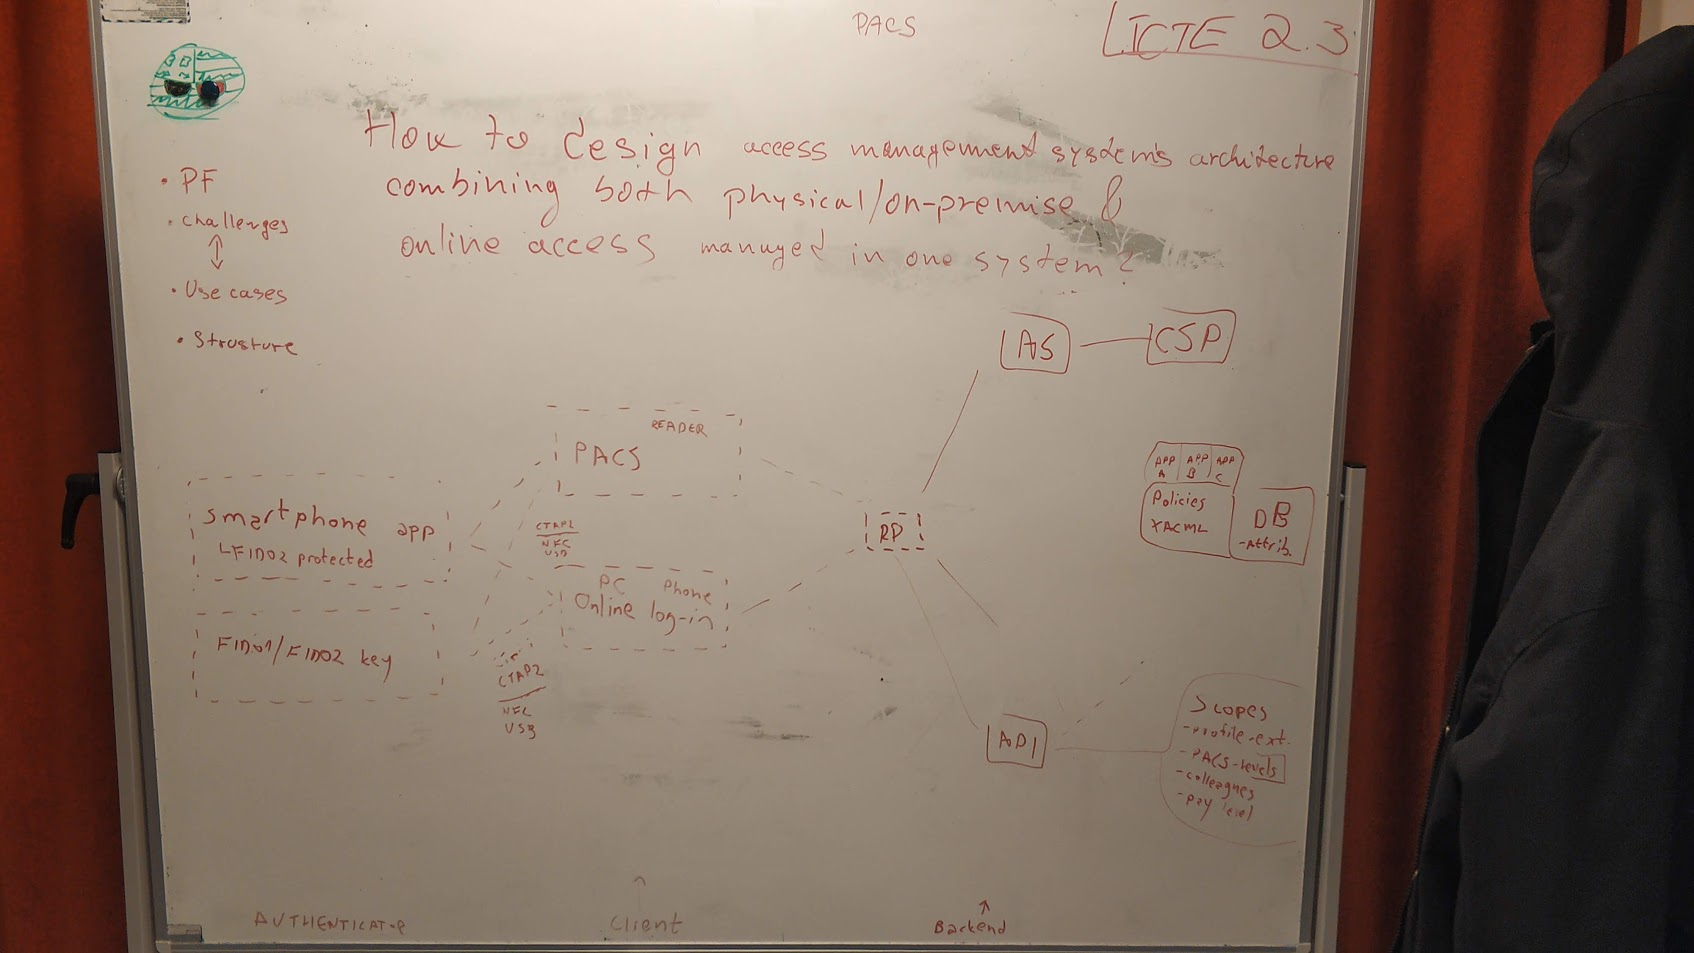
\includegraphics[width=.95\textwidth]{00images/IntroArchitecture}
    \caption{Explanation! + new diagram}
    \label{fig:IntroArchitecture}
\end{figure}

\subsection{Challenges} \label{challenges}

There is a number of challenges, which the current \acrshort{acs} in enterprises are facing. One of the major concerns of every access system is its security. Passwords are often targeted as the weakest link in the system. Every employee has their corporate account linked with many services and is accessing many protected resources. Often employees are forced to change their passwords periodically. Therefore, choosing a weak password and successful phishing attacks are a threat which can be solved by two-factor authentication, but as showed in \acrshort{nist} Special Publication 800-63B \cite{Grassi2017DigitalManagement} there are threats still associated with \acrshort{mfa} such as Social engineering, Phishing attacks or Endpoint compromise. Choosing a right combination of factors for authentication is therefore crucial.

Living in the era of fast technical advance, employees also require convenience when using access systems and carrying around an access card is not the most convenient method anymore, as shown in study by HID~\cite{2017AccessGlobal}, where 61\% of respondents sees integration between systems as hugely beneficial for user convenience or by Netflix~\cite{2012NetflixPilot}, where 87.5\% of respondents would like to use smartphones to open doors in the workplace for authentication. \acrshort{acs} should therefore, offer more convenient ways of authentication -- for example a smartphone.

Often, the physical access control and access policy management systems are two separate entities in enterprises. This requires more resources spend on managing these systems, as well as more set-up work when a new employee is hired or leaves the company. Having one system to handle these tasks is thus desirable.
\subsection{Problem formulation} \label{problemFormulation}
The motivation for this project comes from the existing split of online and physical access control systems. Secondary, the low security of passwords has been demonstrated by several phishing cases and their use is discouraged.
% TODO add reference here
Alternative ways of strong authentication have been proposed instead, including physical cryptographic devices.
% TODO add reference here
The banking industry, which has been using similar tokens for a long period of time already (credit cards), has now witnessed the migration of these tokens to smartphones, mainly for user convenience.
% TODO add reference here
Such migration is also technically possible in access control scenarios, although its use has been limited in practice.

Taking into account the challenges and issues mentioned previously, we propose an innovative \acrshort{acs} that addresses these issues, by building on top of state-of-the-art technologies in the field. The problem formulation is as follows:

\begin{center}
    \textit{“How to design an Access control system, combining both physical and online access control, that includes strong authentication and enables the use of smartphone?”}
\end{center}

\paragraph{Sub-questions}
We define the following sub-problems to help guide us in the analysis and design of the system:

% TODO Is this still draft?
\begin{itemize}[noitemsep]
    \item What solutions are there on the market?
    \item What is the system architecture?
    \item Which technologies are the best for proposed system?
    \item Which components of the system must be implemented for MVP?
    \item What are the requirements of the system?
\end{itemize}
\subsection{Report Structure}


% \pagebreak
% \section{Methodology} \label{Methodology}
TO DO

% Moved it to discussion
% \subsection{Multi-factor considerations} \label{multiFA}

Multi-factor authentication is an approach where two or more factors for successful authentication of a user are required. This way, if one of factors is compromised, there is a need for compromising the other factors as well in order to successfully access the resources. \acrshort{nist} in their Digital Identity Guidelines~\cite{Grassi2017Digital3} specifies three groups of authenticators which can be used for authentication:
\begin{itemize}[noitemsep]
    \item Something you know (typically a password, \acrshort{pin}, etc.)
    \item Something you have (typically a physical cryptographic key, authenticator application, etc.)
    \item Something you are (typically a fingerprint, retina scan, etc.)
\end{itemize}

Choosing a right combination of authenticators is crucial for every system as it can either strengthen the security or if badly combined even weaken it. Therefore, now we will analyse each of these three groups of authenticators and suggest the most suitable one.

\paragraph{Something you know}
Authenticators from this group has been used for centuries, however in the era of technical advance and modern technologies they become obsolete and hard to manage. People are using dozens of services online for which they need to remember some kind of password or \acrshort{pin}. Therefore, they are often choosing easy to remember passwords or are using the same for all services~\cite{} (Online Security Survey REF!). On top of that, passwords are prone to phishing attacks and it is possible a user will forget it. Furthermore, one of the aims of the system presented in this project, is to avoid the use of passwords. Using\textit{ ``something you know’’} as another factor would therefore go against our initial goal of not using this element.

\paragraph{Something you have}
In the enterprise environment, access cards (RFID or proximity cards) are used often, this is just one factor authentication thought. These days, there are many options for authentication using \textit{``something you have’’}, some being more user friendly than the others. It is popular to use a phone to receive a SMS or an email with a \acrfull{otp} to prove identity, but it has been advised by NIST not to use it anymore~\cite{} (REF! NIST Special Publication 800-63-3 | blog). For the purposes of our system, as mentioned before (in section \ref{sec:analysis-authentication}), we are planning to use a physical cryptographic key to authenticate a user as a primary authentication method, instead of \textit{``something you know’’}. Using two physical cryptographic keys is not advised because of a high chance of losing them both at the same time. On the other hand, using \acrshort{otp} generator such as smartphone application or smart card is feasible, because of its simplicity, easy of use and price. 

\paragraph{Something you are}
People tend to forget and lose things; therefore, one can argue that using \textit{``something you are’’} is the most user friendly and secure of all above mentioned authenticators. Fingerprint scan is among the most used authenticators. FIDO2 which is implemented in our system has been certified on Android smartphones and biometric scanners can be used to authenticate users. Another option is to integrate fingerprint scanner to a physical cryptographic key. This way, the ownership of the device and identity of the user can be verified at the same time. Also, it fulfils the NIST requirement about using Biometrics in \acrshort{mfa}: \textit{Biometrics SHALL be used only as part of multi-factor authentication with a physical authenticator (something you have).}~\cite{} (REF! Digital Identity Guidelines: Authentication and Lifecycle Management). Both of these options are suitable for our enterprise scenario and can be proposed to be used.

\paragraph{Suggested solution}
Each of the authenticator types has it pros and cons. The most important criteria for choosing another factor in \acrshort{mfa} are the security and easy of use. Based on analysis above, three candidate solutions are found:
\begin{itemize}[noitemsep]
    \item \acrshort{otp} generator in form of calculator or smartphone application
    \item \acrshort{fido}2 physical cryptographic key with fingerprint scanner
    \item \acrshort{fido}2 certified smartphone with fingerprint scanner
\end{itemize}
All three solution are secure~\cite{}(REF!  Authentication and Lifecycle Management),\cite{} (REF! FIDO2 Project), fairly easy to use and can be implemented to our system. Our preference are both options containing FIDO2 as it is being implemented in the system already. However, as \acrshort{mfa} is not part of the requirements neither for \acrshort{mvp} nor for prototype, we will not go further in analyzing which of candidate solutions is the most feasible to implement.
% \pagebreak
% \section{State of the Art} \label{sec:sota}
TO DO - INTRO
% TODO section intro


\subsection{Basic terms}\label{sec:basic-terms}

\paragraph{Policy}
The IT portfolio of many current enterprises consists of a variety of different applications and systems. As a fine grained control of users' access to these resources is required, management of access rights for every user can become tedious. A set of rules is usually in place, which specify how a \textit{subject} (a person, user, actor) can interact with an \textit{object} (system, program), describing subject's accountability and capabilities within the object~\cite{Feltus2008PreliminaryConcept}. Policies are often used in the \hyperref[sec:xacml]{XACML} context.

\paragraph{Assertion}
An assertion is a ``confident and forceful statement of fact or belief''\footnotemark. In the context of authentication and in particular \hyperref[sec:saml]{SAML}, it is often the case that the identity provider is an independent entity, logically and physically separated from the application/relying party that requested user authentication. After the identity provider authenticates the user, it issues an assertion, confirming that the user's identity has been verified.

\footnotetext{\url{https://en.oxforddictionaries.com/definition/assertion}, accessed 05 March 2019}

\paragraph{Single Sign-on}
Single sign-on systems are such systems where the user only needs to authenticate once to be logged in to different services from different providers~\cite{Suoranta2014LogoutSolutions}. In practice, big common providers, such as Google or Facebook are used to sign the user in, and the user's profile with the provider is then used to access the content or services hosted by a third party.

\paragraph{Multi-factor authentication}
Multi-factor authentication is an approach where two or more factors for successful authentication of a user are required. This way, if one of factors is compromised, there is a need for compromising the other factors as well in order to successfully access the resources. \acrshort{nist} in their Digital Identity Guidelines~\cite{Grassi2017Digital3} specifies three groups of authenticators which can be used for authentication:
\begin{itemize}[noitemsep]
    \item Something you know (typically a password, \acrshort{pin}, etc.)
    \item Something you have (typically a physical cryptographic key, authenticator application, etc.)
    \item Something you are (typically a fingerprint, retina scan, etc.)
\end{itemize}
\subsection{Authentication} \label{authentication_sota}
Authentication is the process of confirming and verifying someone's identity. In this section, we consider \acrlong{oidc} and FIDO as the two main technologies that can be used for online authentication. Afterwards, the NIST framework is presented, as it defines a useful classification model for authentication procedures, based on their security level.

\subsubsection{OpenID Connect}

%REFERENCE NAME TO OPENID STANDARD "Final: OpenID Connect Core 1.0 incorporating errata set 1"
\acrfull{oidc} is an authentication layer standard developed by OpenID Foundation. Current version is OpenID Connect 1.0, which has been proposed in November 2014~\cite{Sakimura2014Final:1}. \acrshort{oidc} is an extension and builds on top of the OAuth 2.0’s authorisation process, which is an authorisation standard and has been described in Section \ref{sec:OAuth_2}. 

As already mentioned, OAuth 2.0 is designated for authorisation but at the time it has been ‘misused’ for authentication purposes by tweaking it and developing different extensions~\cite{RicherUser2.0}. Therefore, there was a need for simple authentication standard which would build on top of the OAuth and that is \acrshort{oidc}.

The purpose of the \acrshort{oidc} is to allow the Client to authenticate (verify the identity) of the user, using the Authorisation server, which also provides identity information of the user, while OAuth 2.0 is being used to obtain access tokens and use them to access resources which are protected~\cite{OpenIDSpecs}. Technically speaking \textit{“OpenID Connect specifies a RESTful HTTP API, using JSON as a data format”}~\cite{OpenIDSpecs}.

Lets take an example of an user accessing a web service which requires log-in (also called \acrfull{rp}). The user needs to log-in first, e.g. using \acrfull{ms} account. User is redirected to the \acrfull{op}, where he has to enter his credentials and afterwards is requested to grand a permission for the service to access specific data from the \acrshort{ms} account, this happens on the Authorisation server
%(\acrshort{op} and Authorization server is the same entitity)
. If the authentication of the user is successful, \acrshort{op} provides \acrfull{rp} with \textit{id\_token} which verifies user’s identity and bears basic user’s information (e-mail, name, birthday, etc.). This \textit{id\_token} is in form of \acrfull{jwt} which defines a way of conveying data as \acrshort{json} object between parties securely, compactly and self-contained. Other token which is obtained during the process is \textit{Access Token}. User is then redirected to post login \acrshort{url}. If the  \acrshort{rp} needs to access protected resources, it uses the obtained \textit{Access Token} and the process continues using OAuth flow explained in Section \ref{sec:OAuth_2}.
\subsubsection{FIDO2}

Fast Identity Online Alliance (\acrshort{fido} Alliance) is an organization developing authentication standards. Protocols like \acrfull{u2f}, \acrfull{uaf} or \acrshort{fido}2 are products of \acrshort{fido} Alliance and its partners. The main aim of \acrshort{fido} is to create phishing-proof, password-less and secure standards. \acrshort{u2f} and \acrshort{uaf} has been proposed in 2014(REF), both being updated and having new versions over time however, the focus will be put towards the newest \acrshort{fido}2 project and its specification rather than older standards.

% TODO add figure reference
The \acrshort{fido}2 project’s aim is to provide phishing-proof, password-less, secure and simple authentication protocol. Fundamental components of \acrshort{fido}2 are WebAuthn which is the \acrshort{api} for a client (by \acrshort{w3c}) and \acrshort{ctap} (by \acrshort{fido}), the \acrshort{api} for the authenticator. These define an abstraction layer which allows strongly authenticated credentials. Therefore, any supported client, being it a native application or browser, running on client’s device and any supported authenticator, being it a build in or roaming authenticator connected to the device via \acrshort{nfc}, \acrshort{ble} or \acrshort{usb}, can use a standardized method to authenticate the user. There are several entities involved in the process of registering and subsequently authenticating the user as it can be seen in Figure XY.

% TODO add reference
\begin{figure}[ht]
    \centering
    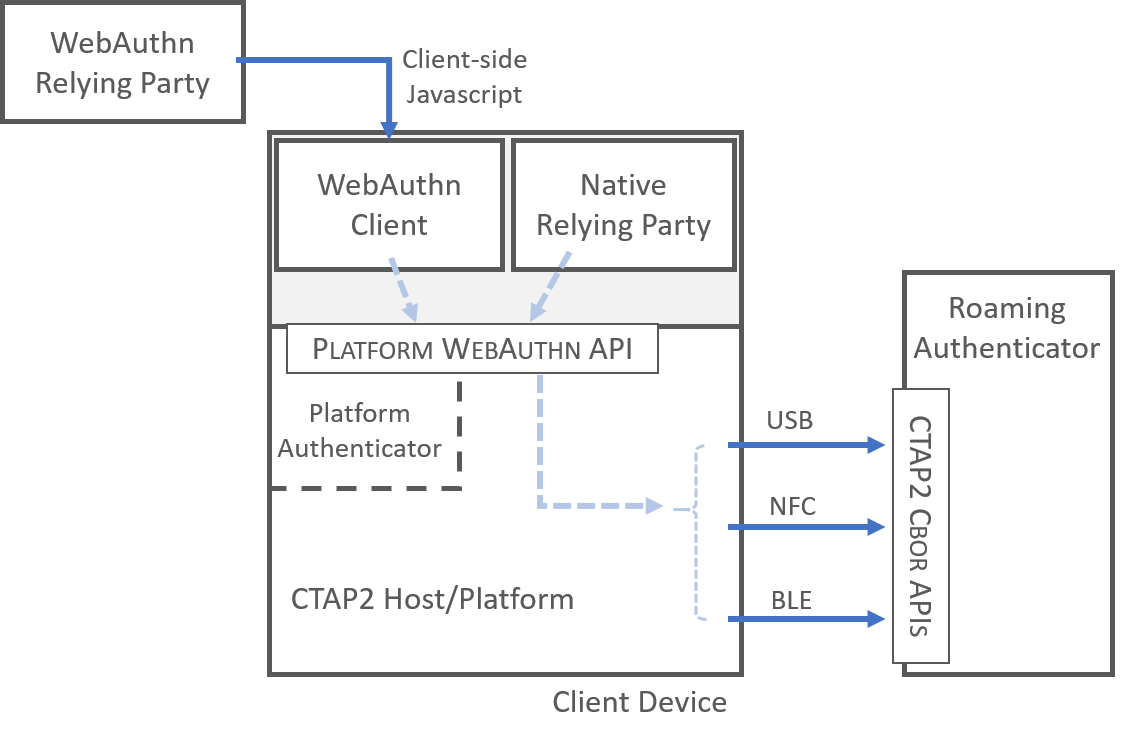
\includegraphics[width=.95\textwidth]{00images/FIDO2_Overview.png}
    \caption{Explanation. From~\cite{}SOURCE}
    \label{fig:fido2_overview}
\end{figure}

\paragraph{Client Device} 
is a hardware which is hosting the authentication via built in or roaming authenticator and communicates with a relying party. Example of such devices are laptops or smartphones. 

\paragraph{Roaming Authenticator} 
is an authenticator which can be connected to different client devices using \acrshort{ble}, \acrshort{nfc} or \acrshort{usb} interfaces. To communicate with a client device, \acrshort{ctap}1 or \acrshort{ctap}2 can be used.

\paragraph{Platform Authenticator} 
is built in on a client device and can only be used with a given device. Example of such authenticators are fingerprint scanners or facial recognition.

\paragraph{Relaying Party} 
is an application or service which requests authenticated credentials. It can be a native or web application.

\paragraph{\acrshort{ctap}2}
\acrlong{ctap} 2 (\acrshort{ctap}2) is the newest version of the \acrshort{ctap} protocol, which is backward compatible the preceding \acrshort{ctap}1/\acrshort{u2f} protocol by mapping \acrshort{ctap}2 request to \acrshort{ctap}1/\acrshort{u2f} and vice versa for responses, unless the relaying party requests a parameter which is \acrshort{ctap}2 specific. 

The \acrshort{ctap}2 specifies the application layer protocol so that authenticator and client device can communicate, as well as it defines how transport layer connection with different physical authenticators should be set up in accordance with the application layer protocol. This enables external devices to be used as authenticators and work with WebAuthn with applications and services.

% TODO add reference
The biggest improvements of \acrshort{ctap}2 over \acrshort{ctap} is the option to verify the user using biometrics or PIN. On top of that, besides storing a private key, devices are capable of storage of associated metadata which allows login even without typing an username. Android phones with android 7.0 and higher can be used as authenticators with their fingerprint or biometric scanners, thanks to a support of Trusted Platform Modules.(REF)

\paragraph{WebAuth} 
Web Authentication (WebAuthn) is the new web standard published on 4th March 2019  by \acrshort{w3c} which defines web \acrshort{api} which enables web browsers and platforms to enable external authenticators using \acrshort{fido} authentication. It standardizes the public-key authentication between users and web applications or services, so it is being used for communication between the client device and a RP.

When a user wants to use authentication with \acrshort{fido}2, given application or website must support it in the first place. User can create a new account or use an already existing one and associate it with the \acrshort{fido}2 authenticator. The authenticator, whether it is a roaming or built-in one, creates cryptographic key pair (private and public key) on user request which has to be confirmed by a user gesture, e.g. fingerprint, biometrics, PIN, touch. Key pair is then created, and the private key is securely stored on the authenticator while the public one, along with associated account details is sent to a server for storage.

% TODO change figure reference
In figure XYZ below, the high level sequence diagram of \acrshort{fido}2 authentication is shown. When a user wants to log-in to a service the relying party sends Credential ID and a challenge to a client, which then forwards this data to authenticator along with Relying party ID and Token binding. In order to proceed with authentication, user's gesture is required. Relying party ID counters the man-in-the-middle attack, making sure that it is always the same party the authentication is done with. Having Credential ID allows to have multiple accounts associated with the same key for the same service and have different key pair for each of the accounts. Authenticator then looks up the private key based on the Credential ID and Relying party ID, which is then used to sign the payload. The signed payload and a signature counter are sent then as an assertion to the client, which forwards it to the relying party together with the initial request. The relying party then verifies the signature with the public key of given account and logs in the user. The signature counter secures the authentication from authenticator clones. In case that the authenticator is cloned and an identical authenticator is produced by a malicious party, incrementing the counter at each sign-in ensures that the state of the original authenticator and its clone divert at some point. Therefore, if the clones is used at some point, it has lower counter than the is supposed to and gets detected and user gets notified.

% TODO add figure source
\begin{figure}[ht]
    \centering
    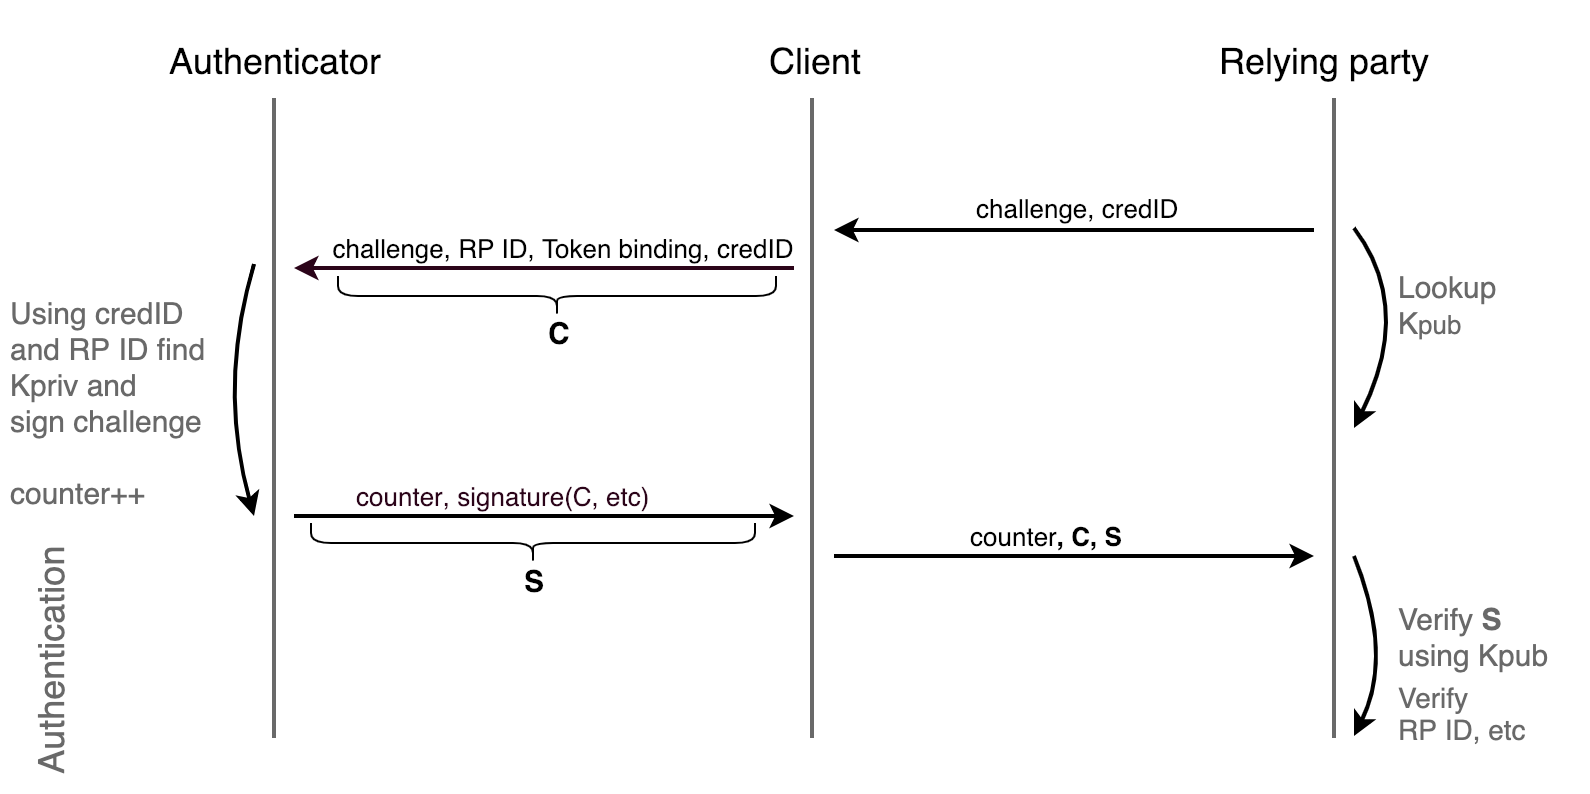
\includegraphics[width=.95\textwidth]{00images/FIDO2_Authentication.png}
    \caption{Explanation. From~\cite{}SOURCE}
    \label{fig:fido2_authentication}
\end{figure}
\subsubsection{NIST Digital Identity Guidelines}

The \acrfull{nist} developed a set of guidelines, intended primarily to govern how public authorities in the US implement digital authentication in non-national-security scenarios. However, it was adopted by a wider community, spanning out of the government sector~\cite{Grassi2017GovernmentCollaboration}.

The guidelines contain three volumes, covering three distinct areas of authentication:
\begin{enumerate*}[label=(\roman*)]
    \item SP 800-63A focused on Enrolment and Identity Proofing;
    \item SP 800-63B centred around Authentication and Lifecycle Management; and
    \item SP 800-63C covering Federation and Assertions.
\end{enumerate*}
The guidelines advertise the use of authentication to mitigate risks of unauthorised access to protected resources, but also promote minimising the collection of \acrfull{pii} and use of pseudonymous information whenever possible~\cite{Grassi2017Digital3}.

The guidelines define a Digital Identity Model (Figure~\ref{fig:nist-model}), which is useful to distinguish the various types of roles and activities within an authentication system. On the left side of the model there is a \acrfull{csp}. \acrshort{csp} is an entity that issues electronic credentials and registers user's \textit{authenticator} (authenticator is something that the user has or controls). On the right side of the model is the verifier, whose task is to authenticate users by validating binding of their authenticators to their credentials~\cite{Grassi2017Digital3}.

 \begin{figure}[ht]
    \centering
    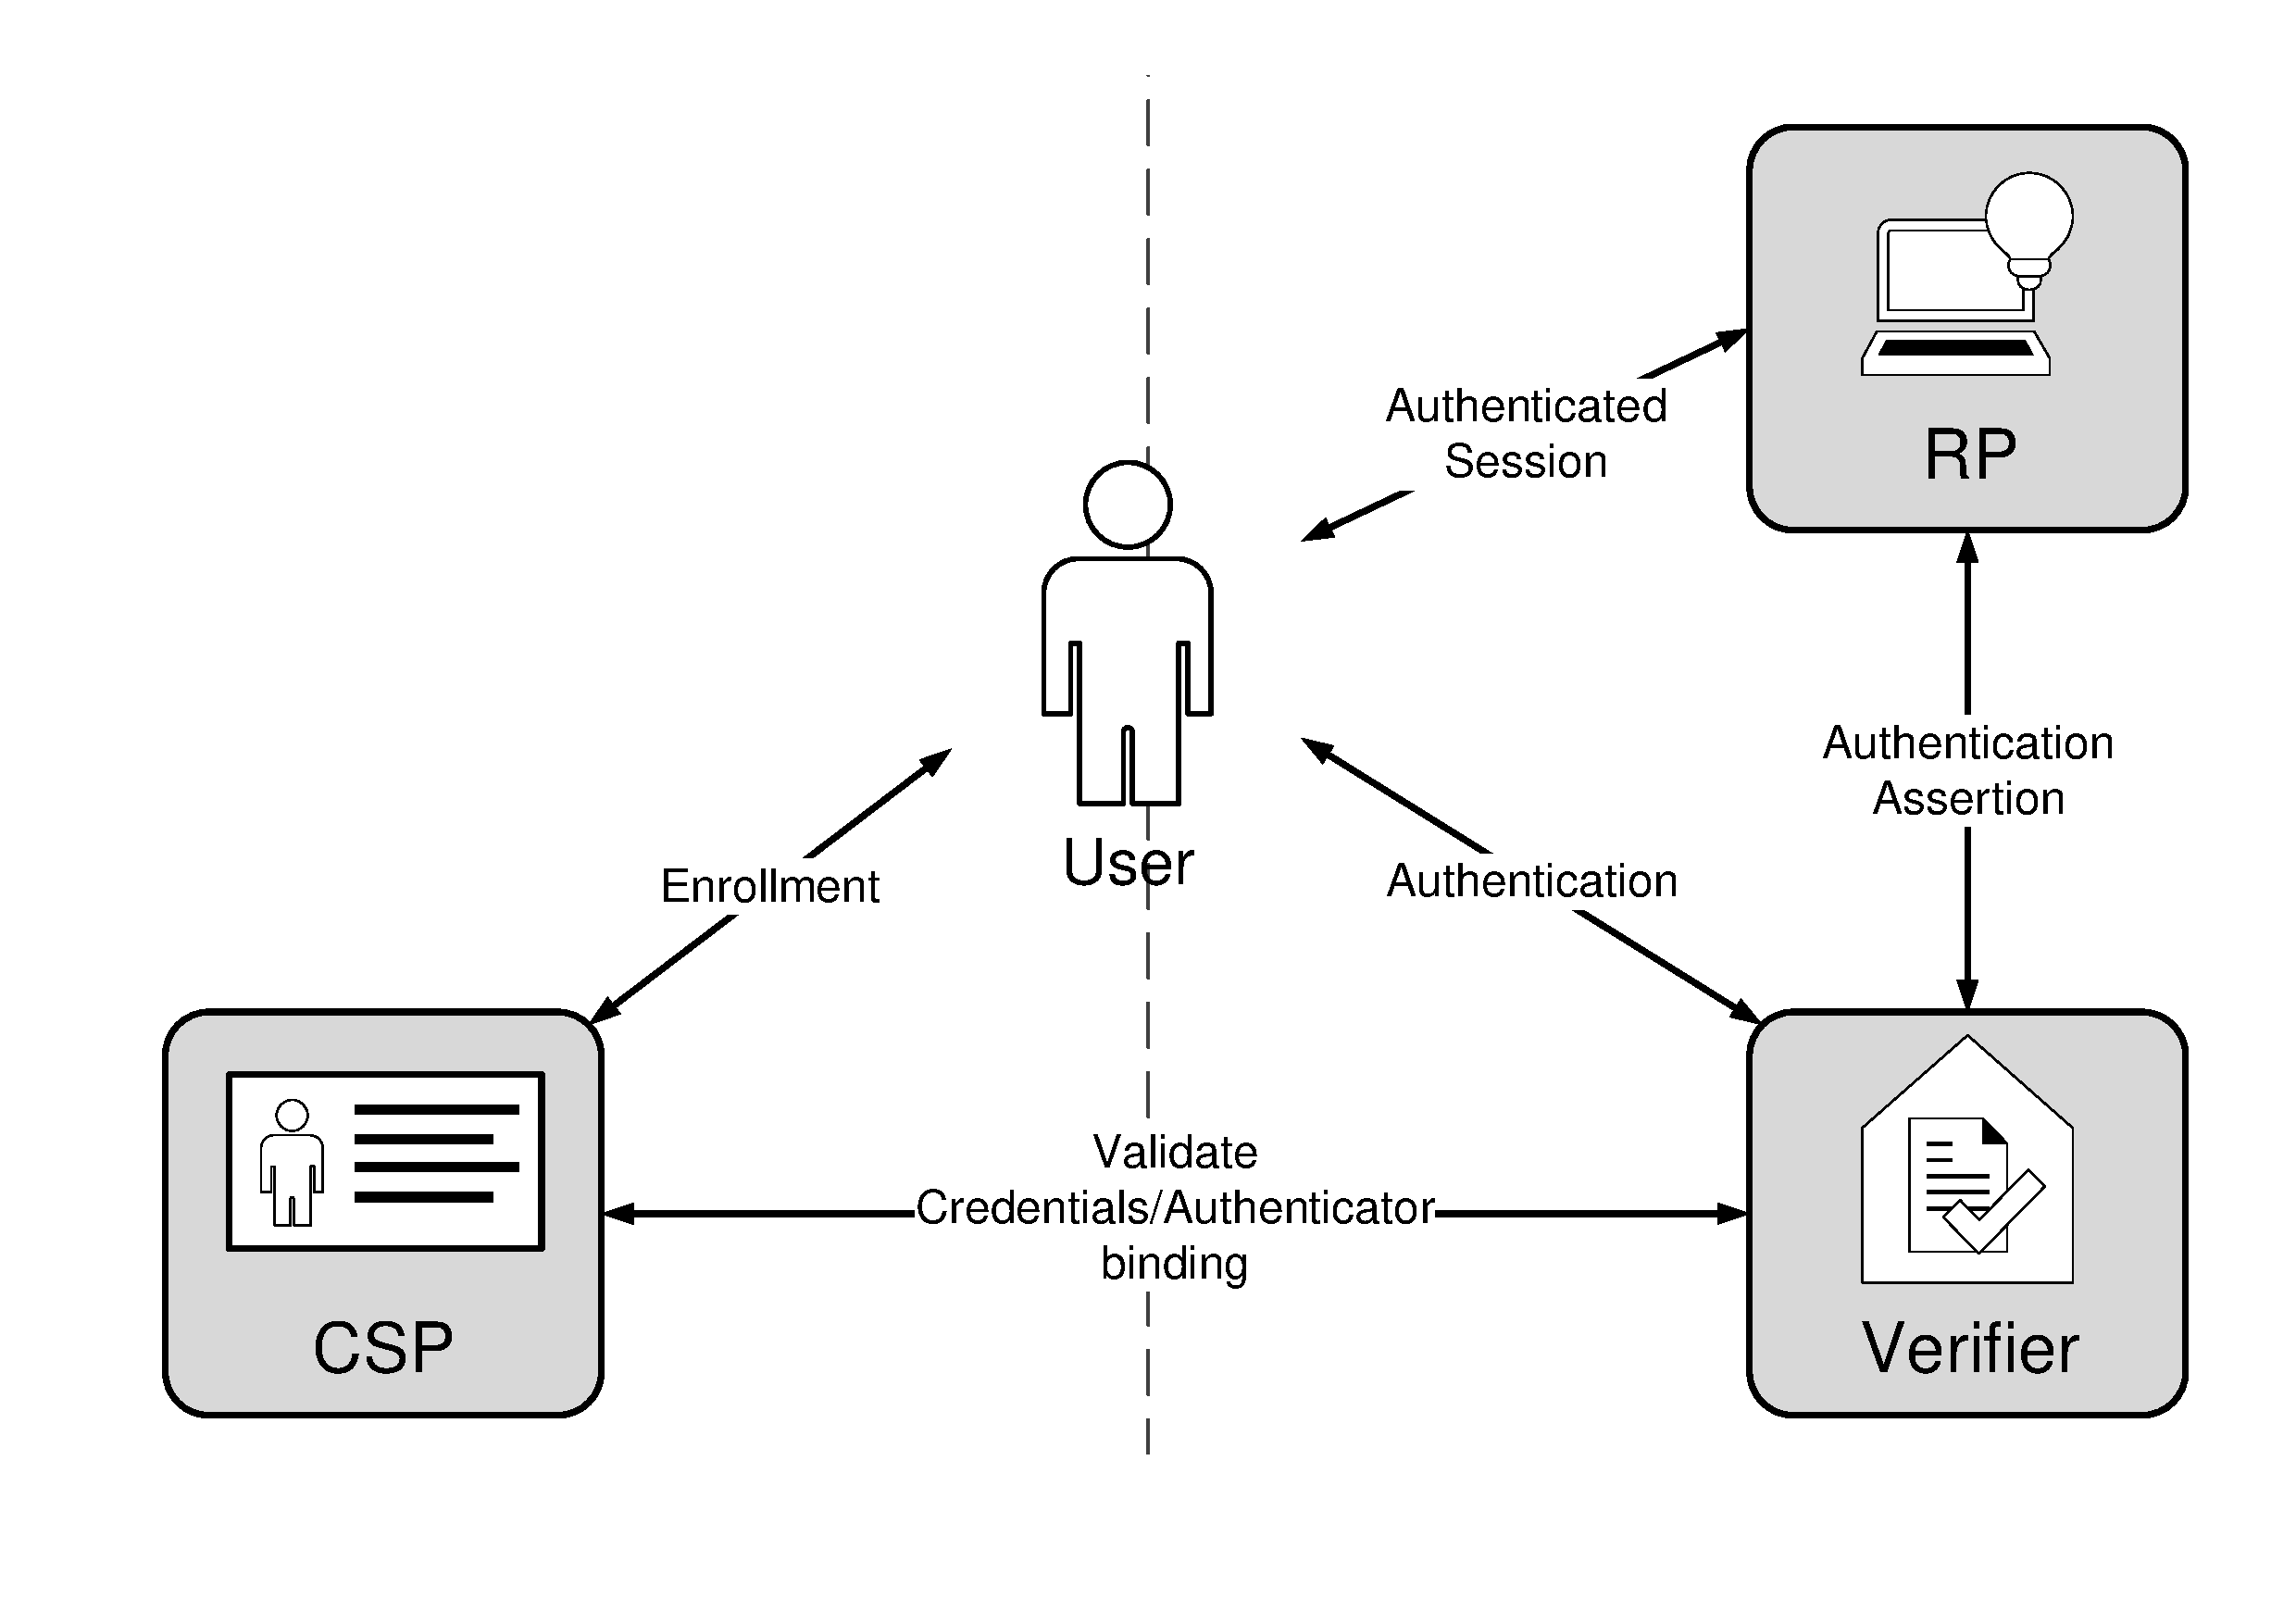
\includegraphics[width=.95\textwidth]{nist-simplified}
    \caption{Digital Identity Model (simplified). The left side of the figure represents enrolment of the user with the \acrshort{csp}. The right part of the user represents authentication with the verifier, before an authenticated session is established between the user and the \acrshort{rp}. Taken from~\cite{Grassi2017Digital3} (edited).}
    \label{fig:nist-model}
\end{figure}

\paragraph{SP 800-63A}
This volume of the Digital Identity Guidelines defines three Identity Assurance Levels (IALs) and requirements on identity proofing for each level. The \acrshort{ial}1 requires no verification of assertions provided by the user. \acrshort{ial}2 requires either remote or physically-present verification of assertions made by the user, while \acrshort{ial}3 requires manual verification by a trained person, representing the \acrshort{csp}~\cite{Grassi2017DigitalProofing}.

\paragraph{SP 800-63B}
The B volume of the Guidelines defines three Authenticator Assurance Levels (AALs).

To authenticate themselves in AAL1, the user needs to demonstrate control of one authenticator. This must be done through a secure authentication protocol.

In AAL2, the user must demonstrate control of two distinct authenticators. This can be in a form of a multi-factor authenticator, or single-factor possession-based authenticator together with a memorised password. Cryptographic techniques defined in~\cite{Evans2001SECURITYMODULES} must be used.

In AAL3, a hardware-based authenticator must be used in addition to requirements of AAL2. Furthermore, one of the authenticators used must be resistant to attacks attempting to impersonate the user.

\paragraph{SP 800-63C}
The C volume of the guidelines describes the use of assertions for identity federation across several \acrshort{rp}s~\cite{Grassi2017DigitalAssertions}. This enables the user to use services provided by several \acrshort{rp}s, while maintaining only a single identity at one \acrshort{idp}. The volume also describes three Federation Assurance Levels, however we do not cover these in this report.
\subsection{Authorization} \label{authotization_sota}
TO DO - INTRO

\subsubsection{OAuth 2.0} \label{sec:OAuth_2}

Before existence of OAuth, the access to user's protected resources was commonly delegated to a third party by sharing the user's credentials with that third party. It typically meant, that a client application asked the user for their user-name and password and these were then used to log in to a given service on behalf of the user. This approach was named the `password anti-pattern' and is flawed~\cite{Paul2010OAuthAnti-pattern}. Besides the risk of compromising user's account if the credentials leak from the client application, it is also not possible for the user to fine-tune the access to their account and set up different levels of access for different client applications. 

The OAuth 1.0 was published in 2010 as to address this problem~\cite{Hammer-Lahav2010TheProtocol} and was followed in 2012 by OAuth 2.0~\cite{Hardt2012TheFramework}. OAuth 2.0 is not compatible with version 1.0 and is widely used today. For the rest of this report we will refer to OAuth 2.0.

Using the OAuth framework, a third-party application may obtain a fine-grained access to protected resources. The third-party application requesting access to user's protected resources is known as the \textit{client}. The server controlling the access to the protected resources is known as the \textit{authorisation server}. The standard defines four distinct ways (called \textit{grant types}), how the client can obtain the access by communicating with the authorisation server. Before we describe these grant types, let us first draw the difference between the different clients.

\paragraph{Client types} OAuth distinguishes three client types:
\begin{itemize}[noitemsep]
    \item \textit{Web-based application} is an application that runs on a web server and communicates with the user over HTML via a browser. Web-based application is considered secure, as the client secrets can be stored on the web server.
    \item \textit{User-agent-based application} is downloaded from the server, but afterwards runs on the user's device. This is considered less secure than web-based application, as any secrets could be potentially exposed by the user-agent (browser).
    \item \textit{Native application} is installed by the user and runs directly on user's device. It can offer good protection to secrets entered by the user during runtime, but any application secrets which are included and shipped with the application could be potentially exposed~\cite{Hardt2012TheFramework}.
\end{itemize}

\paragraph{Grant types} Four grant types are defined by the standard. Not all grant types are suitable for all client types, but other parameters, such as desired level of security or preference also influence the choice of the grant type. The defined types are as follows:

\begin{itemize}[noitemsep]
    \item \textit{Authorisation Code Grant}. Using this grant type, the user is first directed from the web-based application to authenticate with the authorisation server. After user authenticates, they are asked by the authorisation server to give consent for the client application to use their protected resources. Once the consent is given, the user agent receives an authorisation code from the authentication server. This authorisation code is passed to the web server via a \acrshort{http} redirect method. The client running on the web server contacts the authorisation server with the authorisation code to obtain an access token. The access token is presented when the client application accesses the protected resource. This flow is illustrated in Figure~\ref{fig:oauth-code-grant}.
    \item \textit{Implicit Grant}. In this grant type, the client application is typically running in the user agent. The flow is similar to the one described above, but instead of the authorisation code, the access token is sent directly to the client application. This is simpler than the authorisation code grant, but less secure, since the access token can be captured by other applications residing on the user's device.
    \item \textit{Resource Owner Password Credentials Grant}. When using this grant type, user's credentials need to be shared directly with the client application. This is only suitable, if the client application is fully trusted by the user.
    \item \textit{Client Credentials Grant}. Is used when the client application requires access to own resources (as opposed to user's protected resources).
\end{itemize}

\begin{figure}[ht]
    \centering
    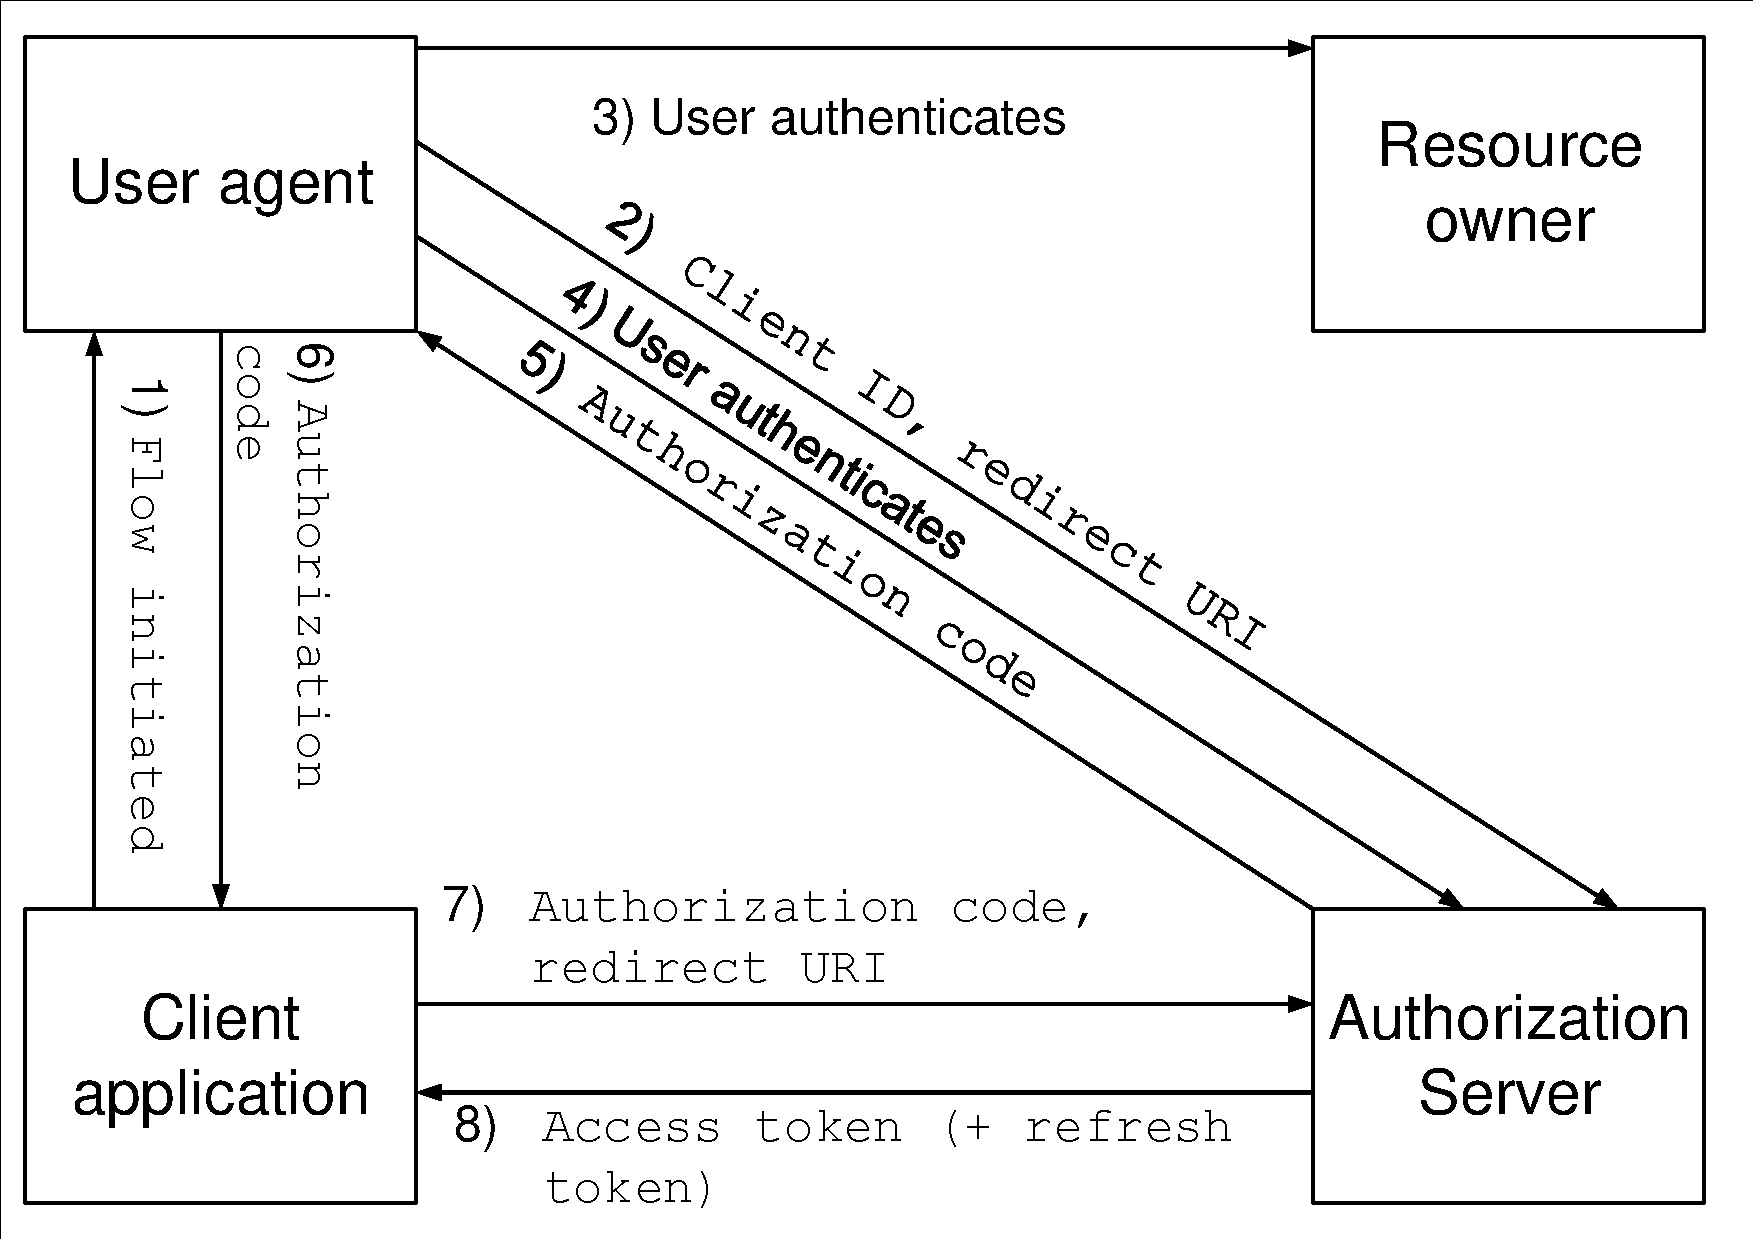
\includegraphics[width=.95\textwidth]{oauth-code-grant}
    \caption{OAuth Authorisation code grant. The user authenticates with the authorisation server and gives consent for access to their protected resources. An authorisation code is sent to the redirect URI specified in the original request. This access token is forwarded to the web server hosting the client application and exchanged for an access token at the authorisation server. From~\cite{Hardt2012TheFramework}, edited.}
    \label{fig:oauth-code-grant}
\end{figure}

\paragraph{Access token scopes}
Scope in the OAuth context typically represents a piece of functionality or data, access to which can be individually controlled. Well defined scopes allow for granular access control. The client application includes the \textit{scope} parameter in the authorisation request to inform the authorisation server, which data or functionality it wishes to access. The authorisation server may grant access to any number of the requested scopes, based on the internal policy and user's consent~\cite{Hardt2012TheFramework}.

The process outlined above is mostly concerned with authorisation of the client to access protected resources. However, it emerged as a common, albeit incorrect practice that OAuth was used to authenticate users~\cite{RicherUser2.0}, by allowing the client to only read a scope that contains the basic user data. While it is technically possible to achieve this using OAuth alone, \acrshort{oidc} was developed to standardise this usecase. We cover \acrshort{oidc} these in Section~\ref{sec:oidc}.
\subsubsection{SAML}\label{sec:saml}

The \acrfull{saml} is a framework for exchange of assertions containing security information between two online parties, typically an identity provider and a relying party. Similarly as XACML, \acrshort{saml} was developed by OASIS. Version 1.0 was released in 2002 and version 2.0 (latest) in 2005. The rest of this report refers to version 2.0.

The main premise of \acrshort{saml} is that the \acrfull{idp} and the protected resource/application are two separated entities. This is desired, since it enables us to manage identities centrally for multiple applications and avoids duplication of user accounts across these applications. Moreover, separating these enables both parts to specialise only in their task.

The Figure~\ref{fig:saml-architectire} illustrates the separation of these two entities. It also depicts the high-level flow of the authentication process. If the user wants to access the protected resource on the right, they first need to authenticate themselves with the \acrshort{idp}.

Another noteworthy aspect of \acrshort{saml} is the identity federation. This is achieved, when the \acrshort{idp} and the \acrshort{rp} are in different security realms, possibly operated by different organisations. As long as an agreement is established between the two, users can use their online identity, managed by the \acrshort{idp}, to access any resources outside the organisation's boundary~\cite{2008SecurityOverview}.

 \begin{figure}[ht]
    \centering
    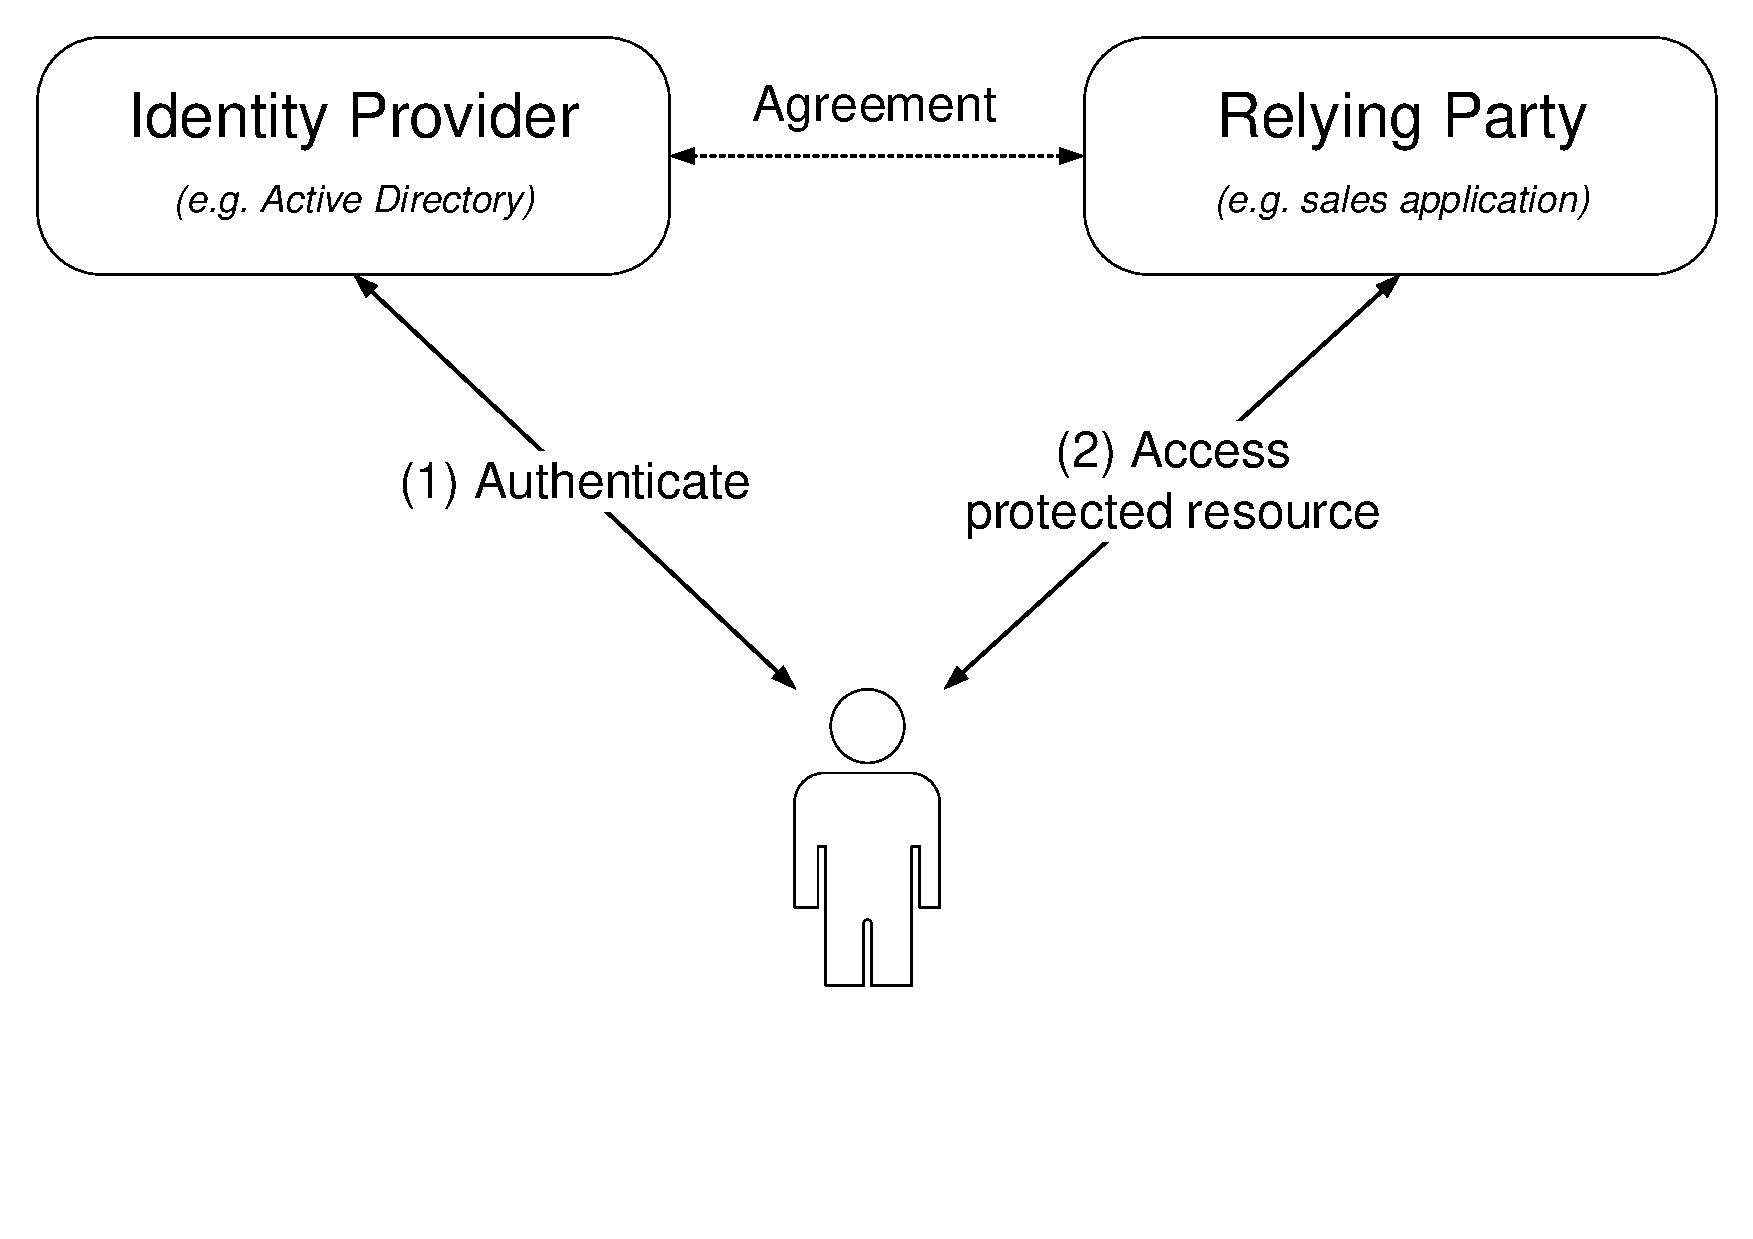
\includegraphics[width=.75\textwidth]{saml-architecture}
    \caption{The general use case of SAML, demonstrating the premise of functional separation of \acrshort{idp} and \acrshort{rp}. Taken from~\cite{2008SecurityOverview}.}
    \label{fig:saml-architectire}
\end{figure}

\paragraph{Assertions}
An assertion in \acrshort{saml} contains some security information about the \textit{subject}. Subject could be the user Bob and the associated information could be Bob's email address and job title. The security information need to be of one of following three categories:

\begin{enumerate*}[label=(\roman*)]
    \item \textit{Authentication statements} describe the means and the timestamp of the authentication carried out by the asserting party;
    \item \textit{Attribute statements} provide information about the subject; and
    \item \textit{Authorisation decision statements} describes what the subject is permitted to access in the system.
\end{enumerate*}

While \acrshort{saml} is widely adopted in the industry and is considered generally secure, numerous security flaws have been identified over time. Most of these arose from improper implementation of the protocol and have been patched since discovery~\cite{Krawczyk2014SecureAttacks}. The vulnerabilities included XML signature wrapping, assertion eavesdropping~\cite{Chen2014Environment-BoundAssertions} and XML parsing issues~\cite{Degges2018AVulnerability}.
\subsection{Access Policy Management} \label{APM_sota}
Choosing a right model for Access policy management is crucial, if a model not suitable for the organisation's needs is chosen it can cause complications in managing employees and resources. We look into Role based and Attribute based access control and their main principals. Then \acrshort{xacml} is looked into as the Attribute based access control standard.
\subsubsection{Role Based Access Control} \label{RBAC_SOTA}

\acrfull{rbac}\footnote{\url{https://csrc.nist.gov/projects/role-based-access-control, accessed 01 April 2019}} is a method of controlling access of users in the system, being it physical or online access in the enterprise. It uses policy neutral approach based on roles, where every employee has a role/s assigned, which defines the access levels and resources to be accessed. Mandatory Access Control (MAC) and Discretionary Access Control (DAC) can also be implemented within the system, even though it is different from them. \acrshort{rbac} creates a structure, where firstly the list of privileges (actions, resources, access levels) is defined and assigned to roles. Each role contains a set of privileges and is part of a group where more roles are gathered. Each employee is then assigned a group/s or directly a role/s which authorizes him to access certain resources. This allows more effective management of employees.

The biggest drawback of \acrshort{rbac} is the process of assigning roles and groups being manual, based on request, and not automated. Therefore, when an employee changes a position in a company and new roles is assigned, the previous one should be revoked, but that is often not done and the employee of is granted the access to resources further. Also, it can take a long time before a new role is assigned. On top of that, in case that an employee leaves a company and his access is not revoked, he may still be able to access resources, which is a security threat to a company. Audit of roles and employees’ assignment to them is needed.

\begin{figure}[ht]
    \centering
    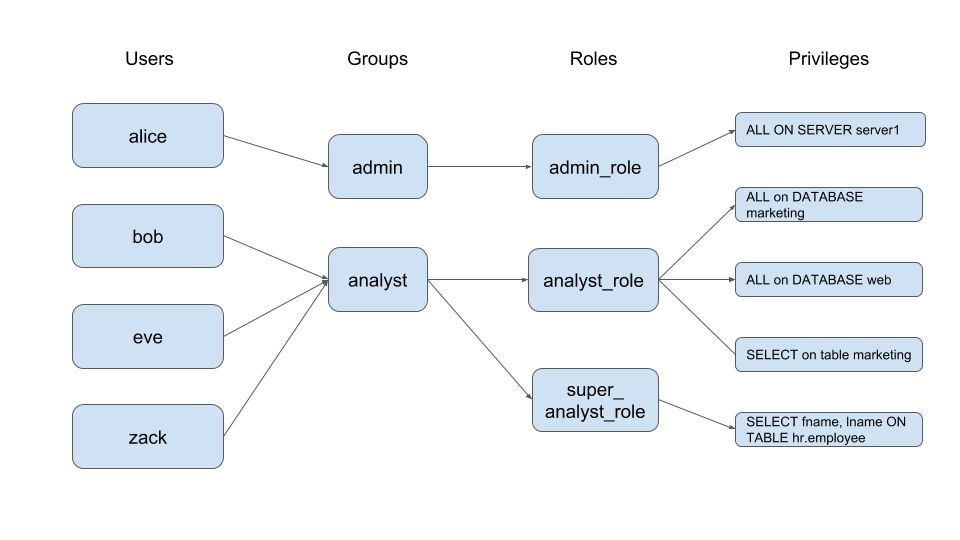
\includegraphics[width=.95\textwidth]{RBAC}
    \caption{Explanation! + new diagram}
    \label{fig:RBAC_diagram_sota}
\end{figure}
\subsubsection{Attribute Based Access Control} \label{sec:sota-abac}

\acrfull{abac} is an automated access control model by NIST\footnote{\url{https://csrc.nist.gov/projects/abac/}, accessed 01 April 2019}. In its core it is based on automatic execution of granting and denying the access depending on attributes and policies. \acrshort{rbac} can be also referred to as Policy (\acrshort{pbac}) or Claims (\acrshort{cbac}) Based Access Control\footnote{\url{https://www.hpl.hp.com/techreports/2009/HPL-2009-30.pdf}, accessed 01 April 2019}. XACML standard is based on \acrshort{abac} and is explained in Section \ref{sec:xacml}. It is often denoted as the evolution of \acrshort{rbac}. This model can implement \acrshort{mac} and \acrshort{dac} models as well.

In \acrshort{abac}, access is assigned based on attributes and characteristics of the user – subject which is making the request, environment conditions and information asset – resource object that is requested. With the help of these attributes, granular policies for granting and denying access can then be established. Every policy combines a set of attributes and is executed by the Boolean logic, e.g. IF the requester is an accountant, THEN allow read access to contracts.

% TODO explanation
\begin{figure}[ht]
    \centering
    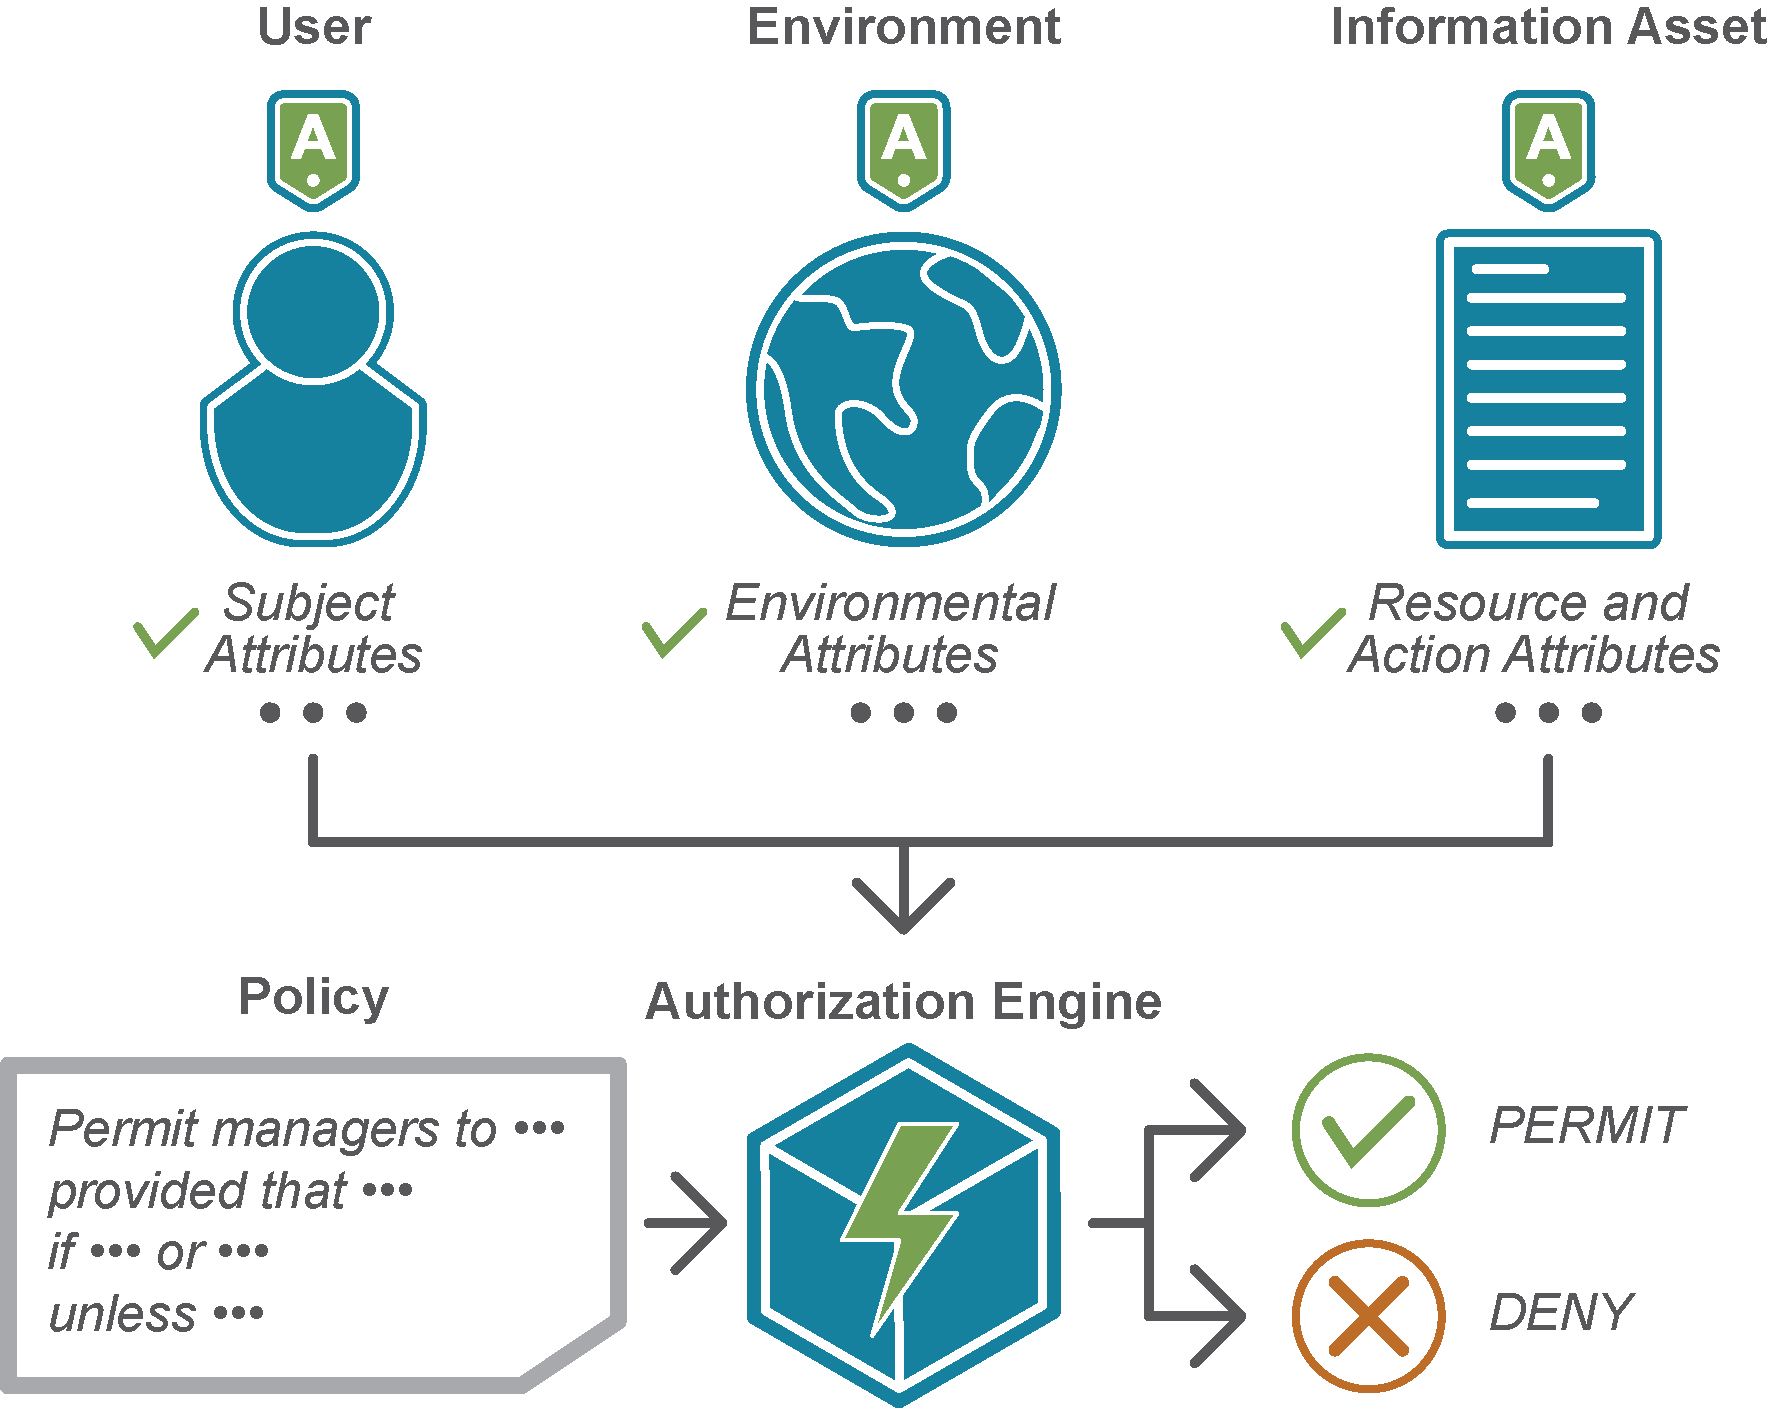
\includegraphics[width=.7\textwidth]{ABAC}
    \caption{Explanation XYZ! + Taken from~\cite{AttributeABAC}.}
    \label{fig:ABAC_diagram_sota}
\end{figure}
\subsubsection{XACML}\label{sec:xacml}

 \acrfull{xacml} is a standardised, XML-based language for expressing security policies. It provides methods to define and combine policy sets and to rapidly identify, which policy applies to a given subject. \acrshort{xacml} was first standardised by OASIS\footnote{\url{https://www.oasis-open.org/}, accessed 04 March 2019} in 2003 and the latest version is XACML 3.0, from 2013~\cite{OASISStandard2013EXtensible3.0}. The further description is based on this latest version.
 
\acrshort{xacml} defines, how the \acrfull{pdp} which evaluates an input (access requests) against a policy set and issues an output -- a decision (such as \textit{access granted}). \acrshort{pdp} resides in an ecosystem comprised of other components that are necessary to maintain and enforce the access policy decisions (see Figure~\ref{fig:xacml-architecture} in Appendix~\ref{sec:analysis-access-policy} on page~\pageref{fig:xacml-architecture}). The other components in this ecosystem are out of scope of the \acrshort{xacml} specification~\cite{OASISStandard2013EXtensible3.0}.

\acrshort{xacml} defines the formal language of the policy set and of the requests/responses. A policy set contains one or more \textit{policies} and a \textit{policy combining algorithm}. The main components of a policy are:
% 
\begin{enumerate*}[label=(\roman*)]
    \item a \textit{target} to which this policy applies and
    \item one or more \textit{rules}.
\end{enumerate*} 
% 
The rule must specify a \textit{target} to which it applies and an \textit{evaluation} (\textit{permit} or \textit{deny}). It can also optionally specify \textit{conditions}, \textit{obligations} and \textit{advices}, all of which further shape the scope of the rule. Policy combining algorithm specifies the order and other conditions that decide, which policy will be finally applied on the request~\cite{OASISStandard2013EXtensible3.0}.
 
The \acrshort{xacml} standard defines in detail several logical entities and their interactions. The native format for messages between these entities is XML, but a profile has been developed to support JSON message format~\cite{2017JSON1.0}. Additional profile was also created to describe implementation in a RESTful architecture~\cite{2017REST1.0}.
 
 Several implementations of \acrshort{xacml} exist in Java, Python and other languages. Criticisms of \acrshort{xacml} include low adoption rate, unsuitability for federated enterprises~\cite{Cser2013XACMLDead}, and lack of transparency for the end user~\cite{Cser2013XACMLDead, Ardagna2011ExpressiveApplications}.


\subsection{Existing access control systems} \label{competitors_sota}

In this section we describe the major players on the market of access control solutions. First we focus on online access control, including device log-in, \acrshort{sso} and directory services. Next, we focus on physical and hybrid access control, comprising access control to protected physical premises and hybrid model that offer physical and online access control. For each category we describe a single vendor, who has significant position on the market and who's offering can be used as a benchmark.

\subsubsection{Online access control -- Microsoft}\label{sec:online-access-control}

For the online access control, we choose Microsoft and its Azure Active Directory (Azure AD)\footnotemark as the benchmark solution, as it is described as ``the leader in its field''~\cite{Kreizman2018MagicWorldwide}. It offers directory services, user authentication and authorisation of users' application access as the core of its functionality, and is primarily targeted on enterprises and organisations, irrespective of size. Microsoft claims that in 2013 50\% of companies on the Fortune~500 list were already using Azure AD and by 2017, this number has grown to 90\%~\cite{Martin201350Azure}.

\footnotetext{\url{https://azure.microsoft.com/en-us/services/active-directory/}, accessed 25 March 2019}

\paragraph{Authentication} Azure AD uses passwords as the primary user authentication method and this setting cannot be changed~\cite{Flores2019AuthenticationMethods}. To provide additional security, \acrlong{mfa} can be enabled. Additional factors that are supported by the solution include:
\begin{enumerate*}[label=(\roman*)]
    % \item \textit{security questions},
    % \item \textit{email address},
    \item \textit{SMS} and \textit{voice call},
    \item \textit{Microsoft Authenticator application},
    \item \textit{one-time passwords}, and 
    \item \textit{OATH hardware tokens}\footnotemark~\cite{Flores2019AuthenticationMethods}.
\end{enumerate*}

Either the enterprise administrator or the user themselves can decide, which of these is used as the second authentication factor. Once enabled, the second factor is always required during user sign-in. Exceptions to this can be defined based on countries, locations, or IP ranges. Moreover, email address and security questions can be added by the user as an additional factor, which can only be used during password recovery, but not during sign-in~\cite{eross-msft2018ConfigureAuthentication}.

\footnotetext{Note, that \acrshort{oath} is different from OAuth. \acrshort{oath} hardware tokens are \acrshort{otp} devices following the reference architecture defined by \acrfull{oath}.

\url{https://openauthentication.org/}, accessed 25 March 2019}

\paragraph{Single Sign-on} Azure AD supports both \acrshort{saml} and OAuth + OpenID Connect for single sign-on to non-Microsoft applications. Developers are encouraged to only use OAuth + OpenID Connect for new applications, but \acrshort{saml} can still be used with legacy and other software that does not support OAuth + OpenID~\cite{barbkess2019SingleDirectory}. 

All four types of authorisation grants (explained in Section \ref{sec:OAuth_2}) defined in OAuth specification can be used. The ID token which is issued during the OpenID connect flow, contains the standard claims defined in the specification. Two endpoints are defined to handle OAuth + OpenID Connect protocols -- v1.0 and v2.0. Together, the two endpoints support variety of languages (.NEt, JavaScript, Python, Java and other) and target applications (on-premise, cloud-based, hybrid)~\cite{deGuzman2018AboutPlatform}.

Azure AD further supports password-based, HTML header-based  and Integrated Windows Authentication \acrlong{sso}~\cite{barbkess2019SingleDirectory}. These are out of scope for this report.

\paragraph{Application access policy management} When a new application is integrated with Azure AD, the access to this application needs to be provisioned to users. This can be done on an individual or a group basis (role-based access control). 

Attribute-based access control is also implemented to a limited degree via use of the \textit{conditional access} method. When this method is in use, additional parameters can be evaluated, such as location, whether \acrshort{mfa} has been used, whether the user is using a compliant device and other predefined attributes. Furthermore, the enterprise administrator can further define custom criteria that need to be met (such as authentication with an external provider)~\cite{Vilcinskas2019WhatAccess}.
\subsubsection{Physical and hybrid access control -- HID Global} \label{sec:pacs-hid}

For the physical and hybrid access control, HID\footnote{\url{https://www.hidglobal.com/}, accessed 02 April 2019} is chosen with its HID Mobile access and Extended Access solutions. HID is one of the leading companies~\cite{TopManufacturers} on the market offering access controls, identity management or \acrshort{iot} solutions. Targeting mostly enterprises with the offer of the whole package, including software and hardware, tailored for the need of an enterprise. Both technologies we cover are designed and implemented based on enterprise’s needs. Because of that, no detailed documentation explaining the working of the system and its technologies is available. The following is a summary of what HID can offer with their system, which may be relevant for our proposed system.

\paragraph{HID Mobile Access}
Mobile Access by HID\footnote{\url{https://www.hidglobal.com/solutions/hid-mobile-access-solutions}, accessed 02 April 2019} is a physical access solution for enterprises, which replaces, or supplements access cards. The solution focuses mostly on the physical access, where mobile devices such as smartphones, wearables or tablets can be used for authentication and granting the access. \acrshort{ble} and \acrshort{nfc} is used~\cite{HIDGlobal2014HIDGlobal} for communication with a mobile-enabled readers. Devices with different operating systems (Android, iOS, BlackBerry) are supported as long as they are \acrshort{nfc} or \acrshort{ble} enabled. When accessing the premises, two modes of communication with a reader are offered: 
%
\begin{enumerate*}[label=(\roman*)]
    \item \textit{Twist\&Go} - where a device can be a few meters from a reader and has to be twisted to begin authentication (utilising \acrshort{ble}),
    \item \textit{Tap\&Go} - where the device has to be swiped over a reader to be authenticated (using \acrshort{nfc}).
\end{enumerate*}
%
HID Secure Identity Service is used for managing employees’ Mobile \acrshort{id}s. Once a Mobile \acrshort{id} is created in the system, the employee receives an invitation with access codes, downloads the application, enrols into it and starts using it without further dues. As the case study at Netflix showed~\cite{2012NetflixPilot}, employees find mobile access intuitive and 90\% of surveyed employees found it easy to use.

\paragraph{Extended Access}
HID offers an Extended Access Technologies\footnote{\url{ https://www.hidglobal.com/extended-access-technologies}, accessed 02 April 2019} besides their physical access. The idea behind is to use the same credentials and an `authenticator' throughout the enterprise during the day, instead of several, which is more convenient for the employee and offers a wider range of applications for the enterprise. It also offers the policy management endpoint from which the accesses are managed. A Trusted Identity~\cite{2018ExperiencingPredictive} is used, which means that an employee’s ‘authenticator’ is verified once and can be used freely afterwards. This Trusted Identity can be built into smartcards, wearables or a smartphone application, allowing the use of printers, payment at the canteen, booking of meeting rooms, accessing premises, etc. All with a single device that has been once verified. In the case of a smartphone application and for physical access to premises, every single employee can be individually identified, even if a crowd is moving through a door. In case of higher security measures, multi-factor authentication can be enabled and biometrics or \acrshort{pin} can be used. On top of that, the system provides advanced predictive analytics for better optimisation of a work place. 
% Unfortunately, no additional information is shared by HID publicly, besides brochures, and therefore, we cannot look into what technologies they are using. The only obvious technologies are \acrshort{ble} and \acrshort{nfc}.
% \pagebreak
% \section{Analysis}\label{sec:analysis}

Building up on our initial idea and problem formulation, we determine two major functional areas that must be supported by our proposed system:

\begin{itemize}[noitemsep]
    \item \textit{\acrfull{pacs}} (access to restricted premises in a company or institution, building access control etc.)
    \item \textit{Online Access Control} (access to computer systems, applications, online sign-in etc.)
\end{itemize}

While the  typical question in a \acrshort{pacs} would be ``\textit{Is the person allowed to enter beyond this point}?'', and can be controlled by a variety of physical barriers, doors, turn-sites and the like, the online access control is more complex. Enterprises nowadays operate a wide spectrum of software solutions including on-premise applications, legacy systems, cloud-based and \acrshort{saas} applications, internally or externally oriented \acrshort{api}s and databases. All of these require some level of access control. To break down this structure, we first begin by identifying two service classes:
\begin{enumerate*}[label=(\roman*)]
    \item \textit{internal applications}, that sit within the enterprise security realm; and 
    \item \textit{external applications}, that include cloud based software, \acrshort{saas} solutions and partner/vendor applications, and which reside outside the given security realm.
\end{enumerate*}

The external applications can be further divided based on their interactions with the internal systems. Applications that are not business critical and/or are not integrated with the business processes may not require access to protected resources at all. Examples of such applications would be a lunch booking system or a company social network. These would be primarily used by the employees, but would not require connectors to business-critical systems and could therefore reside outside the security realm.

Other external applications, however, may require access to business-critical resources for their functions. \acrlong{crm} or payroll system may both be purchased as a \acrshort{saas}, but both require connectors to the protected resources to properly fulfil their functions. We can therefore extend our classification of the external applications accordingly -- applications that
\begin{enumerate*}[label=(\roman*)]
    \item \textit{require access to protected resources} and
    \item \textit{do not require access to protected resources}.
\end{enumerate*}

The access control of \textit{internal applications} will likely differ from access control of \textit{external applications} and similarly, the access control for applications that require access to protected resource will differ from those that do not. We can therefore devise an access control breakdown chart, as shown in Figure~\ref{fig:acs-classification}. 

Multiple sources list Identification, Authentication and Authorisation as the three basic steps in access control~\cite{Harris2008CISSPGuide, 2018AccessSystems, 2003IdentificationAuthorization}. We focus on strong authentication and authorisation in the system design and describe these further in the following sections.

\begin{figure}[ht]
    \centering
    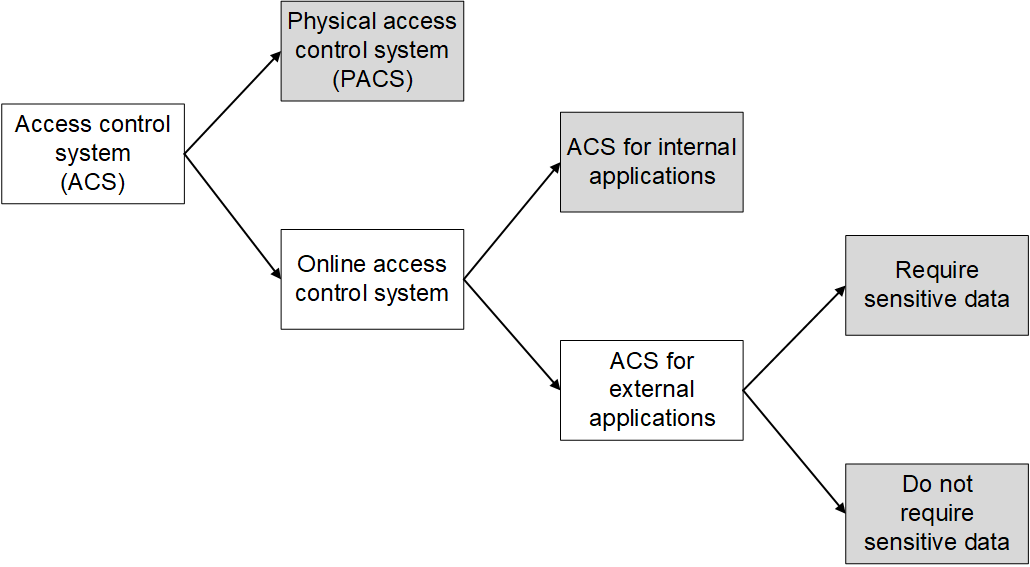
\includegraphics[width=.95\textwidth]{acs-classification}
    \caption{Access control system breakdown chart. \acrshort{acs} for external applications is different for applications work with sensitive data from \acrshort{acs} for external applications that do not work with sensitive data.}
    \label{fig:acs-classification}
\end{figure}

\subsection{Authentication}\label{sec:analysis-authentication}
In \acrshort{pacs}, physical tokens, such as ID cards, are the common practice nowadays. A survey carried out in 2016 indicated that above 40\% of the companies use low frequency proximity cards as their main method for personal authentication~\cite{HIDGlobal2017TheEnterprise}. These cards, operating in 125-134kHz frequency range are considered an obsolete technology and are not secure~\cite{Hakamaki2015SecurityTechnology}. On the other hand, around 20\% of the companies indicated use of mobile devices as a part of their \acrshort{pacs} solution~\cite{HIDGlobal2017TheEnterprise}. 

The main benefit of using a mobile device for this purpose is, that most people already own a smartphone and usually carry it with them at all times. Other technologies represented in the survey that are considered secure today, include iCLASS (contact-less card) and MIFARE DesFire (contact-less card). FIDO, nor FIDO2 keys (NFC, Bluetooth, or other) are not mentioned in the survey, although compatible \acrshort{pacs} systems exist on the market today\footnotemark. 

FIDO and FIDO2 enjoy support of big companies like Google, Facebook and Microsoft, but consumer-oriented services from these providers only permit the use of FIDO/FIDO2 as the second authentication factor. Google uses FIDO U2F keys for their employees, but only as a password replacement in the online login scenario~\cite{Krebs2018Google:Phishing} and Microsoft only supports FIDO2 keys with personal Microsoft accounts. As shown in Section~\ref{sec:online-access-control}, even Azure AD does not support this technology. To explore how FIDO2 can be used for hybrid access control on an enterprise scale, we propose the support of FIDO2 as a requirement for our system.
% 
\footnotetext{\url{https://web.archive.org/web/20190319221618/https://www.yubico.com/works-with-yubikey/catalog/modis/}, accessed 19 March 2019}

There is already a variety of devices that have been FIDO2 certified, with the Android system being a recent addition to the list~\cite{FIDOAlliance2019AndroidPasswords}. Considerations need to be put into how the FIDO2 flow is incorporated in the system and which of the FIDO2-certified devices are used in the flow. In the \acrshort{pacs} usability, namely the speed, is an important criteria, since existing systems already offer very low- to no-latency during a typical door opening use case. Beyond \acrshort{pacs}, the current access control solutions are mostly used for employee identification (as an ID badge)~\cite{HIDGlobal2017TheEnterprise} and the employee is only issued a single badge. The recommended approach in case the employee forgets the badge is to assign a temporary one that can be used during a limited time period and must be returned afterwards~\cite{Ryan2018HowBadges}.

In the online authentication, we can see that the systems support a wider range of authentication (and account recovery) methods, and the user is left to decide, which is authentication method do they prefer (see Section~\ref{sec:online-access-control}). Offering multiple methods simultaneously makes sense in the online access control scenario, because unlike in \acrshort{pacs}, where the on-site reception/security personnel can verify employees' identity and issue a temporary badge, in the online access control the identity verification is more complicated. In the case of forgotten credentials, the identity would therefore needed to be verified remotely (typically over phone), which is not feasible.

In the proposed hybrid access control system, it is desired to provide an authenticator, that is both fast to use and can be easily complemented and/or substituted with another authentication method if lost or forgotten. We propose the combination of FIDO2 key with \acrshort{nfc} as the primary authenticator, and FIDO2 enabled smartphone as the supplementary authenticator to meet the above criteria. The FIDO2 key with NFC support offers proximity-card-like usability (the user needs to swipe/hold the key next to the reader). If lost or forgotten, it can be substituted by an FIDO2 enabled smartphone, as people generally carry a smartphone with them, while at work. During our research, we have not encountered systems which offer the same selection of technologies, although the combination of a smartphone and an access card was seen in Section~\ref{sec:pacs-hid}.

% TODO FIDO2 would be used for all 4 boxes from access control breakdown chart

% TODO How OpenID connect is used for authentication/SSO
% TODO What information needs to be shared (Default OIDC scope - name, email, UID)...?
% TODO What entities will be needed (OID provider)
% TODO OpenID connect would be used only for boxes 3 and 4 from access control breakdown chart


% For \acrlong{aal}s 2 and 3 defined in 
% %  REFERENCE SECURITY REQUIREMENTS FOR CRYPTOGRAPHIC MODULES
% , authentication must be carried out using at least two independent factors. This requirement, together with abandonment of memorised secrets results in adoption of new authenticators. These  authenticators should offer at better security as memorised secrets, while maintaining the same level of accessibility. In 


\subsection{Authorisation}

When someone is authorise to use a system, it means they have permission to access that system. However, in enterprise access control scenario, there are other concepts associated with authorisation, rather than only verifying whether a user is allowed to use a certain system. The support for federated identity and the ability to handle \acrfull{sso} are typically design parameters that fall under the broader authorisation scope. Technologies that support these are discussed in the following section.

We can assume that an enterprise operates a variety of different IT systems, some of which may operate within the enterprise's security realm, while others may be \acrshort{saas} or may be operated by a business partner. To avoid an employee needing to manage several sets of credentials (one set for each system), federated identity is used. The access control system in an enterprise needs to be able to integrate with business application, so that federated identity can be used to access applications throughout the application landscape.

Once we acknowledge that a user should be able to use a single account (i.e. one set of credentials) to log in to both internal and external applications, we should further aim to reduce the number of times these credentials need to be entered, as the user logs into different systems, but without compromising the security of these systems. Single sign on addresses this need. With the single sign on, we could for example specify, that the user only needs to authenticate with their credentials once per two hours on a single machine. Once the user has authenticated, all the following requests to log in to any application using user's federated identity will be carried out without prompting the user to authenticate again, until the time limit has expired. This increases the convenience for the user.

Several technologies on the market support this approach. The most prominent ones, which we consider further are \acrshort{saml} and the OAuth + \acrshort{oidc} combination. Business applications that support federated identity integration, tend to support at least one of these technologies. While we could not find statistics comparing the use of the two in enterprises, we found examples of applications supporting both \acrshort{saml} and OAuth + \acrshort{oidc} and examples of applications that only support \acrshort{saml} (see Appendix~\ref{sec:appendix-links} for details). 

By some, \acrshort{saml} is considered as the enterprise-oriented technology, while OAuth and \acrshort{oidc} are considered oriented on the consumer market~\cite{Fagbemi2016ComparingWS-Federation, SoftwareSecured2016Differentiating2, OneLoginInc.SAMLOAuth}. However, OAuth and \acrshort{oidc} have been published 7 and 9 years  (respectively) after \acrshort{saml}. It is therefore understandable, that \acrshort{saml} is still widely present in the enterprise market. However, both technologies can be used in an enterprise environment, as noted by~\cite{Naik2017SecuringConnect} and some even encourage the use of OAuth + \acrshort{oidc} as the preferred way for new applications~\cite{barbkess2019SingleDirectory}.

Advantages of \acrshort{saml} include speed, identity-provider-initiated \acrshort{sso} and wide adoption~\cite{OneLoginInc.SAMLOAuth, Naik2017SecuringConnect}. The weaknesses are the limited support for mobile/native applications and heavy weight of the protocol (due to XML)~\cite{Naik2017SecuringConnect}. Conversely, the advantages of OAuth in combination with \acrshort{oidc} include better support for mobile and native applications, and more light-weight and REST-friendly protocol~\cite{Naik2017SecuringConnect}. There exists a proposal to improve the speed of OAuth in an enterprise setting~\cite{Noureddine2011AEnterprise}.

Because of better suitability for mobile and native applications, we propose OAuth + \acrshort{oidc} as the primary choice of authorisation and \acrshort{sso} protocols for internal enterprise applications and for external applications that support these technologies. Naturally, the system is likely to be integrated with internal legacy applications and external applications that do not support OAuth + \acrshort{oidc} for \acrshort{sso}. While a solution was proposed to enable OAuth functionality on legacy systems via \acrfull{esb}, this is not yet widely adopted and requires integration of an \acrshort{esb}~\cite{deSousaRibeiro2018AnBus}. Therefore the system should also support the \acrshort{saml} flow to accommodate these legacy systems.



% maybe-TODO Which scopes need to be included
% maybe-TODO Which entities will be needed to support this (Authorisation server)

% maybe-TODO OAuth will be used for boxes 3 and 4 from access control breakdown chart

\subsection{Access Policy Management}\label{Access_Policy_Management_Analysis}

In every \acrlong{acs}, the model used for granting the access play a crucial role as the system is dependent on it. Often it makes it easier for the administrator to manage and grant the access to employees, but if wrong model is chosen or is wrongly implemented, it can make the work even more burdensome. As it was outlined in the State of the Art (Chapter \ref{SOTA}), we are looking into \acrshort{rbac} and \acrshort{abac} as models for Identity and Access Management as they are the most used ones these days~\cite{2018BestV3}.

Both models offer a range of functionality and suits specific enterprises. One of \acrshort{rbac}’s big advantages is the ease of creating and maintaining the roles and system as a whole, but as the enterprise grows and more roles and resources are introduced, it gets complicated and hard to have an overview. Therefore, \acrshort{rbac} is suitable for small to medium enterprises. It is less complex than \acrshort{abac} and therefore it offers low level of granularity. Permission only can be granted to roles, not to operations or objects. On-the-fly contextual decisions are not supported, as well as restrictions can only be applied to parts of the system, not on specific data. Also, only known parameters can be used during implementation and environmental restrictions cannot be implemented. Even though, \acrshort{rbac} is older model it still offers adequate functionality.

On the other hand, \acrshort{abac} model which is based on attributes and policies presents fine grain and multi-dimensional access control. Biggest advantages of \acrshort{abac} over \acrshort{rbac} are the scalability of the model, dynamic parameters, easy maintenance and support for on-the-fly context aware decisions as information about requesting subject, requested object and environmental attributes are present. This way it is possible to grant access to specific data at specific times based on location. Initial configuration of the system is more complex compared to \acrshort{rbac}, but once done, it is easy to add new attributes or policies which are automatically executed. 

As the focus of the project, is to offer \acrlong{acs} to big enterprises, allowing fine grain control over resources, \acrlong{abac} model is more suitable for the solution. The trend in the industry is to adopt \acrshort{abac} more and more, and Gartner predicts that \textit{``By 2020, 70\% of businesses will use attribute-based access control (\acrshort{abac}) to protect critical assets''}~\cite{GartnerGartnerPredictions}. Studies also shows, that \acrshort{abac} is the model which should be used by enterprises in the future, rather than \acrshort{rbac}~\cite{Fatima2016TowardsArgument}.

To implement \acrshort{abac} model, the standard have to chosen as well. The most wide-spread standard is \acrshort{xacml}, which is explained in Section \ref{sec:xacml}, but others such as \acrfull{alfa} or \acrfull{ngac} exists as well. \acrshort{alfa} is a pseudocode language based on \acrshort{xacml} which provide higher user-friendliness, lower complexity and overall similar performance~\cite{Mejri2016FormalPolicies}. \acrshort{ngac} on the other hand, even-though it uses \acrshort{abac} model for access control, its implementation differs from \acrshort{xacml}~\cite{Ferraiolo2016ANGAC}. For the purpose of this project, we decide and propose the use of \acrshort{xacml} as the standard for implementing \acrshort{abac} in the system, mainly because of its wide spread, similar functionality to \acrshort{ngac} and the fact that it is being taught at the Identity and Access Management course at the university.
% \pagebreak
% \section{System Design}\label{sec:design}

The technologies and requirements identified previously are used in this chapter to design and propose a solution to the access control problem. First, the entities required to implement the system are listed. Due to resource limitations of this project, not all of the use cases that constitute the \acrshort{mvp} can be implemented. Instead, a subset of the use cases is selected to be implemented in the experimental prototype. These use cases are elaborated on in detail. Towards the end of this chapter, the system flows during authentication, policy evaluation and policy enforcement are described using sequence diagrams.

\subsection{Components}\label{sec:design-components}
To best design the architecture of the system, we must first understand the different actors and their roles. In the FIDO2, OAuth and \acrshort{oidc} specifications there is a degree of ambiguity -- problem being, that while each specification explains details in its own context, the link to other parts of an \acrshort{acs} are not obvious. In this section we identify components of our system and clear this ambiguity by drawing the borders of each specification within our system.

The external and internal systems are represented jointly as a \textit{Requester}. Requester is a system that is attempting to sign the user in, or access the protected resource. At the core of the proposed system is an \textit{\acrfull{aaserver}}, which carries out most of the authentication and authorisation tasks. The \acrshort{aaserver} consults with the User Directory and the  \acrfull{pdp}. To aid external systems retrieve information about users, the UserInfo endpoint translates the requests from the external systems to User Directory queries. Similarly, the Resource Endpoint provides access to the internal protected resources for the external systems. Both the UserInfo Endpoint and the Resource Endpoint are accessible from the public internet and lie on the boundary of the online security perimeter.

Figure~\ref{fig:data-flow-diagram} presents the high-level view of these components and their interactions. In the next sections we describe these components in more detail.

\begin{figure}[ht]
    \centering
    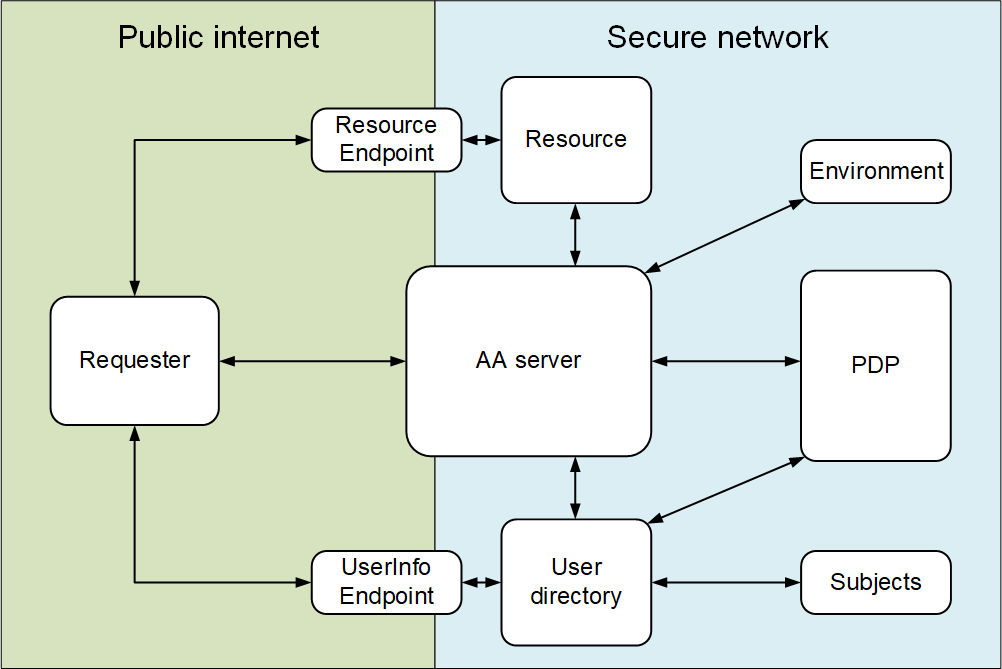
\includegraphics[width=.85\textwidth]{data-flow-diagram}
    \caption{High-level overview of system components and their interactions. The left side of the figure represents unsecured, public internet. The right side represents the security perimeter of the enterprise, which is not accessible from the public internet.}
    \label{fig:data-flow-diagram}
\end{figure}

\subsubsection{Requester} 
Requester is the system or application that is requesting access to protected resources on behalf of the user. Typically, this would be an internal or external client application, or a \acrshort{pacs}.

Client application is the business application the user wishes to use. If this is an internal application, it sits within the security perimeter and has direct access to the protected resources. However, it still needs to authenticate the user and verify that the user is authorised to access these resources.

If the client application is is an external application, it also typically requires that the user is authenticated and is authorised to use this application. Furthermore, it may require access to user's own resources on their behalf (e.g. user's files) and access to enterprise-owned resources on it's own behalf (e.g. list of departments).
    
The client application can be either of the three client types that are recognised by the OAuth specification~\cite{Hardt2012TheFramework} -- web-based application (running on a web server), user-agent-based application (downloaded from the web server, but executed locally) or a native application. Examples of client application are Slack, Salesforce, ServiceNow or Zendesk.

The \acrshort{pacs} can also be a requester. Similarly as an internal application, it sits within the security perimeter. It needs to authenticate the users and evaluate whether the user is authorised to pass beyond a certain point in a facility.

\subsubsection{User agent}
User agent does not act on its own, but instead hosts web-based and user-agent-based applications. It interacts with the user during login and authentication by displaying login forms and communicating with the physical authenticator device via the CTAP2 protocol\footnotemark. It is typically a web browser. Principally, it could be both desktop- and mobile-based (currently only on the Android mobile platform). 
% 
\footnotetext{In the FIDO2 terminology, the user agent would be called the \textit{client} or \textit{client device}.}

Examples of user agents are Chrome, Mozilla, Microsoft Edge.

\subsubsection{Authentication and Authorisation Server} 
The \acrfull{aaserver} is the core of the proposed access control system. As the name suggests, it handles the authentication and authorisation of the users. It communicates with the User Agent, the Requester, the User Directory and the \acrshort{pdp}.
    
\paragraph{User access request}
The \acrshort{aaserver} authenticates the user during sign in, before they can use the client application, or during physical access control. This flow is activated by a \textit{User access request} from the Requester. If the Requester is a client application, the \acrshort{aaserver} supplies a login form. If the Requester is a \acrshort{pacs}, the login form is omitted to increase the speed of the process. The \acrshort{aaserver} then communicates with the Requester, the User Directory and, optionally with the Authentication front end until the user has been authenticated (this communication is described in detail in Section~\ref{sec:access-control-flows}).

After authentication, the \acrshort{aaserver} proceeds to verify that the user is authorised to access the requested resource. It supplies the necessary information to the \acrshort{pdp} and receives a response with the policy decision.

If the OAuth + \acrshort{oidc} flow is required and the \acrshort{pdp} issued an `Allow access' decision, the \acrshort{aaserver} continues the process with the requester until an access token and/or ID token are issued. If the \acrshort{pdp} issued a `Deny access' decision, the \acrshort{aaserver} informs the Requester that the access has been denied and does not issue the access token or ID token. 

If the OAuth and \acrshort{oidc} are not required (when the requester is an internal application or a \acrshort{pacs}), the \acrshort{aaserver} simply forwards the policy evaluation decision to the requester.

\paragraph{Client access request}
When a Requester requires access to protected resources on its own behalf, the user authentication flow is skipped. Instead, the Requester begins the process by sending a \textit{Client access request} to the \acrshort{aaserver}. The client then authenticates using its own set of credentials, using the client credential grant type, as defined by~\cite{Hardt2012TheFramework}. 

The \acrshort{aaserver} verifies the access policy for the Requester and if the Requester is authorised to access the protected resources, it issues an access token.

The client access request can only be sent by a web-based client (which runs on a server), since native and user-agent-based clients cannot guarantee the security of the client credentials.

\bigskip \noindent
Example of a similar system is Azure AD, discussed in Section~\ref{sec:online-access-control} or ForgeRock Identity Platform\footnotemark.
% 
\footnotetext{\url{https://www.forgerock.com/resources/view/63280622/product-brief/forgerock-identity-platform.pdf}, accessed 10 April 2019.}
    
\subsubsection{Authentication Front End}
The Authentication front end is used during user authentication, when the user selects to authenticate using FIDO2 on a smartphone. The Authentication Front End is a middle layer between the \acrshort{aaserver} and the smartphone OS, which handles the CTAP2 protocol, and moderates the communication between these two parties.

It receives Authentication Assertions (as defined by~\cite{Balfanz2019Web1}) from the \acrshort{aaserver} and presents these to the smartphone OS, which handles the signing process. Once signed, the Authentication Front End returns the assertions to the \acrshort{aaserver}.

The Authentication Front End could be a native application, running directly on the smartphone OS, but could also be a web page, if the browser is capable of relying the Authentication assertions to the OS\footnotemark. In our proposed system, this is a webpage, to offer more convenient access from a smartphone (without installation).
% 
\footnotetext{For example Chrome on Android supports the use of WebAuthn and CTAP2~\cite{ChromePlatformStatus2018SupportAPI}.}

\subsubsection{User Directory}
The User Directory is a directory service that stores user attributes and can be accessed by the internal systems. In the proposed \acrshort{acs}, the User Directory is used to supply attributes about users for authentication and policy evaluation purposes. It also serves attributes to the UserInfo endpoint, when queried.

In addition to standard user attributes (such as name, email, office phone, job title etc.), the user directory stores details about user's authenticators -- the \texttt{credentialPublicKey}(as defined by~\cite{Balfanz2019Web1} -- authenticator's public key). This entry is created when the authenticator is first registered (UC-5) and is used to verify whether the credential challenge for a particular user was signed by an authenticator belonging to this user. Further authenticator details stored in the directory could be the signature counter or a user-defined authenticator name.

The User Directory interacts with the \acrshort{aaserver} when it supplies authenticator challenges and verifies authenticator challenge responses. It further interacts with the \acrshort{pdp} where it supplies user attributes, if these are required by the \acrshort{pdp} to evaluate the policy.

Examples of a user directory would be Active Directory\footnote{Active Directory by Microsoft is a subset of Azure AD described in Section~\ref{sec:online-access-control} on page~\pageref{sec:online-access-control}.} or the Apache Directory\footnotemark.
% 
\footnotetext{\url{https://web.archive.org/web/20190407171447/https://directory.apache.org/}, accessed 07 April 2019.}
    
\subsubsection{Policy Decision Point}
The \acrfull{pdp} determines whether a given user or Requester is authorised to access a protected resource. The \acrshort{pdp} stores the policies and when queried by the \acrshort{aaserver}, it evaluates the relevant policy and issues an evaluation decision.

It evaluates the policy based on user/Requester attributes, and optionally, additional context information. Some of these attributes are supplied by the \acrshort{aaserver} in the query. If these attributes are not sufficient to evaluate a policy, the \acrshort{pdp} can request additional information from the User Directory or the \acrshort{aaserver}.

As specified by RQ-22, \acrshort{xacml} is used to evaluate access policies. The \acrshort{pdp}, described by the \acrshort{xacml} specification~\cite{OASISStandard2013EXtensible3.0}, cannot operate on its own. Instead it communicates with other components to enforce the policy on the requester. The mapping of the proposed system components to the \acrshort{xacml} context is illustrated in Figure~\ref{fig:xacml-use}, Appendix~\ref{sec:xacml-use} on page~\pageref{fig:xacml-use}.

Example of a solution that implements \acrshort{pdp} functionality is \href{sec:online-access-control}{Azure AD} or WSO2 Identity Server\footnotemark.
% 
\footnotetext{\url{https://web.archive.org/web/20190407180021/https://docs.wso2.com/display/IS570/WSO2+Identity+Server+Documentation}, accessed 07 April 2019.}
    
\subsubsection{Resource Endpoint}
The Resource Endpoint serves the external clients. This endpoint is the gateway for the external application to access the protected enterprise resources. These resources are divided into scopes and the client must present a valid access token for the scope it is attempting to access. The endpoint must verify the validity of the presented token, before it serves the resource. The scopes are defined as \acrshort{api}s, specifying the form of the request and response messages.
    
\subsubsection{UserInfo Endpoint}
The UserInfo endpoint is a component as defined in~\cite{Sakimura2014Final:1}. It serves claims about user attributes to the external clients. The client must present a valid access token to receive the attributes of the associated user. The UserInfo Endpoint serves as an access point for clients outside the security perimeter, but it does not store any user attributes itself. Instead, it queries the User Directory for any requested attributes every time such request is received.

\bigskip \noindent
Not all of the mentioned components are necessarily different physical entities, but we list them here separately as they perform a different functions and are logically independent. In the Section~\ref{sec:access-control-flows} we describe some of the interactions between these components.
\subsection{Prototype Use Cases} \label{sec:design-prototype-usecases}
To demonstrate the functionality of the proposed \acrshort{acs} in practice, we select the most common uses of our system: signing in, passing a checkpoint and accessing a protected resource. These are represented by UC-1, UC-2, and UC-16 and are discussed further.

UC-1 and UC-2 include the authentication flow with FIDO, which is not used widely today in the combination of Online and \acrlong{pacs}, as discussed in Section~\ref{sec:analysis-authentication}. UC-16 (generalisation of UC-17 and UC-18) complements the sign-in process by providing information about the user and serving the protected resources to the client. These are essentially the use cases that an employee would encounter on a daily basis. The remaining use cases are more administrative and are not necessary to demonstrate the intended system functionality, therefore they are not discussed further.

On the following pages, detailed description of the use cases is provided for UC-1 (Table~\ref{tab:useCase_01}), UC-2 (Table~\ref{tab:useCase_02}), UC-17 (Table~\ref{tab:useCase_10}) and UC-18 (Table~\ref{tab:usecase-18-specs}).

\newgeometry{left=1.2cm,right=1.2cm,top=1cm,bottom=1cm,footskip=.4cm}
\begin{table}[htpb!]
    \footnotesize
    \onehalfspacing
    \centering
    \begin{tabular}{|c|p{15cm}|}
    \hline
    \cellcolor[HTML]{CBCEFB}\textbf{Name}&
    UC-1: Sign-in to a system
    \\
    \hline
    \cellcolor[HTML]{CBCEFB}\textbf{Description}&
    Employee signs-in to an internal or external client system with their enterprise digital identity using single-factor \acrshort{fido} physical key via \acrshort{usb} or \acrshort{nfc}; or \acrshort{fido} on a smartphone.
    \\
    \hline
    \cellcolor[HTML]{CBCEFB}\textbf{Primary actors}& 
    \textbullet~Employee
    \\
    \hline
    \cellcolor[HTML]{CBCEFB}\textbf{Secondary actors}& 
    \textbullet~Internal system, or \newline
    \textbullet~External system
    \\
    \hline
    \cellcolor[HTML]{CBCEFB}\textbf{Pre-conditions}&
    \vspace{-\topsep}
    \begin{itemize}[nolistsep, noitemsep, leftmargin=*]
        \item Employee has an enterprise digital identity assigned.
        \item Employee has previously registered at least one of the following authenticators:
        \begin{enumerate*}[label=(\roman*)]
            \item single-factor \acrshort{fido} physical key with \acrshort{usb} or \acrshort{nfc},
            \item \acrshort{fido} enabled smartphone.
        \end{enumerate*}
        \item Employee is in control of the previously registered authenticator.
        \item Employee does not have an active session with the given client on the given device.
        \item Policies have been set up that authorise the employee to access the client.\vspace*{-\baselineskip}
    \end{itemize}
    \\
    \hline
    \cellcolor[HTML]{CBCEFB}\textbf{Processing}& 
    \vspace{-\topsep}
    \begin{enumerate}[nolistsep, noitemsep, leftmargin=*]
        \item Employee launches the client application (either natively on the platform or in a web-browser). The client can be either internal system or external system. The sign-in process of the employee is the same in both cases. 
        \item Employee clicks on \textit{Sign-in}, \textit{Log-in} or similar button, or is redirected to sign-in automatically. A sign-in form appears.
        \item Employee enters their \acrlong{uid}.
        \item Employee is prompted to select their preferred authentication method: a physical key or a smartphone. If a physical key is selected, the employee is prompted to use their key with their device (depending on the make of the key and the device). If a smartphone is selected, the employee is prompted to navigate to a predefined website (enterprise-supplied authentication front end) on their smartphone, where they are prompted to authenticate with FIDO.
        \item Once the employee has been successfully authenticated, their attributes are checked against the existing policies for the system and the authorisation to access the system is verified.\vspace*{-\baselineskip}
    \end{enumerate}
    \\
    \hline
    \cellcolor[HTML]{CBCEFB}\textbf{Outcome}& 
    \vspace{-\topsep}
    \begin{itemize}[nolistsep, noitemsep, leftmargin=*]
    \item Employee signed-in and may begin to use the system, or
    \item Employee is denied to access the system because they could not be authenticated or are not authorised to access the given system.\vspace*{-\baselineskip}
    \end{itemize}
    \\
    \hline
    \cellcolor[HTML]{CBCEFB}\textbf{Post-conditions}&
    \textbullet~A session is created between employee's device and the system. Depending on the security settings, the employee might not need to sign in the next time when they use the system.
    \\
    \hline
    \end{tabular}
    \caption{Detailed specification of UC-1}
    \label{tab:useCase_01}
\end{table}
% 
% 
% 
% 
% 
\begin{table}[htpb!]
    \footnotesize
    \onehalfspacing
    \centering
    \begin{tabular}{|c|p{15cm}|}
    \hline
    \cellcolor[HTML]{CBCEFB}\textbf{Name}& 
    UC-2: Pass through a physical checkpoint
    \\
    \hline
    \cellcolor[HTML]{CBCEFB}\textbf{Description}& 
    Employee authenticate themselves to \acrlong{pacs} with their enterprise digital identity, using a \acrshort{fido} physical key via \acrshort{nfc} or with \acrshort{fido} on their smartphone.
    \\
    \hline
    \cellcolor[HTML]{CBCEFB}\textbf{Primary actors}&
    \textbullet~Employee
    \\
    \hline
    \cellcolor[HTML]{CBCEFB}\textbf{Secondary actors}&
    \textbullet~\acrlong{pacs}
    \\
    \hline
    \cellcolor[HTML]{CBCEFB}\textbf{Pre-conditions}&
    \vspace{-\topsep}
    \begin{itemize}[nolistsep, noitemsep, leftmargin=*]
        \item Employee has an enterprise digital identity assigned.
        \item Employee has previously registered at least one of the following authenticators:
         \begin{enumerate*}[label=(\roman*)]
            \item single-factor \acrshort{fido} physical key with \acrshort{usb} or \acrshort{nfc},
            \item \acrshort{fido} enabled smartphone.
         \end{enumerate*}
         \item Policies have been set up that authorise the employee to pass the given checkpoint.\vspace*{-\baselineskip}
     \end{itemize}
    \\
    \hline
    \cellcolor[HTML]{CBCEFB}\textbf{Processing}&
    \vspace{-\topsep}
    \begin{enumerate}[nolistsep, noitemsep, leftmargin=*]
        \item Employee approaches the checkpoint and the \acrshort{pacs} reader device mounted in vicinity.
        \item Employee swipes their physical FIDO key at the reader device to identify and authenticate themselves; or
        \item Employee indicates at the reader device that they wish to use smartphone to identify and authenticate themselves. They visit a special website (enterprise-supplied authentication front end), where they input the checkpoint ID and then authenticate using FIDO on the smartphone. 
        \item Once the system has authenticated the employee, it checks whether the policy permits the employee to pass the given checkpoint.\vspace*{-\baselineskip}
    \end{enumerate}
    \\
    \hline
    \cellcolor[HTML]{CBCEFB}\textbf{Outcome}&
    \vspace{-\topsep}
    \begin{itemize}[nolistsep, noitemsep, leftmargin=*]
    \item The checkpoint allows the employee to pass through, if the authentication was successful and policy permits access; or
    \item The access is denied and the employee is informed about the denial.\vspace*{-\baselineskip}
    \end{itemize}
    \\
    \hline
     \cellcolor[HTML]{CBCEFB}\textbf{Post-conditions}&\textbullet~Access attempt is logged in the system logs.\\
     \hline
    \end{tabular}
    \caption{Detailed specification of UC-2}
    \label{tab:useCase_02}
\end{table}
% 
% 
% 
% 
% 
\begin{table}[htpb!]
    \footnotesize
    \onehalfspacing
    \centering
    \begin{tabular}{|c|p{15cm}|}
    \hline
    \cellcolor[HTML]{CBCEFB}\textbf{Name}&
    UC-17: Access user's protected resources 
    \\
    \hline
    \cellcolor[HTML]{CBCEFB}\textbf{Description}&
    External systems might need to read or modify user's protected resources, such as files, emails, calendar entries, or others, to fulfil their function.
    \\
    \hline
    \cellcolor[HTML]{CBCEFB}\textbf{Primary actors}&
    \textbullet~External client
    \\
    \hline
    \cellcolor[HTML]{CBCEFB}\textbf{Secondary actors}&
    None
    \\
    \hline
    \cellcolor[HTML]{CBCEFB}\textbf{Pre-conditions}&
    \vspace{-\topsep}
    \begin{itemize}[nolistsep, noitemsep, leftmargin=*]
        \item A client connection between the external system and the \acrshort{acs} has been established.
        \item The policy permits the system to access user's protected resources.
        \item The user has previously signed in to the external system.\vspace*{-\baselineskip}
    \end{itemize}
    \\
    \hline
    \cellcolor[HTML]{CBCEFB}\textbf{Processing}&
    \vspace{-\topsep}
    \begin{enumerate}[nolistsep, noitemsep, leftmargin=*]
        \item The \acrshort{acs} verifies that the external system has been registered and has been assigned a client ID.
        \item The \acrshort{acs} verifies that the user is signed in or has previously singed in to the external system. This can be demonstrated with a refresh token.
        \item The \acrshort{acs} verifies that the policy permits the external system to access user's protected resources.
        \item If the previous conditions are met, the \acrshort{acs} issues an access token to the External client. The external client uses this token when querying the system for user's resources. The validity of the token is time bound and can be only used to request resources about the user it has been issued for.\vspace*{-\baselineskip}
    \end{enumerate}
    \\
    \hline
    \cellcolor[HTML]{CBCEFB}\textbf{Outcome}&
    \vspace{-\topsep}
    \begin{itemize}[nolistsep, noitemsep, leftmargin=*]
    \item The external system can read or modify user's resources, after it has successfully presented a valid access token; or
    \item Access was denied and the external system cannot manipulate user's protected resources.\vspace*{-\baselineskip}
    \end{itemize}
    \\
    \hline
     \cellcolor[HTML]{CBCEFB}\textbf{Post-conditions}&
     \textbullet~The access token cannot be used for other user's resources, or after it's validity has expired.
     \\
     \hline
    \end{tabular}
    \caption{Detailed specification of UC-17}
    \label{tab:useCase_10}
\end{table}
% 
% 
% 
% 
% 
\begin{table}[htpb]
    \footnotesize
    \onehalfspacing
    \centering
    \begin{tabular}{|c|p{15cm}|}
    \hline
    \cellcolor[HTML]{CBCEFB}\textbf{Name}&
    UC-18: Access enterprise protected resources
    \\
    \hline
    \cellcolor[HTML]{CBCEFB}\textbf{Description}&
    External systems might need to read or modify protected resources owned by the enterprise (and which are not owned by any single user) to fulfil their function.
    \\
    \hline
    \cellcolor[HTML]{CBCEFB}\textbf{Primary actors}&
    \textbullet~External system
    \\
    \hline
    \cellcolor[HTML]{CBCEFB}\textbf{Secondary actors}&
    None
    \\
    \hline
    \cellcolor[HTML]{CBCEFB}\textbf{Pre-conditions}&
    
    \vspace{-\topsep}
    \begin{itemize}[nolistsep, noitemsep, leftmargin=*]
        \item A client connection between the external system and the \acrshort{acs} has been established and a client secret has been issued to the external system.
        \item The client acting on behalf of the external system is web-server based.
        \item The policy permits the access to the protected resources.\vspace*{-\baselineskip}
    \end{itemize}
    \\
    \hline
    \cellcolor[HTML]{CBCEFB}\textbf{Processing}&
    \vspace{-\topsep}
     \begin{enumerate}[nolistsep, noitemsep, leftmargin=*]
        \item The \acrshort{acs} verifies the client's client ID and client secret.
        \item The \acrshort{acs} verifies that the policy permits the external system to access enterprise protected resources.
        \item If the conditions are met, the \acrshort{acs} issues an Access Token to the External system client. The client presents this access token, when it is manipulating the protected resources. The access token has a limited validity and cannot be used for any other than requested resources, or after it's validity period has elapsed.\vspace*{-\baselineskip}
     \end{enumerate}
    \\
    \hline
    \cellcolor[HTML]{CBCEFB}\textbf{Outcome}&
    \vspace{-\topsep}
    \begin{itemize}[nolistsep, noitemsep, leftmargin=*]
        \item The external client obtained an access token and presented it in the request to manipulate the protected resource; or
        \item The external client has been denied access to the protected resources.\vspace*{-\baselineskip}
     \end{itemize}
    \\
    \hline
     \cellcolor[HTML]{CBCEFB}\textbf{Post-conditions}&
     \textbf~The access token cannot be used, after it's validity has expired.
     \\
     \hline
    \end{tabular}
    \caption{Detailed specification of UC-18}
    \label{tab:usecase-18-specs}
\end{table}
\restoregeometry
\subsection{Prototype Requirements}\label{sec:design-prototype-requirements}

Based on the use cases highlighted in the previous section, we describe the requirements necessary to implement these use cases. Naturally, all requirements linked with given use cases should be implemented. The following requirements are linked to the selected use cases: RQ-1, RQ-2, RQ3, RQ-4, RQ-5, RQ-18 and RQ-19. These requirements are selected to be implemented in the prototype and drive the design choices behind the system architecture. 

% TODO describe selected Requirements

% \begin{table}[H]
%     \footnotesize
%     \onehalfspacing
%     \centering
%     \begin{tabular}{|c|p{15cm}|}
%     \hline
%     \cellcolor[HTML]{CBCEFB}\textbf{ID}&\cellcolor[HTML]{CBCEFB}\textbf{Description}\\
%     \hline
%     RQ-1&User must be able to authenticate with single-factor cryptographic device based on FIDO2 to use their enterprise digital identity.\\
%     \hline
%     RQ-2&User must be able to authenticate with smartphone using FIDO2 flow to use their enterprise digital identity.\\
%     \hline
%     RQ-4&User must be able to sign-in to external client system with their enterprise digital identity.\\
%     \hline
%     RQ-5&User must be able to open a door with their enterprise digital identity.\\
%     \hline
    %     % RQ-19&\textbf{External client system must be able to access protected resources, when authorised to do so.}\\
%     RQ-18&External client system must be able to access protected resources if permission granted.\\
%     \hline
%     RQ-19&External client system must be able to obtain grant permission.\\
%     \hline
%     \hline
%     RQ-20&Authentication to PACS using enterprise digital identity must be comparably fast to traditional RFID access cards (order of milliseconds to seconds).\\
%     \hline
%     % RQ-21&\textbf{External system must be able to access protected resources.}\\
%     % \hline
%     RQ-21&The system must use OIDC + OAuth for Authentication and Authorisation.\\
%     \hline
%     RQ-22&The system must use XACML for Identity and Access management\\
%     \hline
%     \end{tabular}
%     \caption{List of functional requirements \#1, \#2, \#4, \#5, \#18, \#19 and non-functional requirements \#20, \#21, \#22 for the prototype.}
%     \label{tab:prototype-requirements}
% \end{table}
\subsection{Access control flows}
% NAME? "System flow example(s)

The access control flow of the proposed system can be broken down into three stages:
\begin{enumerate*}[label=(\roman*)]
    \item \textit{Authentication},
    \item \textit{Access Policy Evaluation} and
    \item \textit{Accessing protected resource}.
\end{enumerate*}
These stages can be identified in every use case of the system, although the flow in each stage is adapted to the given use case.

\subsubsection{Authentication}
In this stage, the user identifies and authenticates themselves to the \acrshort{aaserver}. This is the first stage of the access control flow and is only preceded by the user clicking a login button or approaching a door. The authentication is done via the FIDO2 protocol, but the flows during this stage are different during online login and when opening a door.

\paragraph{Authenticating online} During online authentication the user uses a browser or a native client application to communicate with the \acrshort{aaserver}. When the user clicks a login button, the client application redirects them to the login page, supplied by the \acrshort{aaserver}. The user agent/native client application needs to send a `Access request' message to the server, which contains these parameters: the \texttt{client\_id}, the callback URL, the requested scopes (and if the client is a native application, also the \acrshort{pkce} code challenge). The \texttt{client\_id} is immediately verified by the \acrshort{aaserver}. All variables are temporarily saved for use later in the process. 

The \acrshort{aaserver} provides a login form back to the requesting party. User enters their \acrshort{uid} into this form and chooses the authenticator they wish to use (physical key or smartphone). The filled form is then send back to the \acrshort{aaserver}. The server requests a login challenge for this \acrshort{uid} from the User directory. The User directory looks up the \acrshort{uid} in the user database and generates an Authentication assertion\footnotemark to be signed by the user's authenticator.
% 
\footnotetext{As defined by the WebAuthn specification: \url{https://www.w3.org/TR/webauthn/\#dictdef-publickeycredentialrequestoptions}, accessed 08 April 2019}

If the user selected physical key as their authenticator, the Authentication assertion is then forwarded back to the user agent/native application that made the initial access request. If the user selected smartphone, the the Authentication assertion is forwarded to the Authentication front end. Once the signed assertion is received, the \acrshort{aaserver} forwards it to the User directory. User directory verifies that the signature was made by either of the public keys, associated with the \acrshort{uid}. The User directory then informs the \acrshort{aaserver} about the outcome of this verification. 

In the last step of the Authentication stage, the \acrshort{aaserver} issues a signed and encrypted \acrshort{jwt} to the user agent/Authentication front end. This \acrshort{jwt} can be sent in the initial Access request and the remaining steps of the authentication stage are then skipped. The purpose of this is to avoid repeated authentication prompts to the user in a short time span (a couple of hours). Once the user authenticates using an authenticator on certain user agent, we do not need to prompt authentication on the same user agent again, until the validity of the \acrshort{jwt} has expired.

If a \acrshort{aaserver} receives a valid \acrshort{jwt} in the Access request, it does not carry out further authentication steps and proceeds directly to the Access policy evaluation stage. If the received \acrshort{jwt} is expired or otherwise invalid, the regular process described above applies.

\subsubsection{Access Policy Evaluation}

*tune of pink panther*
TO DO, TODO, TODO, TODO, TODOOOO....
% \pagebreak
% \section{Implementation}
Implementation to be written

% TODO write implementation
% \pagebreak
% \section{Discussion}\label{sec:discussion}
In this chapter we discuss the progress and the outcomes of the prototype implementation. We then consider several open problems that were not covered in this project, but are relevant for launch of a combined access control system on the market. Possible ways of performing multi-factor authentication are examined, followed by considerations about the future development of FIDO and its implementations. Lastly, potential future works that could extend and built on top of the system are discussed.

\subsection*{Implementation}
In Chapter~\ref{sec:design} we identify a number of use cases and requirements that should be implemented in the prototype to demonstrate the functionality of the system. During the implementation work it was confirmed that there is ongoing work on the different parts of the access control problem in the general coding community. This was demonstrated by the existence of numerous active repositories, libraries and guides for FIDO, OAuth and OIDC.

Despite existence of these, we were not able to implement all of the use cases set out for the prototype. A possible reason for this is the recentness of the involved technologies, mainly FIDO/Webauthn. While the specifications exists and are adopted by major browsers, there is still some degree of ambiguity among existing implementations in the ``gray'' areas not covered by the specification, such as how to store the data in a database, how to parse data to prepare them for transport, or what encoding version (\texttt{Base64} vs \texttt{Base64Url}) should be predominantly used.

In the OAuth/OIDC space, a lot of focus is put into integrating new applications with existing OAuth providers (implementing sign-in with Facebook, Google and similar). In commercial applications, it is not desired to implement own sign-in system and convergence towards the major providers can be seen. However, as demonstrated in the prototype, it is still possible to deploy a customised OAuth/OIDC Authorisation Server.

Even though the prototype does not implement all of the selected use cases, we find it valuable as it does demonstrate some of the fundamental flows of authentication and access policy enforcement. Further work on implementation would gradually resolve the existing issues and present a working solution. To arrive at a marketable \acrshort{mvp}, integration with Active Directory and/or \acrshort{ldap} would need to be implemented in addition to the other \acrshort{mvp} requirements specified in Section~\ref{sec:analysis-requirements}.

\subsection{Multi-factor authentication considerations} \label{multiFA}

Multi-factor authentication is an approach where two or more factors for successful authentication of a user are required. This way, if one of factors is compromised, there is a need for compromising the other factors as well in order to successfully access the resources. \acrshort{nist} in their Digital Identity Guidelines~\cite{Grassi2017Digital3} specifies three groups of authenticators which can be used for authentication:
\begin{itemize}[noitemsep]
    \item Something you know (typically a password, \acrshort{pin}, etc.)
    \item Something you have (typically a physical cryptographic key, authenticator application, etc.)
    \item Something you are (typically a fingerprint, retina scan, etc.)
\end{itemize}

Choosing a right combination of authenticators is crucial for every system as it can either strengthen the security or if badly combined even weaken it. Therefore, now we will analyse each of these three groups of authenticators and suggest the most suitable one.

\paragraph{Something you know}
Authenticators from this group has been used for centuries, however in the era of technical advance and modern technologies they become obsolete and hard to manage. People are using dozens of services online for which they need to remember some kind of password or \acrshort{pin}. Therefore, they are often choosing easy to remember passwords or are using the same for all services~\cite{2018OnlineSurvey}. On top of that, passwords are prone to phishing attacks and it is possible a user will forget it. Furthermore, one of the aims of the system presented in this project, is to avoid the use of passwords. Using\textit{ ``something you know’’} as another factor would therefore go against our initial goal of not using this element.

\paragraph{Something you have}
In the enterprise environment, access cards (RFID or proximity cards) are used often, this is just one factor authentication thought. These days, there are many options for authentication using \textit{``something you have’’}, some being more user friendly than the others. It is popular to use a phone to receive a SMS or an email with a \acrfull{otp} to prove identity, but it has been advised by NIST not to use it anymore~\cite{NIST2017NISTBlog}. For the purposes of our system, as mentioned before (in section \ref{sec:analysis-authentication}), we are planning to use a physical cryptographic key to authenticate a user as a primary authentication method, instead of \textit{``something you know’’}. Using two physical cryptographic keys is not advised because of a high chance of losing them both at the same time. On the other hand, using \acrshort{otp} generator such as smartphone application or smart card is feasible, because of its simplicity, ease of use and price. 

\paragraph{Something you are}
People tend to forget and lose things; therefore, one can argue that using \textit{``something you are’’} is the most user friendly and secure of all above mentioned authenticators. Fingerprint scan is among the most used authenticators. FIDO2 which is implemented in our system has been certified on Android smartphones and biometric scanners can be used to authenticate users. Another option is to integrate fingerprint scanner to a physical cryptographic key. This way, the ownership of the device and identity of the user can be verified at the same time. Also, it fulfils the NIST requirement about using Biometrics in \acrshort{mfa}: \textit{Biometrics SHALL be used only as part of multi-factor authentication with a physical authenticator (something you have).}~\cite{Grassi2017DigitalManagement}. Both of these options are suitable for our enterprise scenario and can be proposed to be used.

\paragraph{Suggested solution}
Each of the authenticator types has it pros and cons. The most important criteria for choosing another factor in \acrshort{mfa} are the security and ease of use. Based on analysis above, three candidate solutions are found:
\begin{itemize}[noitemsep]
    \item \acrshort{otp} generator in form of calculator or smartphone application
    \item \acrshort{fido}2 physical cryptographic key with fingerprint scanner
    \item \acrshort{fido}2 certified smartphone with fingerprint scanner
\end{itemize}
All three solution are secure~\cite{Grassi2017DigitalManagement}, \cite{FIDOFIDO2Project}, fairly easy to use and can be implemented to our system. Our preference are both options containing FIDO2 as it is being implemented in the system already. However, as \acrshort{mfa} is not part of the requirements neither for \acrshort{mvp} nor for prototype, we will not go further in analyzing which of candidate solutions is the most feasible to implement.
\subsubsection*{FIDO considerations}
Shortly before this project was submitted, support of FIDO was announced by Windows as another major operating system, following Android~\cite{Mehta2019WindowsPasswordless}. This is a clear sign of growing support of password-less login scenarios. While both mobile and desktop devices included support for biometric sign-in to the OS for a number of year, this technology was not typically used outside the OS login and to log in to a limited number of native applications that implemented the OS specific libraries for integration with the biometric devices on the device.

FIDO2 helps by removing the need for direct OS integration by exposing the CTAP2 protocol to any interested party via Webauthn. While FIDO2 in itself is not directed at biometric authentication, it brings forward an important abstraction layer to enable secure, yet convenient password-less log-in experience, whether the authenticator is a physical cryptographic key, or the device itself with integrated biometric capabilities. This abstraction can be exploited in the proposed system as well, at least for authenticating to an Online Access Control System.
\subsubsection*{Coupling}
Section~\ref{sec:design-components} defines a number of individual components in the system, each component responsible for it's own, narrow task. A \acrshort{pdp} (only) evaluates policies, a User Directory (only) answers queries about users and the UserInfo endpoint only serves information about users to the external systems. This design represents a \textit{loosely coupled} system, where each module focuses only on its own task and is independent from its neighbours.

An alternative designed to the proposed system could be a single heavy-weight endpoint -- such as \acrshort{aaserver} -- that would take tasks of authenticating users, serving requests for user information and maybe even serving requests for protected resources. The advantages for external (and internal) applications would be that only a single endpoint is called at all times. Furthermore, only this single endpoint would be exposed to requests from the public internet, thus reducing the risks of security breach.

On the other hand, this approach suffers from the known disadvantages of tight coupling. The the single endpoint would be subject to bigger load and would need to be more versatile, than many separated endpoints. Furthermore, shall an outage occur to this single endpoint, the entire system would be inoperable, similarly, an update to a single functionality would require the update of the whole system. Loosely coupled, individual endpoints do not suffer from these pains. We maintain that benefits of the loose coupling outweigh its shortcomings and it presents a better fit in the access control scenario.
\subsubsection*{Future works}
As described in the beginning of this chapter, further work is needed to implement the envisioned the prototype and to fully implement the proposed system. Existing work on physical access control solutions with a smartphone should be reviewed in greater detail, before implementing this part of the system in practice. 

As new platforms announce support for FIDO2, the system flows should be redesigned to provide native support for this development, which could potentially simplify some of the authentication flows. Similarly, the implementation will be possible with less effort as the libraries mature and common practices are established around the specifications.

With further development of the system, additional use cases would likely have to be derived, to complement the minimal functionality of the proposed \acrshort{mvp}. During the development, several of such use cases were discovered, for example external employee, who needs access to the enterprise internal resources. In such case the system would need to be adapted to support identity federation across enterprises.
% \pagebreak
\section{Conclusion}\label{sec:conclusion}
Conclusion to be written
% TODO write conclusion

% A number of challenges arose when working on the project. The most fundamental challenge was to understand how \acrshort{acs} works, to identify its main components and to learn about the current systems. Once the knowledge is acquired, the selection of right technologies was an important aspect, as there exists many technologies and standards which can be implemented in the proposed system and therefore, finding the most suitable one was of a big importance. This goes hand in hand with designing a system’s architecture from the scratch and figuring out how the chosen components and technologies can be interconnected to perform desired tasks, while keeping in mind the security and easiness of use.
\pagebreak

\printbibliography[heading=bibintoc]

\epigraph{Passwords are dead.}{Everyone, since 2004. \textit{\href{http://fidoserver.ml:8080/about.jsp}{fidoserver.ml:8080/about.jsp}}}

\pagebreak

\appendix
% \newgeometry{left=1cm,right=1cm,top=1cm,bottom=1cm,footskip=.4cm}
% \section{SAML and OAuth + OpenID Connect support in enterprise applications}\label{sec:appendix-links}

\paragraph{Zendesk} Only supports SAML:

\url{https://support.zendesk.com/hc/en-us/articles/203663676}, accessed on 31 March 2019 (\href{https://web.archive.org/web/20190331182733/https://support.zendesk.com/hc/en-us/articles/203663676}{view archive version}).

\url{https://support.zendesk.com/hc/en-us/community/posts/115006523287-Does-Zendesk-Support-OpenID-Connect-}, accessed on 31 March 2019 (\href{https://web.archive.org/web/20190331182849/https://support.zendesk.com/hc/en-us/community/posts/115006523287-Does-Zendesk-Support-OpenID-Connect-}{view archive version}).

\paragraph{Slack} Only supports SAML:

\url{https://get.slack.help/hc/en-us/articles/203772216-SAML-single-sign-on}, accessed on 31 March 2019 (\href{https://web.archive.org/web/20190331183030/https://get.slack.help/hc/en-us/articles/203772216-SAML-single-sign-on}{view archive version}).

\paragraph{Salesforce} Supports both SAML and OAuth + OpenID Connect:

\url{https://help.salesforce.com/articleView?id=sso_saml.htm&type=5}, accessed on 31 March 2019 (\href{https://web.archive.org/web/20190331183852/https://help.salesforce.com/articleView?id=sso_saml.htm&type=5}{view archive version}).

\url{https://help.salesforce.com/articleView?id=sso_provider_openid_connect.htm&type=5}, accessed on 31 March 2019 (\href{https://web.archive.org/web/20190331184051/https://help.salesforce.com/articleView?id=sso_provider_openid_connect.htm&type=5}{view archive version}).

\paragraph{ServiceNow} Supports both SAML and OAuth + OpenID Connect:

\url{https://docs.servicenow.com/bundle/london-platform-administration/page/administer/security/task/add-OIDC-entity.html}, accessed on 31 March 2019 (\href{https://web.archive.org/web/20190331184433/https://docs.servicenow.com/bundle/london-platform-administration/page/administer/security/task/add-OIDC-entity.html}{view archive version}).

\url{https://docs.servicenow.com/bundle/london-platform-administration/page/integrate/saml/concept/c_SAML2.0WebBrowserSSOProfile.html}, accessed on 31 March 2019 (\href{https://web.archive.org/web/20190331184648/https://docs.servicenow.com/bundle/london-platform-administration/page/integrate/saml/concept/c_SAML2.0WebBrowserSSOProfile.html}{view archive version}).
% \newgeometry{left=1cm,right=1cm,top=1cm,bottom=1cm,footskip=.4cm}
% \section{XACML use comparison}\label{sec:xacml-use}

\begin{figure}[ht]
    \centering
    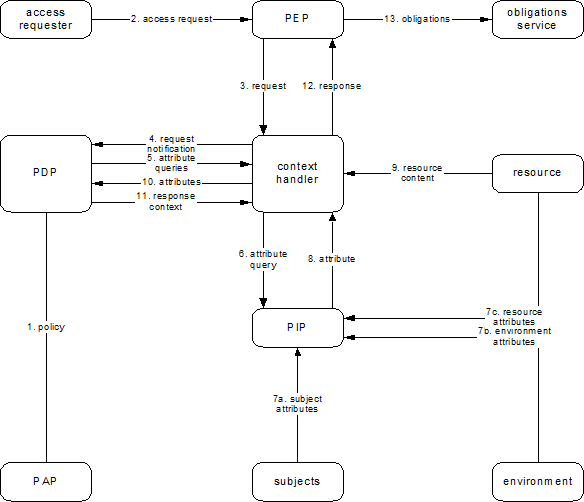
\includegraphics[width=\textwidth]{xacml-architecture}
    \caption{\acrshort{xacml} data flow diagram. Taken from~\cite{OASISStandard2013EXtensible3.0}.}
    \label{fig:xacml-architecture}
\end{figure}

\begin{sidewaysfigure}[ht]
    \centering
    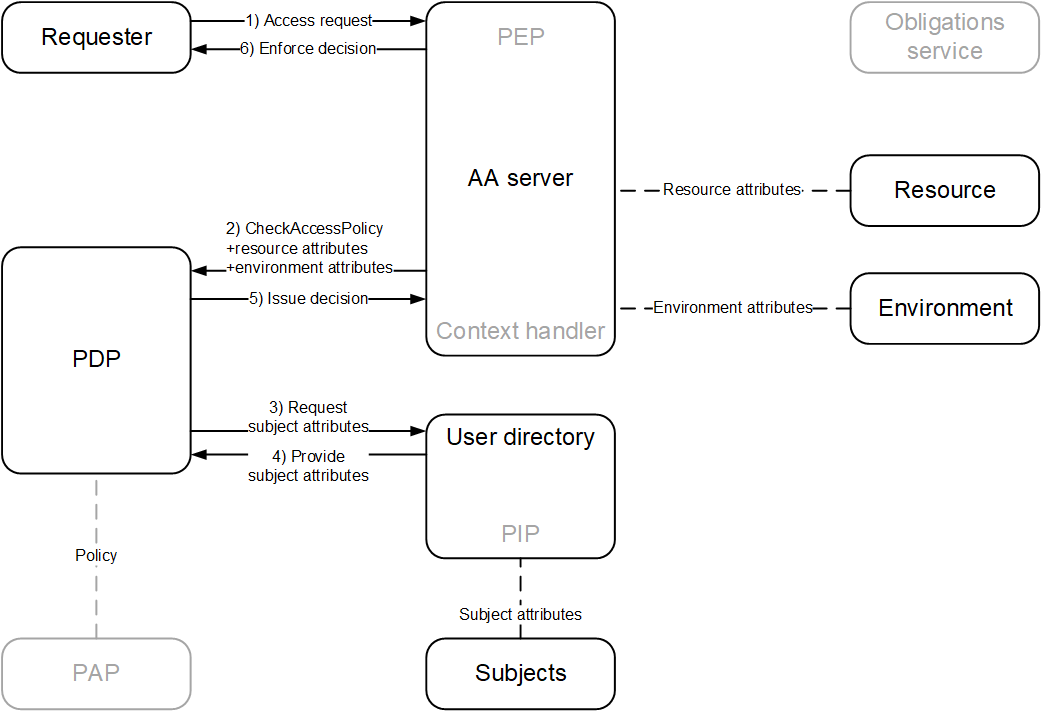
\includegraphics[width=.85\textwidth]{xacml-use}
    \caption{Data flow diagram of the proposed system. The parts in grey are not discussed in the report. In step two, the \acrshort{aaserver} supplies additional context information (resource and environment attributes) in its \texttt{CheckAccessPolicy} request. Furthermore, the \acrshort{aaserver} enforces the policy decision by issuing the access token if the policy evaluation is \textit{Allow access}, or by denying to issue the access token and returning an error message, if the evaluation decision is \textit{Deny access}.}
    \label{fig:xacml-use}
\end{sidewaysfigure}
% \newgeometry{left=2cm,right=2cm,top=1cm,bottom=1cm,footskip=.4cm}
% \section{Use Case Diagram}\label{sec:use-case-diagram}
% 
\begin{figure}[H]
    \centering
    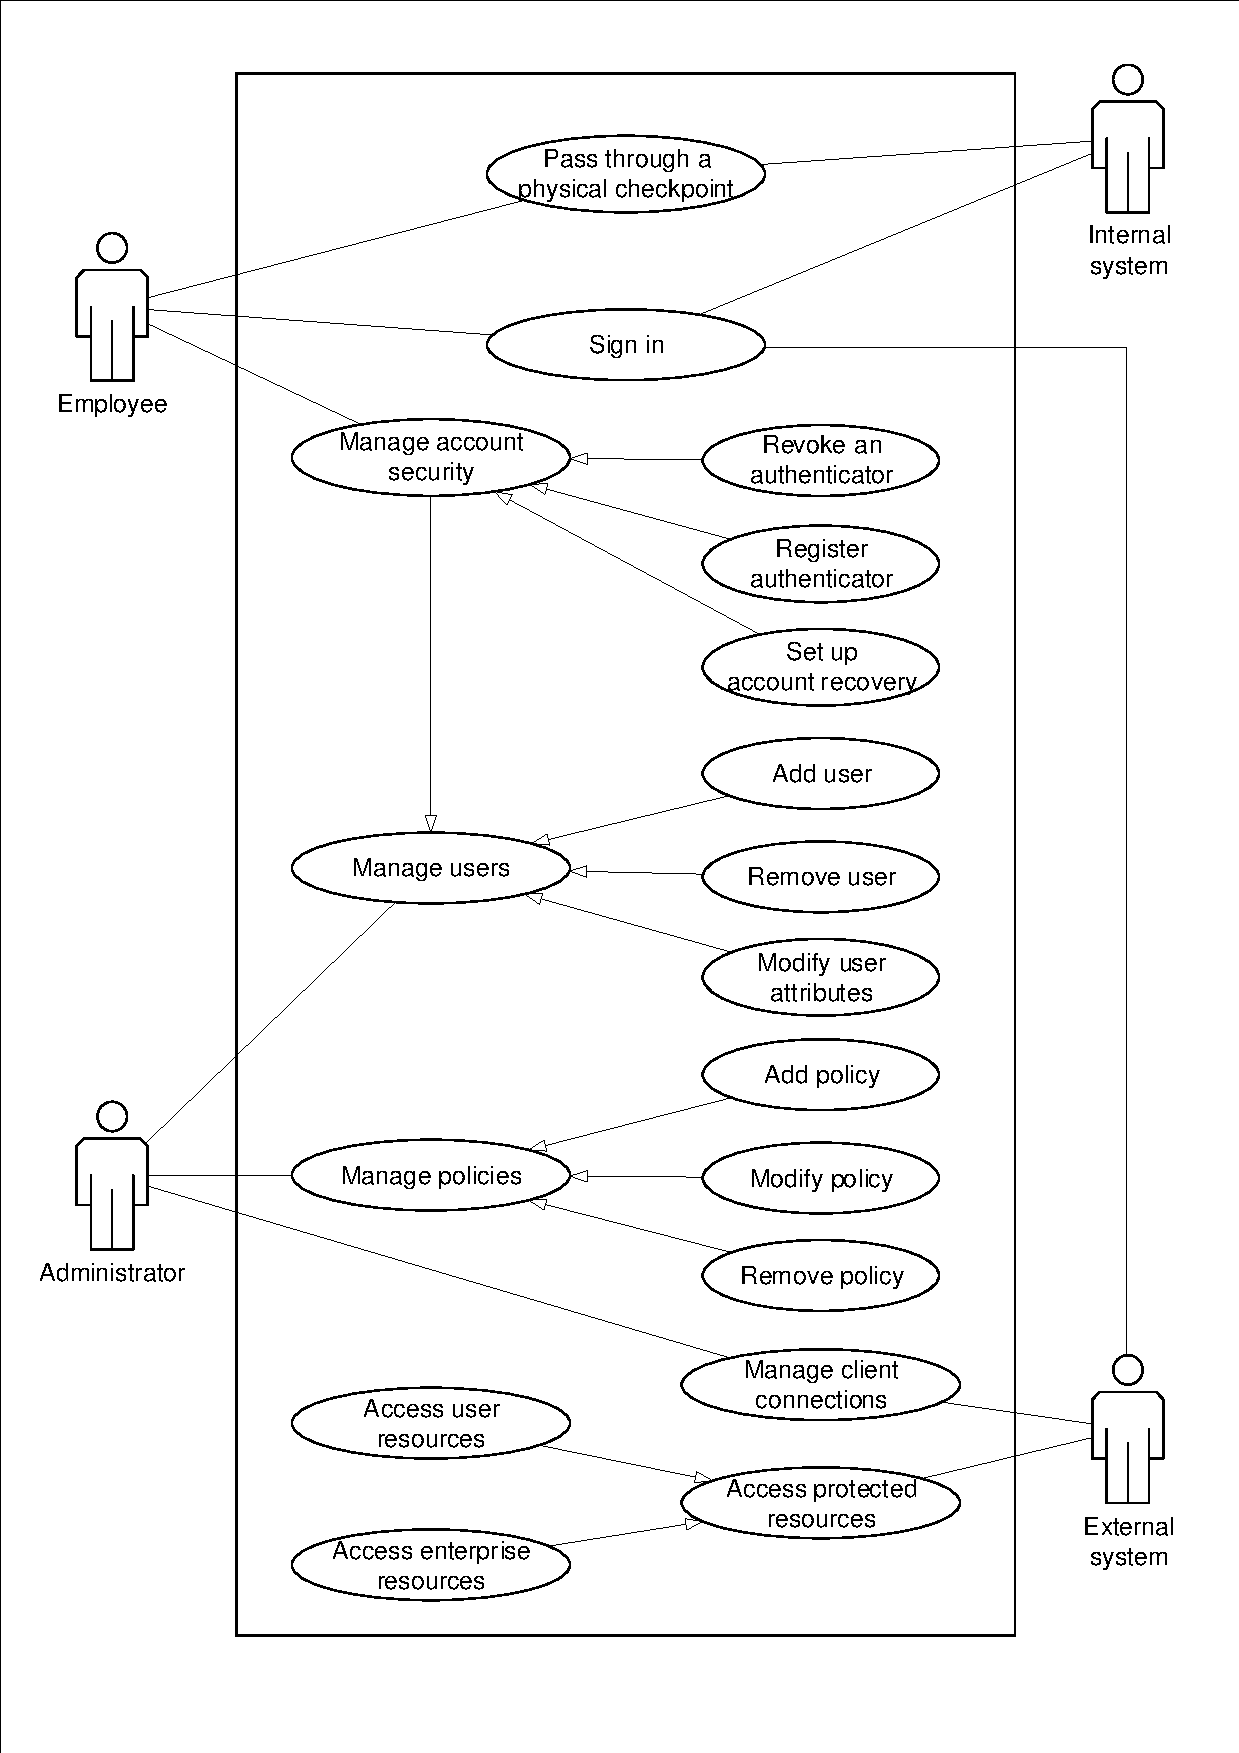
\includegraphics[height=.90\textheight]{use-cases}
    \caption{Use case diagram for the proposed \acrshort{acs} system.}
    \label{fig:use-case-diagram}
\end{figure}
% \newgeometry{left=1cm,right=1cm,top=1cm,bottom=1cm,footskip=.4cm}
% \begin{landscape}
\section{Additional sequence diagrams}\label{appendix:diagrams}
\subsection{Opening door with physical key}
% 
\begin{minipage}{\textwidth}
    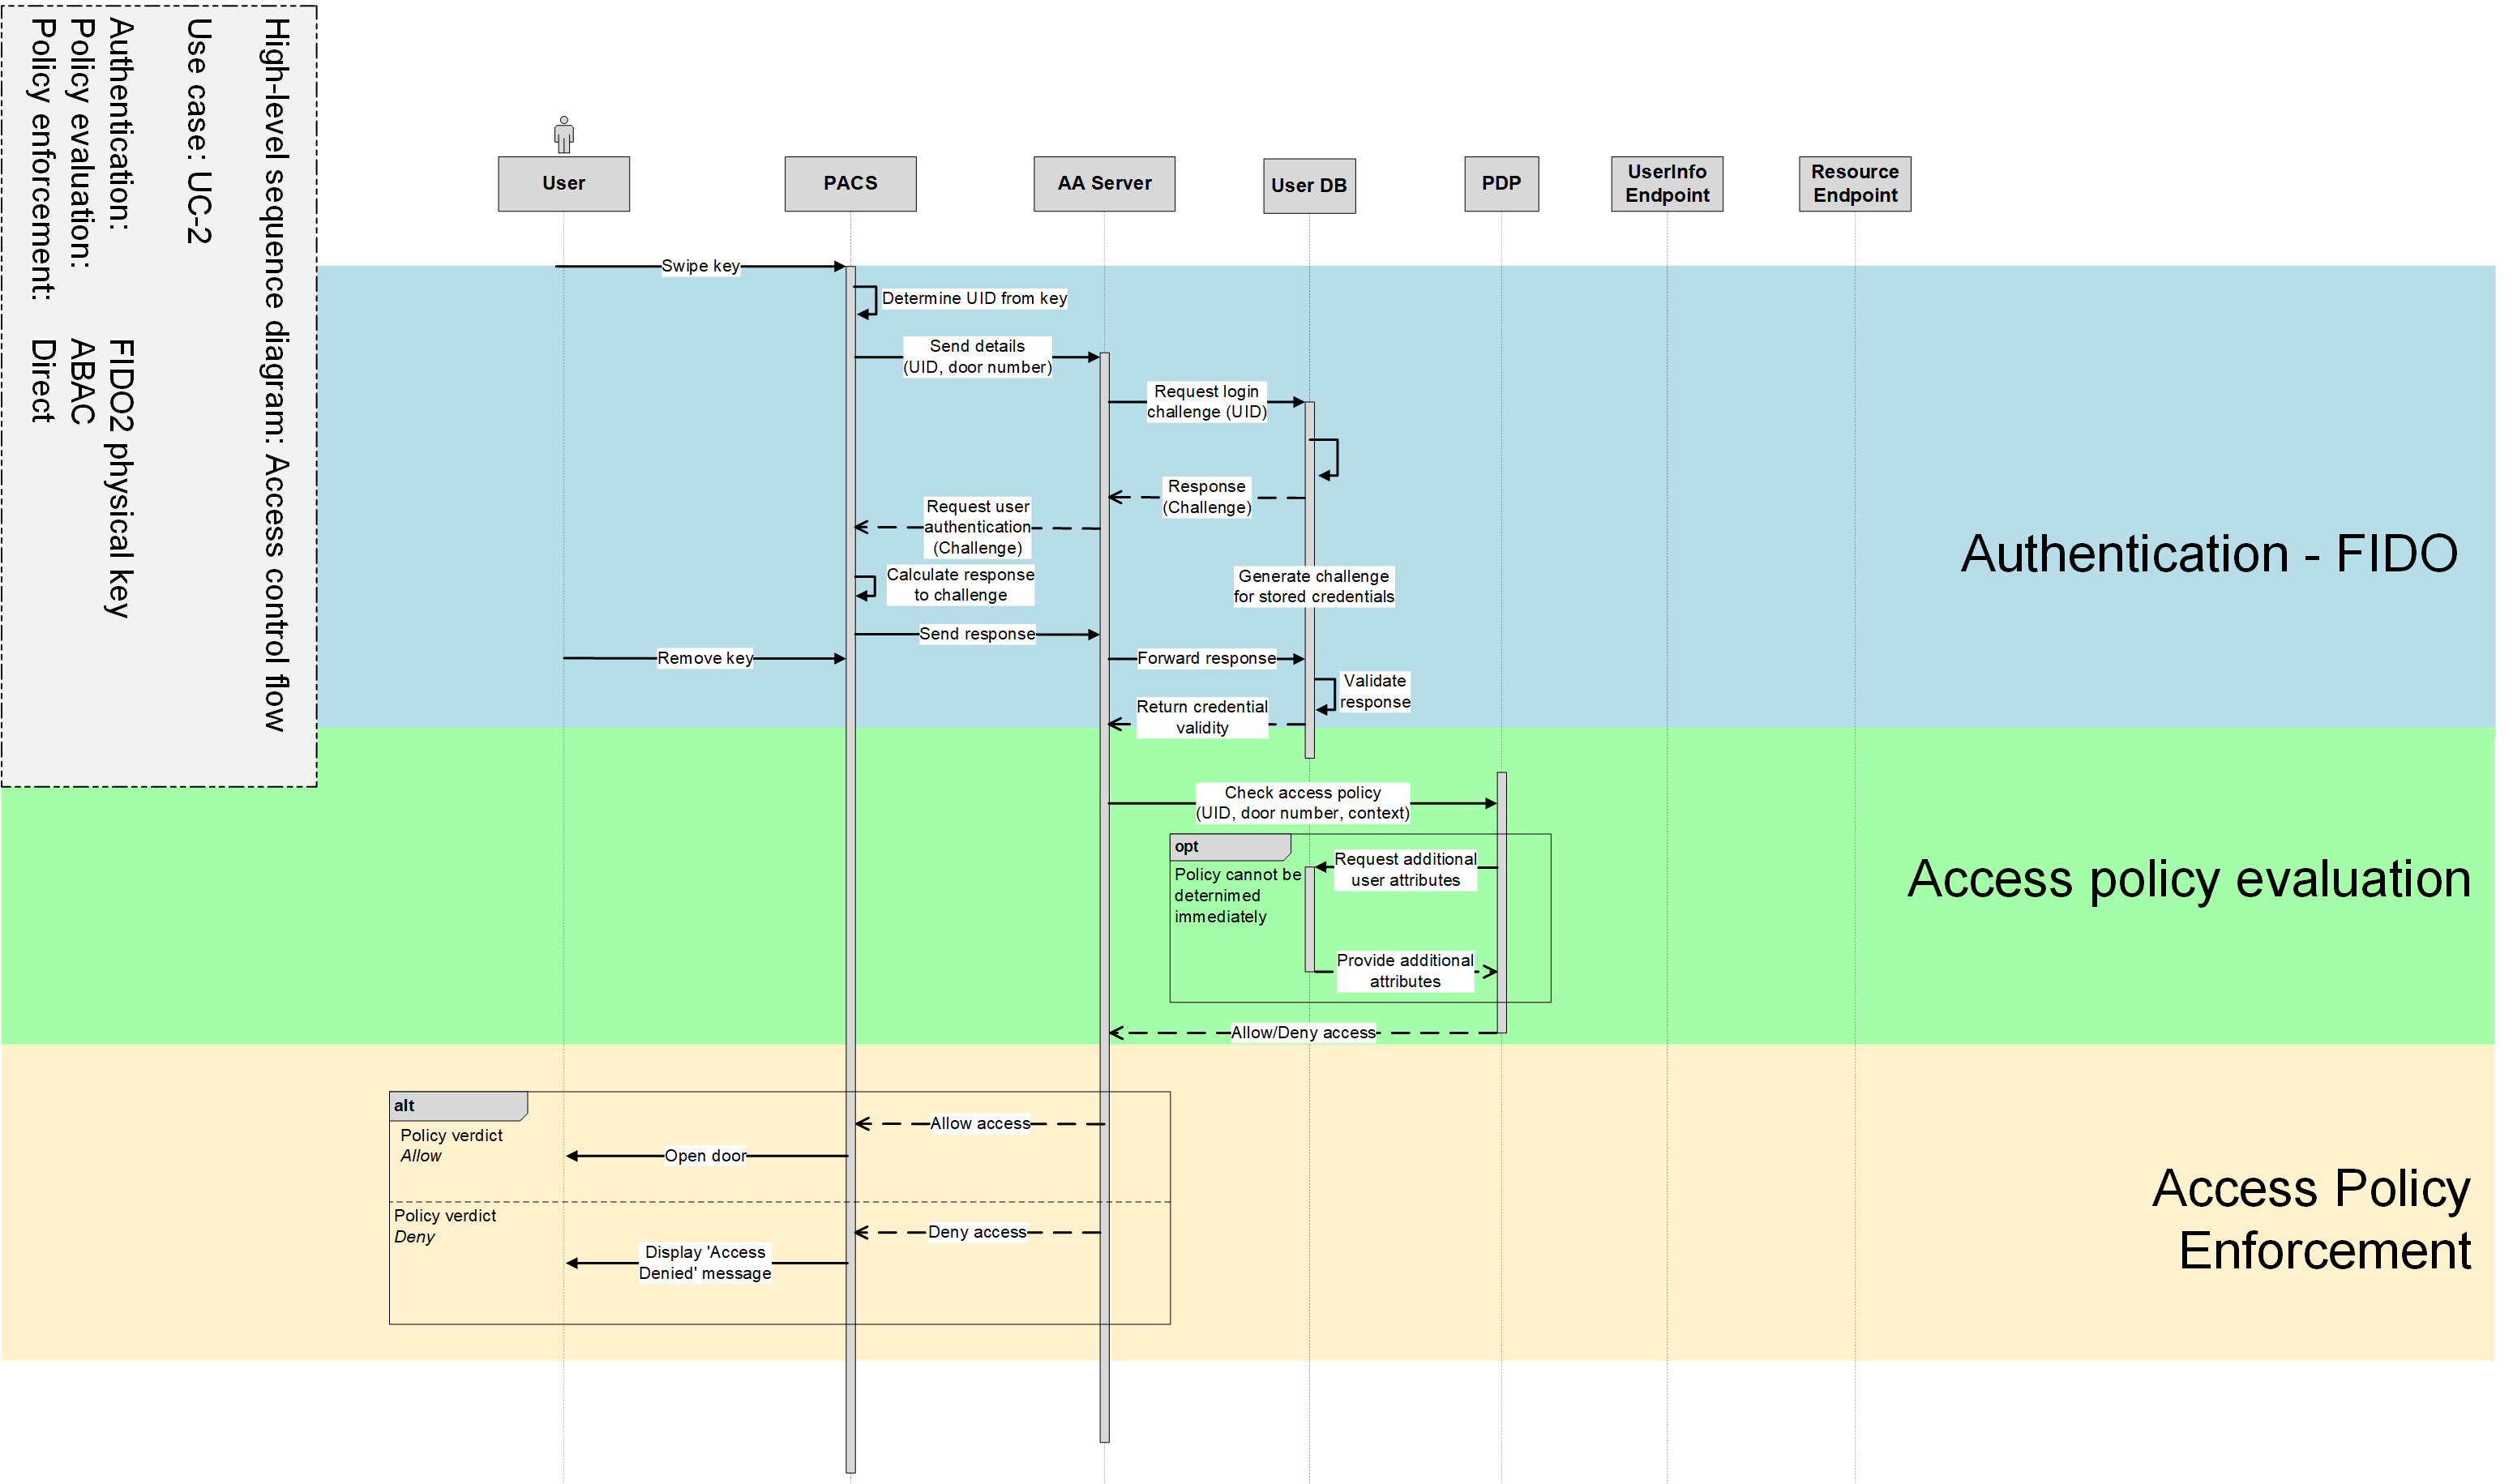
\includegraphics[width=1.25\textheight]{door-key-flow}
\end{minipage}
% 
\subsection{Opening door with a smartphone}
\begin{minipage}{\textwidth}
    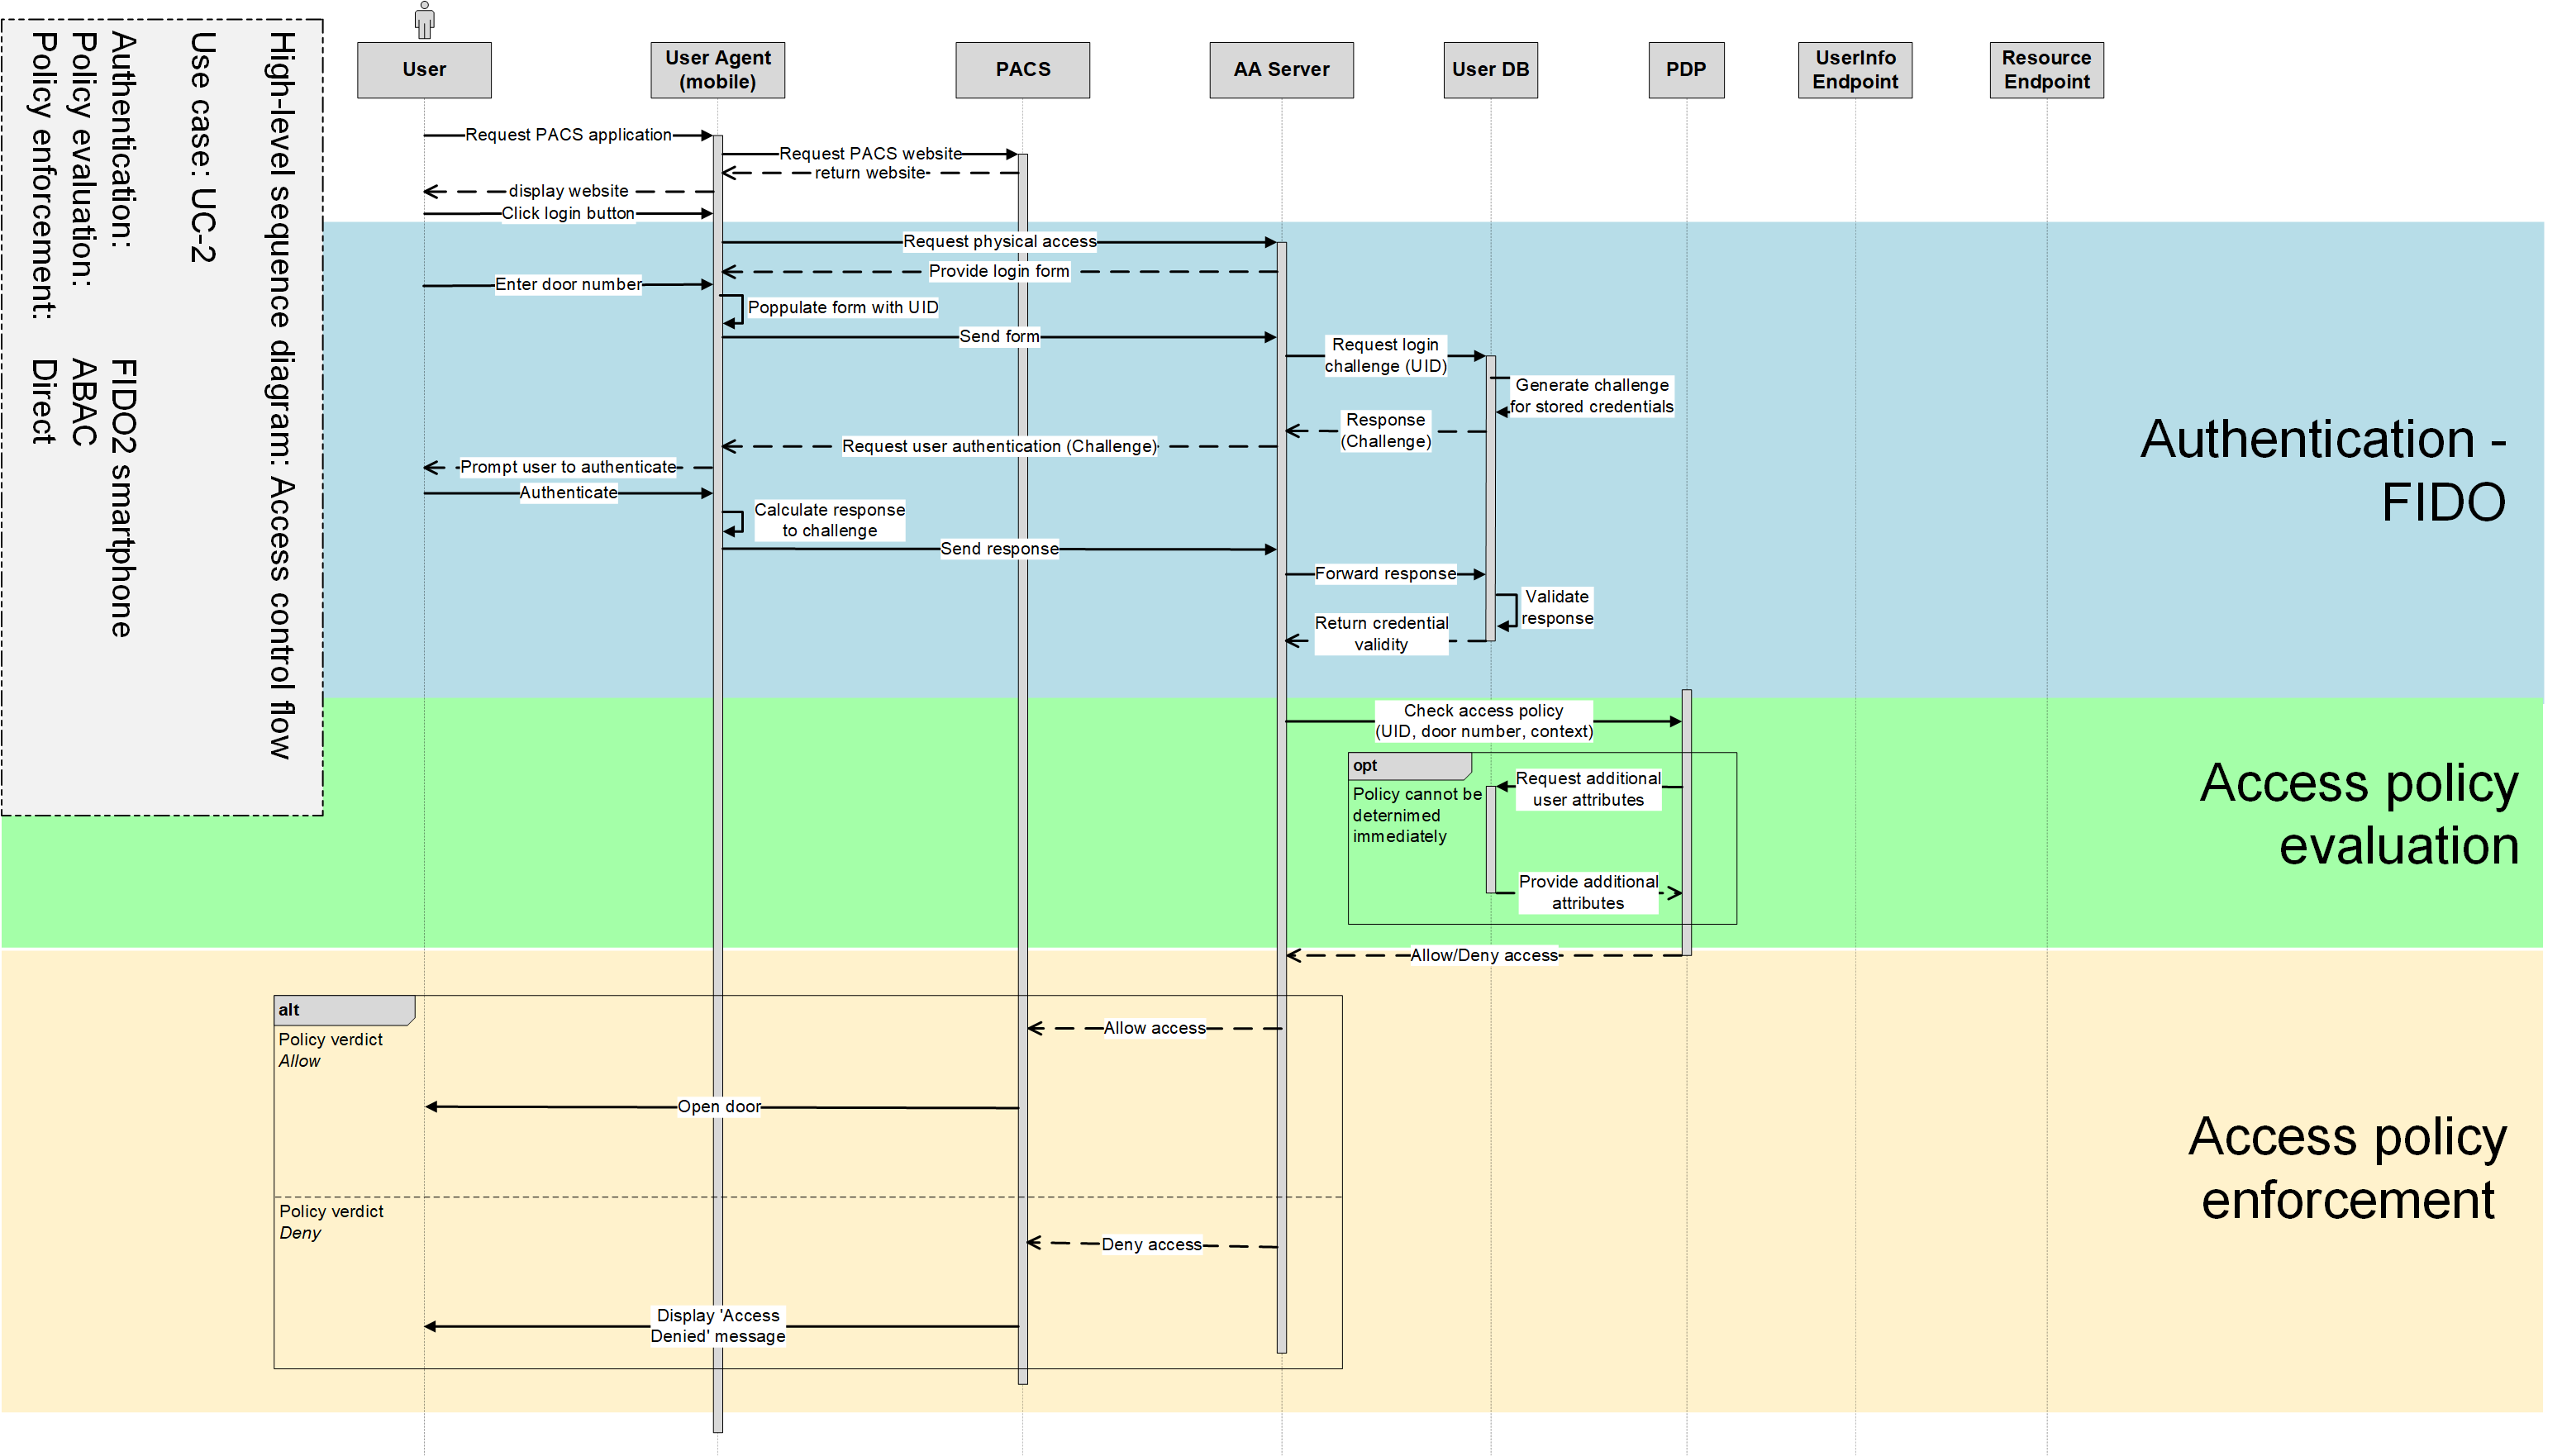
\includegraphics[width=1.35\textheight]{door-phone-flow}
\end{minipage}
% 
\subsection{Accessing an external online system with a native client}
\begin{minipage}{\textwidth}
    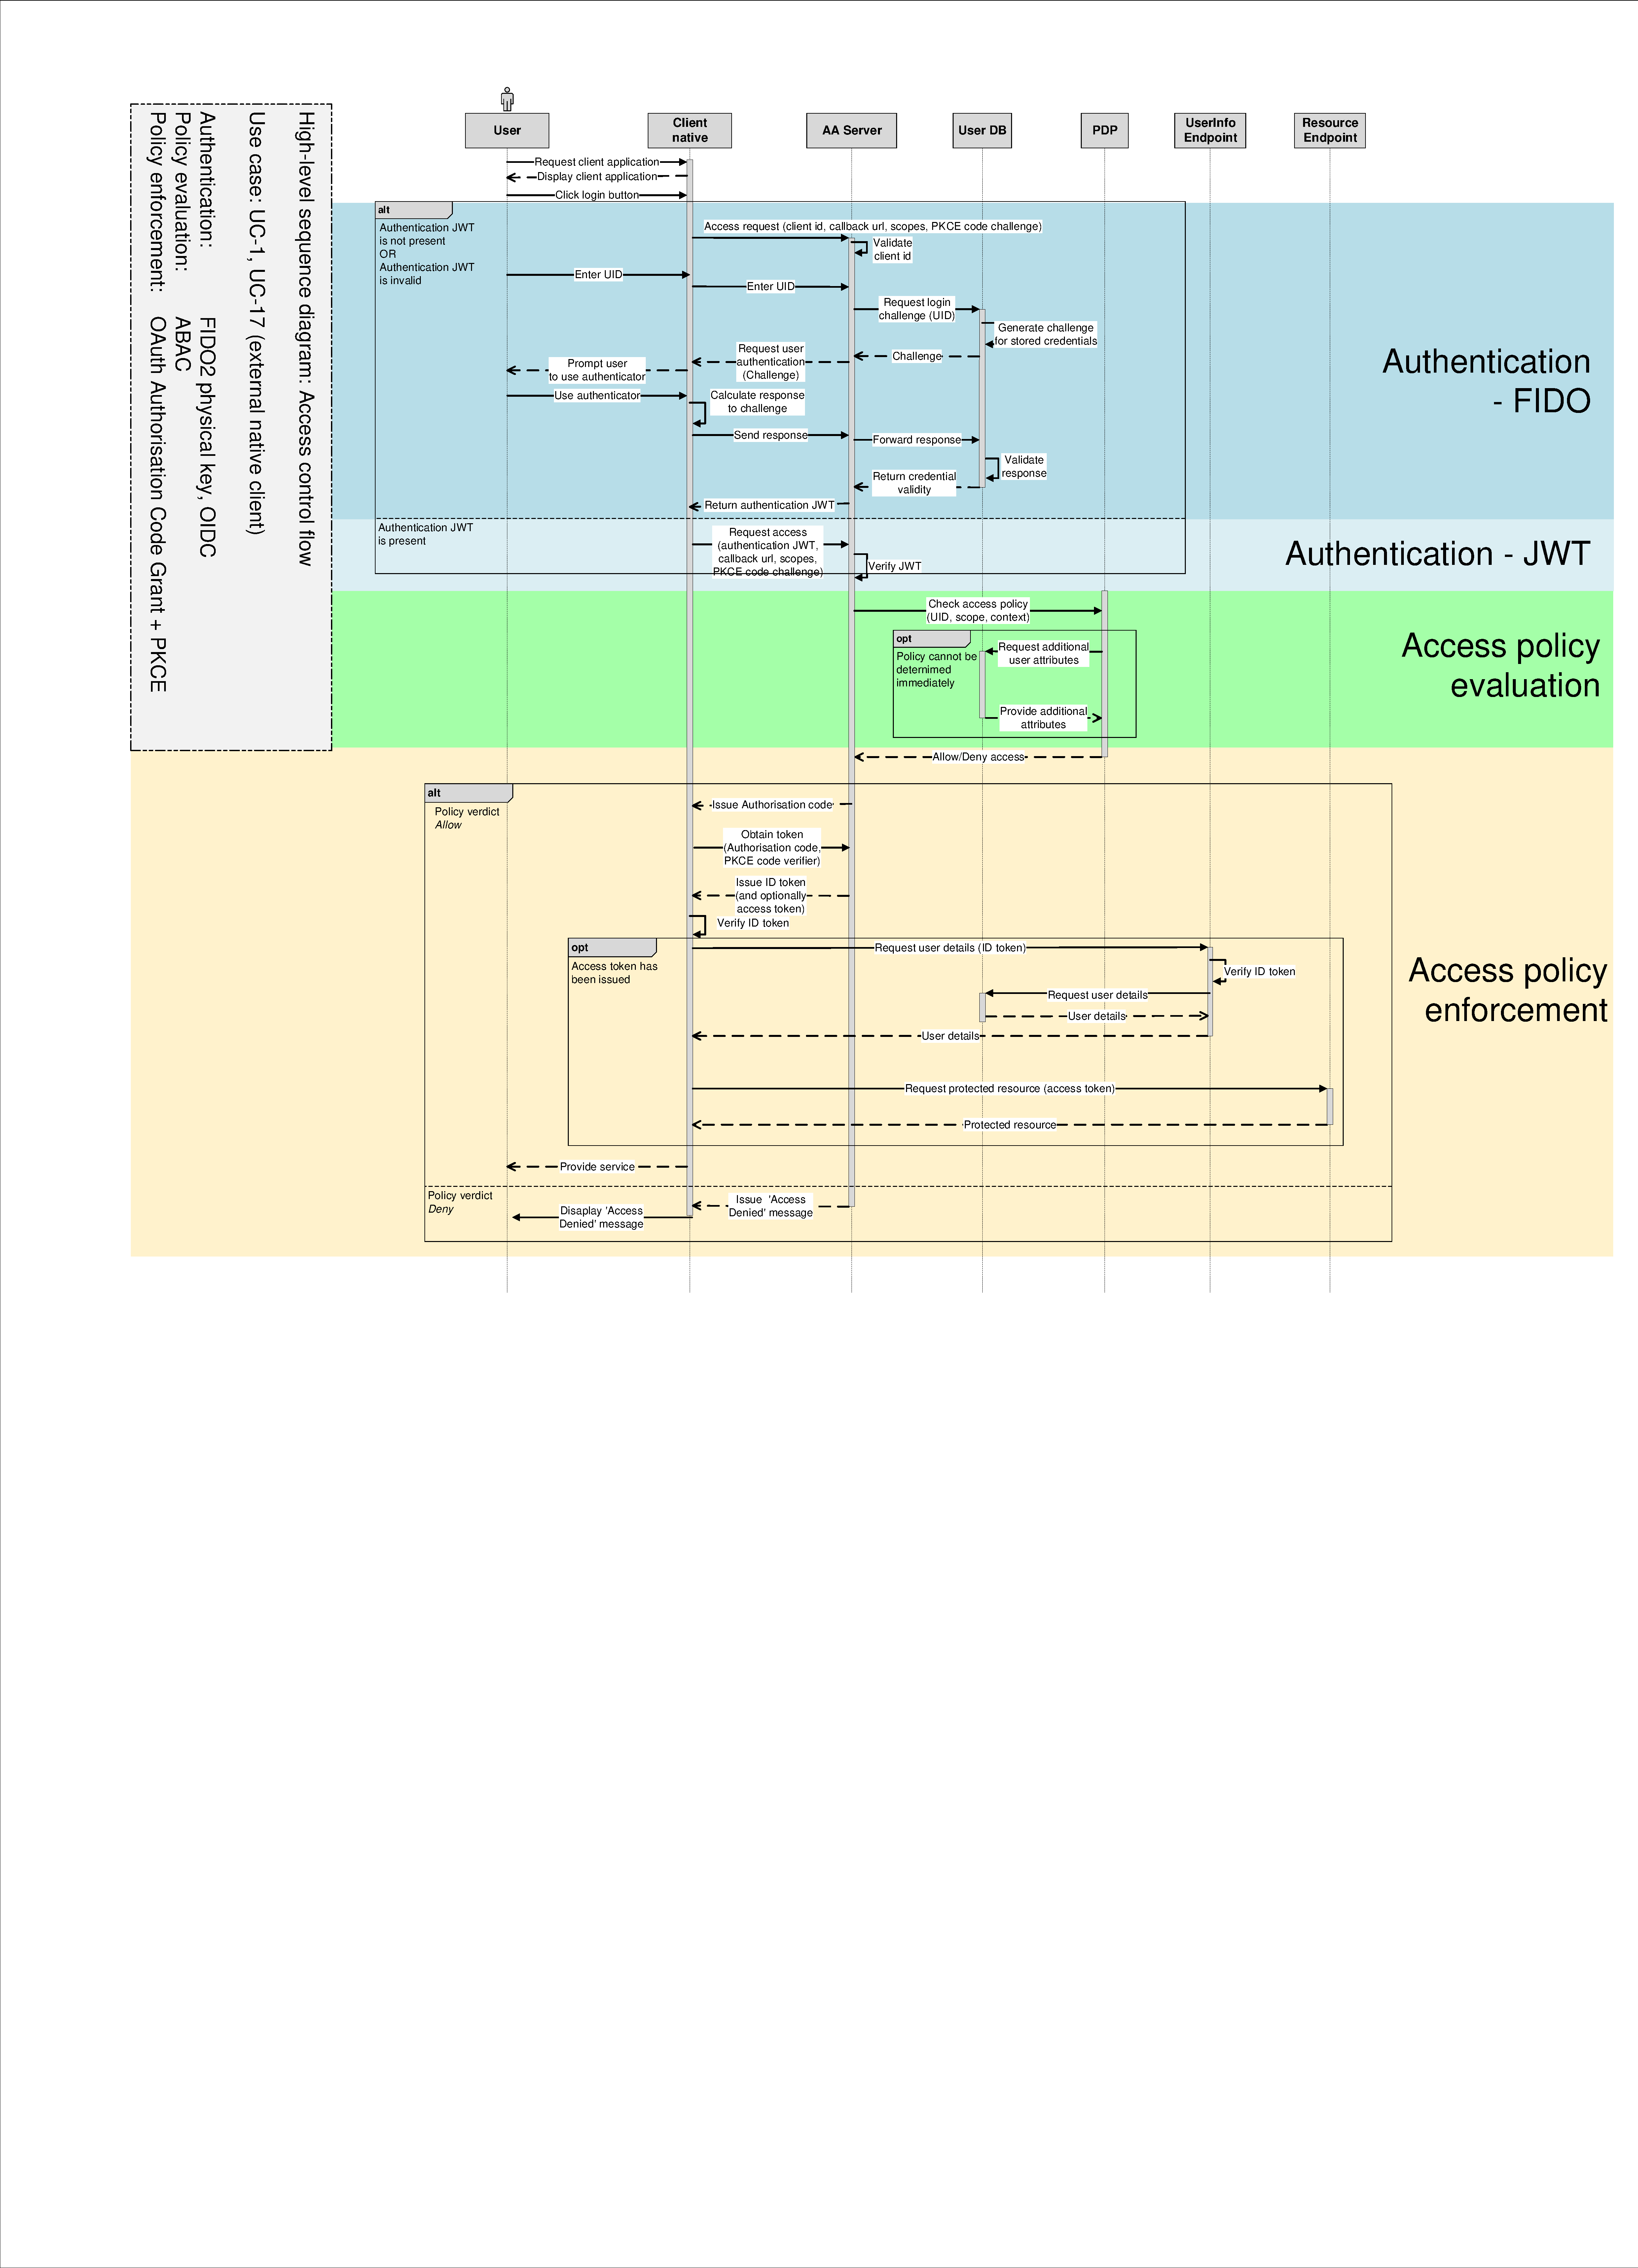
\includegraphics[width=1.2\textheight]{external-native}
\end{minipage}
% 
\subsection{Accessing an external online system with a web-server based client}
\begin{minipage}{\textwidth}
    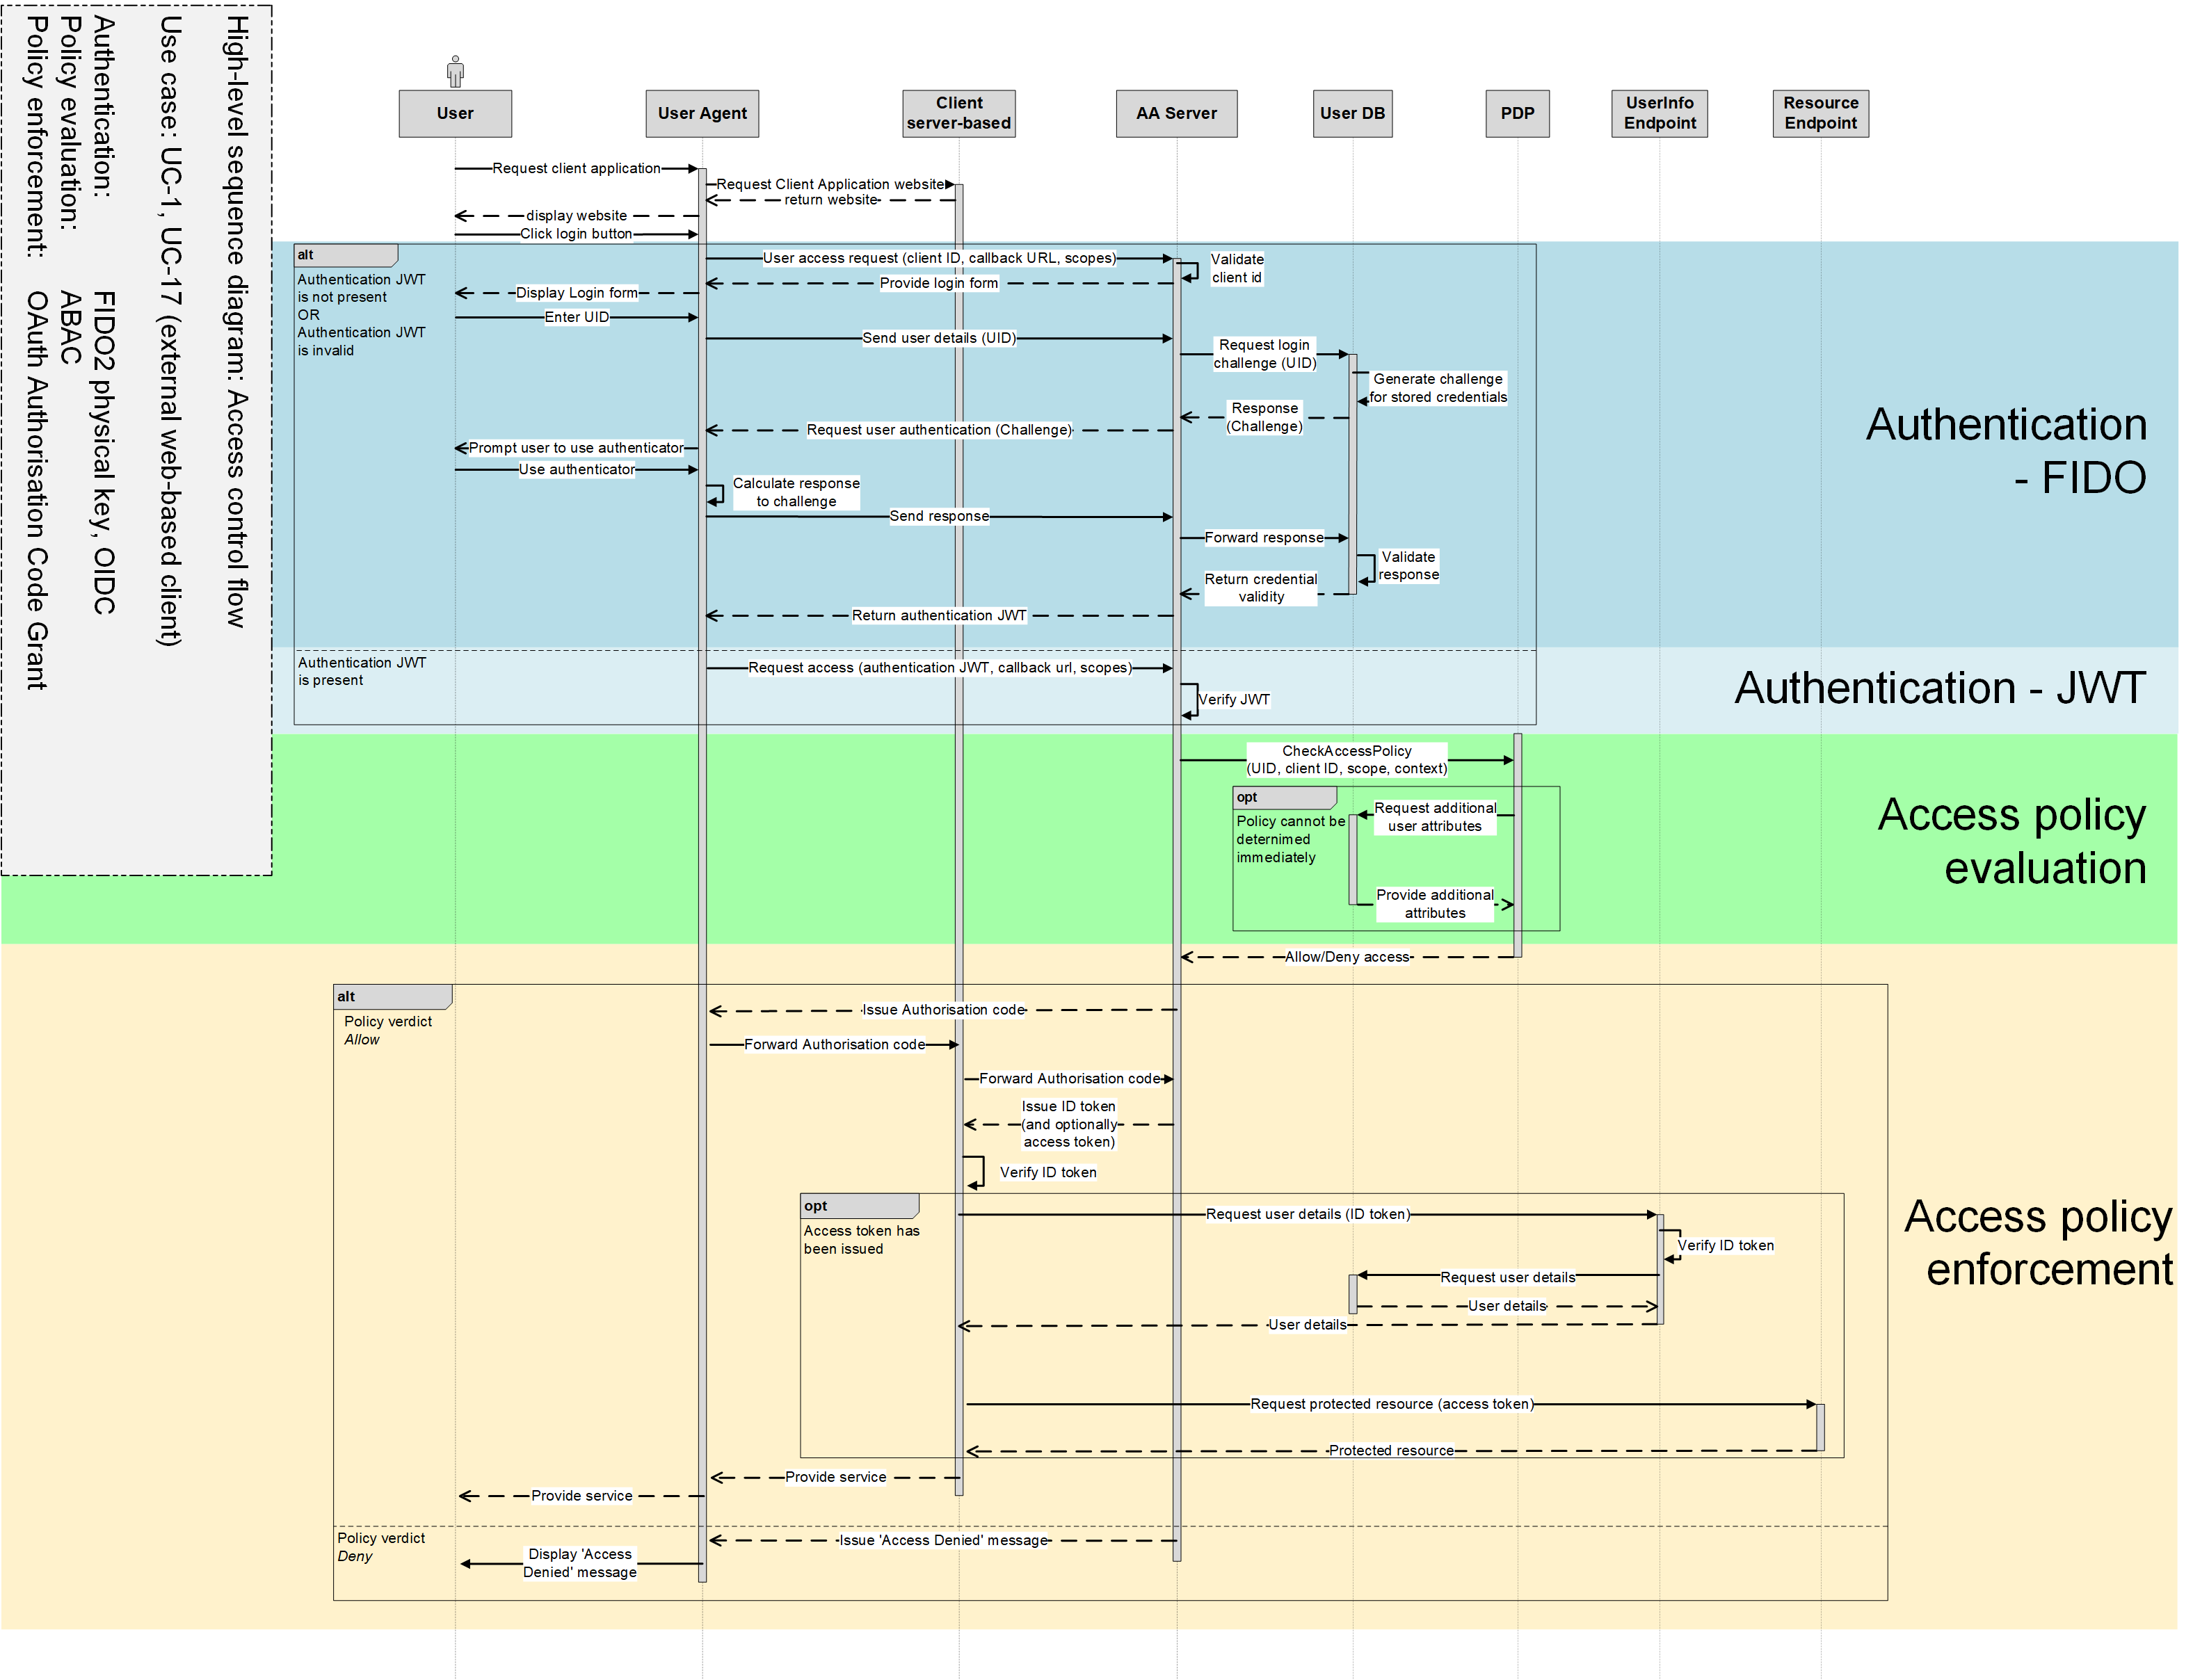
\includegraphics[width=1.25\textheight]{external-web}
\end{minipage}
% 
\subsection{Accessing an internal online system with a web-server based client}
\begin{minipage}{\textwidth}
    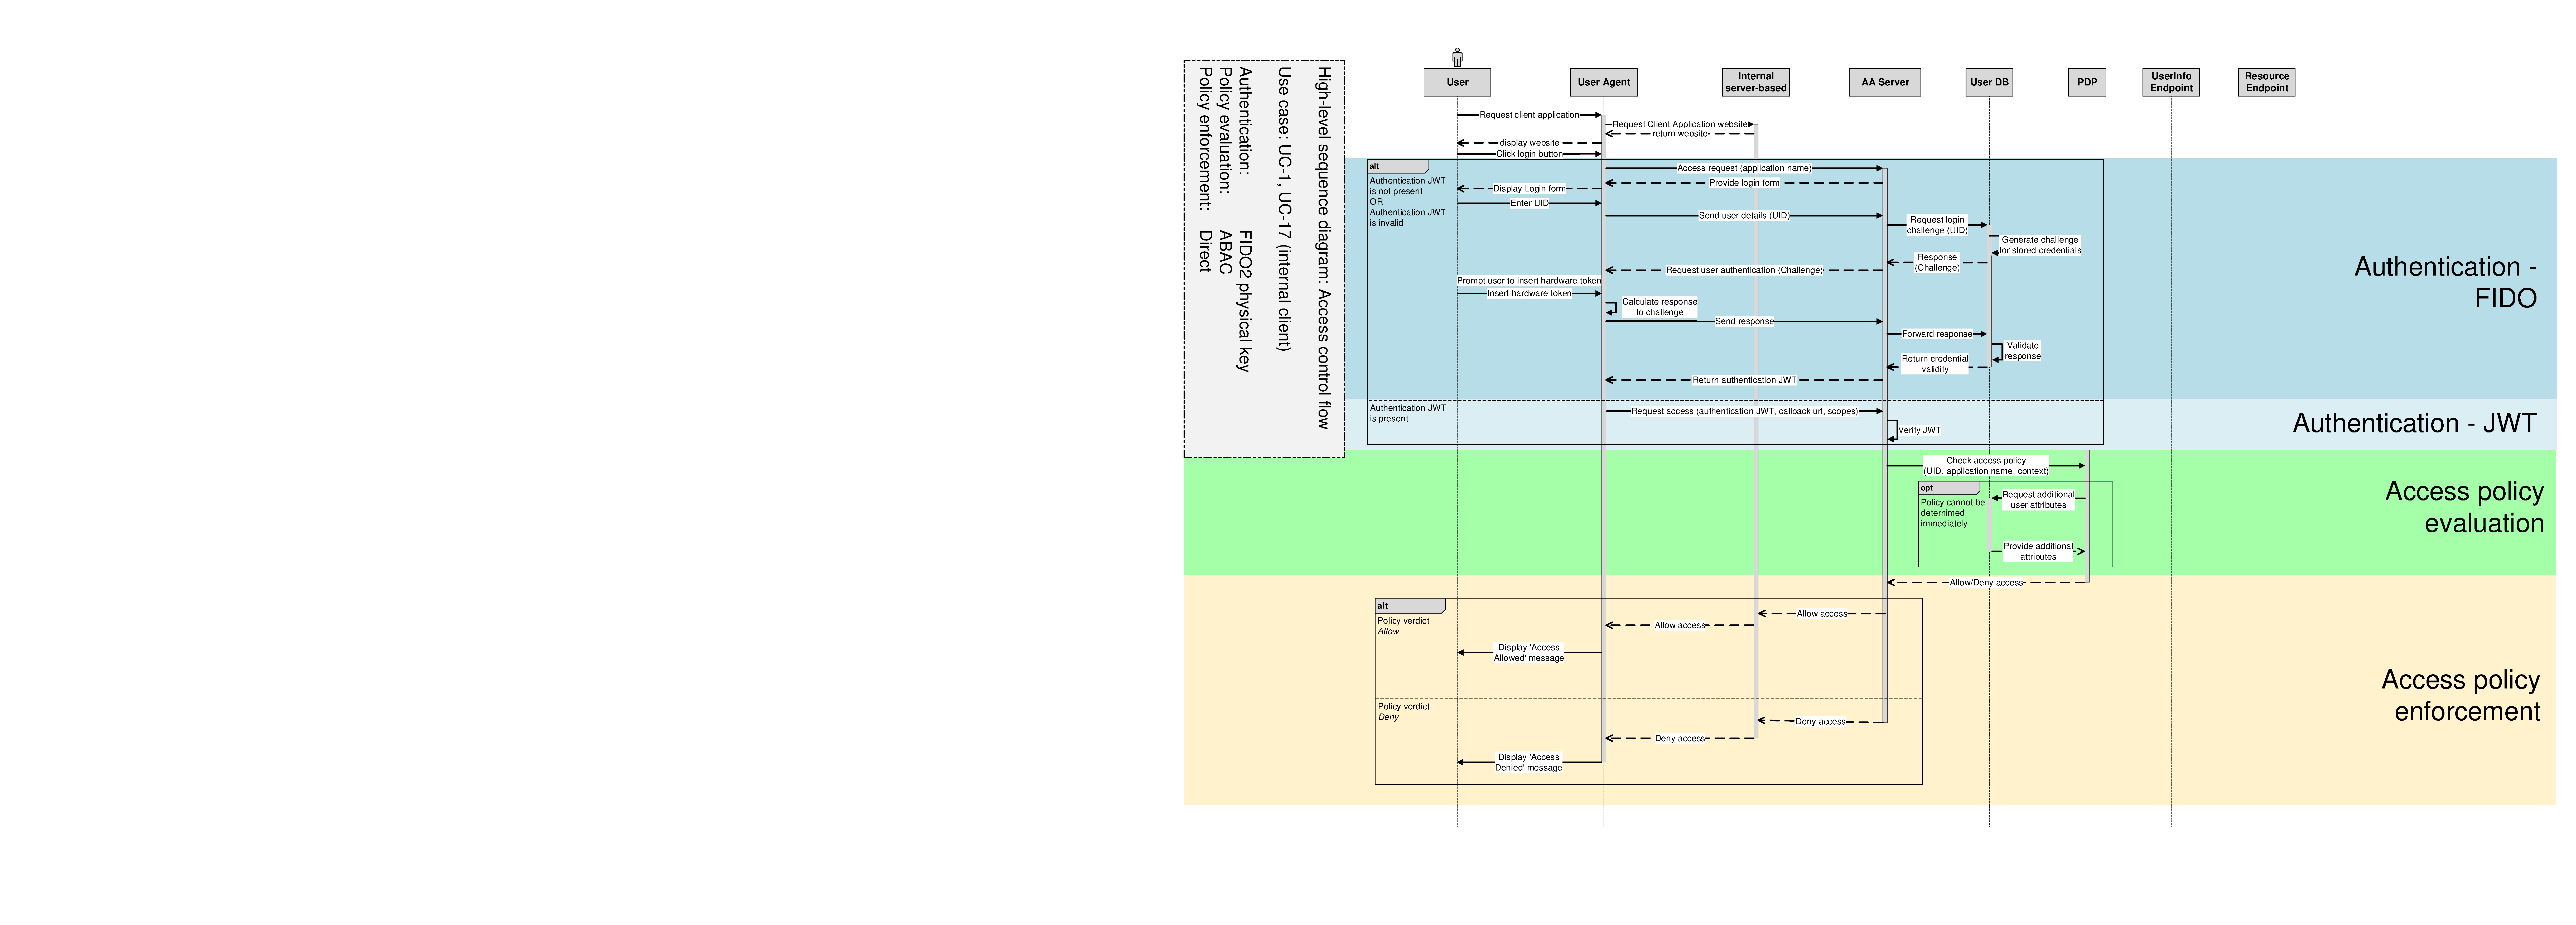
\includegraphics[width=1.35\textheight]{internal-web}
\end{minipage}
\end{landscape}
% \newgeometry{left=1cm,right=1cm,top=1cm,bottom=1cm,footskip=.4cm}
\restoregeometry

\end{document}